\documentclass{article}
\usepackage[spanish]{babel}
\usepackage[utf8]{inputenc}
\usepackage{graphicx}
\usepackage{color, colortbl}
\definecolor{LightOrange}{rgb}{1,0.90,0.74}
\newcommand{\tab}{\hspace*{2em}}

\begin{document}

\title{Pretotyping@Work\\[2ex] \large{Inventa Como Una Startup, Invierte Como Un Adulto}}
\author{Jeremy Clark\\Co-Fundador de PretotypeLabs\\[2ex] Traducci\'on - Oscar Rubio, Rodrigo Valdes\\[2ex] Primera Edici\'on}

% Definition of \maketitle
\makeatletter         
\def\@maketitle{
\begin{center}
{\Huge \bfseries \sffamily \@title }\\[4ex] 
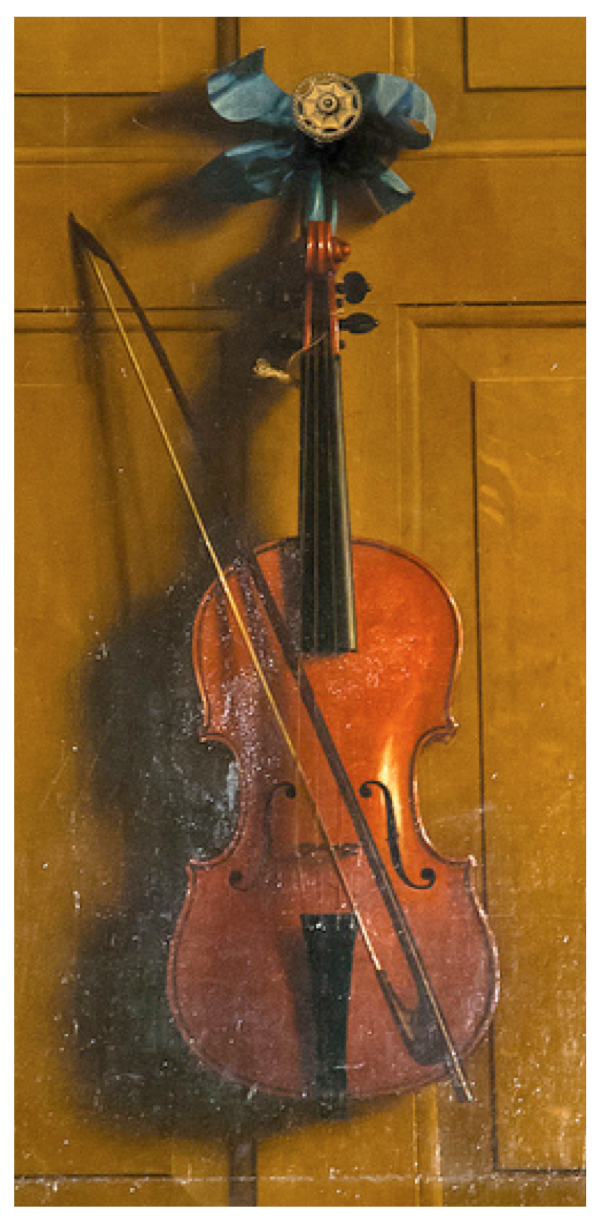
\includegraphics[width = 60mm]{cover.png}\\[4ex]
{\normalsize  \@author}\\[4ex] 
\end{center}}
\makeatother

\clearpage\maketitle
\thispagestyle{empty}
\newpage

\section*{NOTA DE AUTOR}

Este es un libro de econom\'ia. Antes de dejarlo caer como si estuviera en llamas y salir corriendo de la habitaci\'on, perm\'itanme explicar.	La econom\'ia es el estudio de la escasez de recursos y la elecci\'on; ayuda a clarificar los trade-off que enfrentamos cuando tomamos decisiones sobre d\'onde poner nuestro tiempo y dinero, cu\'ando y cu\'anto debemos gastar o ahorrar.     En el contexto de la innovaci\'on, la econom\'ia informa el tipo y n\'umero de innovaciones intentadas en un per\'iodo determinado - que tan atrevida, c\'omo se persigui\'o agresivamente, y c\'omo fue financiado.     Este libro describe un enfoque para la toma de decisiones de innovaci\'on que puede romper el enorme despilfarro de trade-offs hist\'oricos de los recursos.
\\ \\
El objetivo de este libro es permitir la aplicaci\'on pr\'actica de este enfoque - \textbf{\textit{pretotyping}} - dentro de las empresas establecidas que buscan mejorar la eficacia de sus procesos de innovaci\'on front-end.     Mi colega y amigo Alberto Savoia es el creador del t\'ermino preto-type y de gran parte del fundamento te\'orico para pretotyping.     Para una lectura entretenida y r\'apidamente digerible en el m\'etodo, recomiendo su excelente libro \textit{Pretotype It}.\footnote{``Pretotype It: Make sure you are building the right it before you build it right'', Alberto Savoia, 2011, disponible en amazon.com como una descarga kindle.}     Le debo a Alberto - y a muchos colaboradores en Google, donde abunda pretotyping - una deuda profunda, y de coraz\'on reconozco sus t\'ecnicas previas.
\\ \\
Este libro se basa en el taller \textit{Pretotyping@Work} que he desarrollado con Alberto, que hace de pretotyping un m\'etodo ense\~nable y repetible.     Como el libro est\'a destinado a ser le\'ido por los nuevos en pretotyping, habr\'a un poco de duplicaci\'on de conceptos para los iniciados, para los que se compensa con nuevas herramientas y perspectivas.
\\ \\
Por el feedback invaluable, refuerzo, y el desaf\'io constante, debo tambi\'en agradecer a mi esposa Petra y a Alberto por su paciencia en la revisi\'on de los escritos originales.     Gracias, finalmente, a los participantes de Alberto en mis discursos y talleres previos, incluyendo una versi\'on beta de el taller realizado en la Universidad de Stanford GSB en junio de 2012.
\\ \\
La foto de la portada es un \textit{trompe l'oeil} (enga\~na al ojo), la imagen de un viol\'in pintado sobre la puerta interior del State Music Room en Chatsworth House en Derbyshire, Inglaterra.     Fue pintado por Jan van der Vaardt en el siglo 18, y para m\'i, captura elegantemente la esencia de pretotyping: una impresi\'on fascinante de lo real que tiene \'exito por no ser lo que aparenta ser.
\\ \\
Dedico este libro a mi difunto padre, Peter Clark, ingeniero en mec\'anica, piloto, fabricante de soluciones.     \'El no era, en el sentido que hoy en d\'ia, un hombre centrado en el cliente, pero en el Reino Unido habr\'ian puesto sus esperanzas de medalla de oro si el reparar cosas fuese un evento Ol\'impico.


\newpage

\tableofcontents
\clearpage

\section{EL OBJETIVO DE ESTE LIBRO}

En la d\'ecada de 1980, IBM estaba en conversaciones con varios clientes importantes respecto una idea radical de productos: hardware y software que podr\'ian convertir palabras habladas en un texto en una pantalla. La tecnolog\'ia a\'un estaba a a\~nos de distancia, sin embargo los clientes parec\'ian muy entusiastas: muchos declararon que pagar\'ian generosamente para una soluci\'on de este tipo.
\\ \\
Tradicionalmente, IBM habr\'ia puesto en marcha un trabajo de I + D para desarrollar los algor\'itmos y los componentes electr\'onicos necesarios para presentar un prototipo. En el caso de la idea de Voz-a-Texto, sin embargo, un miembro del equipo sugiri\'o una alternativa intrigante: se debe \textit{pretender} tener la soluci\'on, para ver c\'omo los clientes realmente reaccionan a la nueva caracter\'istica.
\\ \\
Lo que el equipo hizo fue crear un set como laboratorio de pruebas con la forma de un espacio de oficina t\'ipico. Clientes ser\'ian informados sobre la soluci\'on de voz-a-texto y luego sentados en la ``oficina''. El cliente hablar\'ia a un micr\'ofono, dictando una serie de correos t\'ipicos, y ver\'ia casi inmediatamente como sus palabras aparecen en la pantalla en el escritorio en frente de ellos. Lo que los clientes no saben es que la salida electr\'onica estaba siendo producida por una mecan\'ografa en una habitaci\'on cercana, escuchando el dictado a trav\'es de auriculares.
\\ \\
Lo que el equipo de IBM aprendi\'o fue que, en la pr\'actica, a los clientes no les gustaba la soluci\'on, no a causa de defectos en el producto (el texto transcrito), si no que debido a una serie de desaf\'ios ambientales hasta ahora no vistos: hablar exig\'ia la garganta del sujeto, hab\'ia preocupaci\'on por la privacidad de material confidencial que el hablante no deseaba ventilar, y as\'i sucesivamente. La exposici\'on real a la soluci\'on propuesta invirti\'o por completo el entusiasmo de los clientes.
\\ \\
Lo que el equipo de IBM hab\'ia hecho era un \textit{pretend-otype}-: fing\'ir antes de hacerlo. Era m\'as que una prueba de concepto o una idea en un pedazo de papel (lo cual es completamente hipot\'etico). Era menos que un prototipo, que t\'ipicamente es un desarrollo primitivo pero funcional a una problem\'atica presentada. Era algo en el medio, un nuevo protocolo experimental que condujo a la pregunta fundamental en el coraz\'on de cada innovaci\'on.\\
Los clientes lo quieren?
\\ \\
Este libro convierte lo que el equipo de IBM hizo en un m\'etodo completo llamado Pretotyping, mientras que el ``pretender'' est\'a involucrado, este m\'etodo debe m\'as a la ciencia del complejo comportamiento de las artes esc\'enicas. El m\'etodo considera conceptos de la teor\'ia empresarial, aunque pretotyping es mas relevante para las empresas establecidas en los procesos de innovaci\'on que buscan aumentar su tasa de \'exito.
\\ \\
El libro desarrolla la teor\'ia y el m\'etodo de pretotyping con variados ejemplos y gr\'aficos, ademas proporciona herramientas pr\'acticas para que los lectores lo apliquen inmediatamente a innovaciones de todo tipo: producto, servicios y cambios internos.
\\ \\
Tenga en cuenta que este libro NO es un manual que cubra todos los procesos de innovaci\'on. Este libro propone una reflexi\'on profunda en el per\'iodo cr\'itico entre la conceci\'on de la idea y el desarrollo de productos, un tratado sobre c\'omo llegar m\'as lejos de forma mas r\'apida y con la menor cantidad posible de recurso desperdiciado e incertidumbre.
\\ \\
UNAS PALABRAS RESPECTO AL ``THE RIGHT IT''
\\ \\
Los lectores de \textit{Pretotype It} recordar\'an la definici\'on de Alberto del correcto ``\textbf{it}''. A lo largo de este libro, cualquier referencia a ``\textbf{it}'' se refiere a una nueva idea para un producto, servicio o iniciativa que pueda ser finalmente vendida al cliente final, utilizado interiormente de una empresa como una iniciativa de cambio, o usado entre dos empresas en un contexto de negocio a negocio (B2B). 
Esta lista de sin\'onimos podr\'ia ayudar:
\\ \\
Un ``\textbf{it}'' podr\'ia ser...
\\ \\
...Una \textbf{i}dea a in\textbf{t}entar
\\ \\
...Una \textbf{i}nnovaci\'on \textbf{t}ecnol\'ogica
\\ \\
...Una transformac\textbf{i}\'on in\textbf{t}erna
\\ \\
...Una herram\textbf{i}en\textbf{t}a para la innovaci\'on
\\ \\
Mantenemos la intenci\'on de destacar la amplia relevancia de los principios de pretotyping a muchos tipos de innovaci\'on radical, ya sea para llegar a un mercado de consumo o no. M\'as sobre esto en el cap\'itulo 6.

\clearpage
\section{COMPORTAMIENTO RACIONAL DE INVE(NT/RS)ORES}

Cuando las corporaciones innovan, los actores econ\'omicos claves son los \textbf{\textit{Inventores}}\footnote{Utilizar\'e el t\'ermino Inventor e Innovador de la misma manera para aprovechar la palabra Inve(nt/rs)ores. Algunos te\'oricos sostienen que hay diferencias importantes entre los dos roles, pero para los prop\'ositos de describir c\'omo la innovaci\'on atrae la inversi\'on, estas distinciones son irrelevantes El t\'ermino Inventor tambi\'en incluye equipos de inventores.} y los \textbf{\textit{Inversores}} o Inversionistas. Piense en ellos como los vendedores y compradores en un mercado de ideas. Esto es cr\'itico dado que tal como en la econom\'ia como un todo, los mercados de innovaci\'on corporativa en raras ocasiones funcionan de manera eficiente; de hecho, la mayor\'ia de las corporaciones favorecen de manera sistem\'atica las oportunidades mas incrementalmente seguras y poseen un prejuicio en contra de las ideas riesgosas y rupturistas. Para entender el porqu\'e de esto debemos observar el juego desde m\'as cerca , sus jugadores y la manera en que juegan.
\\ \\
Muchos empleados corporativos juegan un rol como \textbf{\textit{Inventores}}, tanto como parte fundamental su trabajo, as\'i como en una peque\~na proporci\'on. Los m\'etodos de los inventores var\'ian ampliamente de organizaci\'on a organizaci\'on, sin embargo actividades comunes son por ejemplo: explorar las necesidades de los clientes, de los nuevos mercados generando nuevos conceptos de servicios y productos, inventar nuevos enfoques de procesos y modelos de negocio, guiando estos inventos durante su desarrollo hasta un exitoso lanzamiento.
\\ \\
Es un poco clich\'e, sin embargo los inventores se revelan a partir de sus rasgos de \textbf{\textit{emprendimiento}}: En sinton\'ia con las posibilidades del futuro, optimistas, tendencia a la acci\'on, sin temor a los riesgos, y frecuentemente dotados de un sano desprecio por el status quo.
\\ \\
Los inversionistas o inversores son menos en n\'umero pero en general poseen una mayor autoridad. Los inversionistas son normalmente mandos medios a ejecutivos seniors que destinan recursos de la organizaci\'on para incentivar iniciativas de innovaci\'on. Los inversionistas tambi\'en son f\'aciles de identificar como los ``\textbf{\textit{adultos}}'' de las organizaciones: en sinton\'ia con el negocio, cautelosos, anal\'iticos y una tendencia hacia a conservar el status quo.
\\ \\
No es una sorpresa entonces, que los inventores a menudo ven a los inversores como lun\'aticos que minan las posibilidades de implementar sus imaginativas pero no probadas tesis respecto a los mercados y oportunidades en donde la compa\~n\'ia posee poca o ninguna experiencia significativa. Por otro lado los inversionistas a menudo visualizan a los inventores como trogloditas que viven en la oscuridad y asombrosamente imp\'avidos ante el buffet de posibilidades que se podr\'ian presentar.
\\ \\
Eso es a nivel de trato personal. Debemos considerar el contexto en los cuales estos personajes se desenvuelven y los scripts que tienen sus fundamentos. 
\\ \\
Inventores e inversionistas basan sus conversaciones dentro de un framework t\'ipico de procesos y est\'andares.

\begin{itemize}
  \item \underline{El Proceso anual de presupuesto} define los fondos disponibles para invertir en el desarrollo de proyectos de todo tipo. La mayor\'ia  de esos procesos son denominados como ``inelasticos'' - no existe mucho espacio de maniobra si las circunstancias cambian - lo que genera un l\'imite en relaci\'on a la cantidad proyectos innovadores y sus financiamientos en un a\~no determinado.
  
  \item \underline{El Business Case} es un documento que encapsula las afirmaciones de los inventores - algunas de ellas son suposiciones , otras son datos  - acerca de las necesidades del mercado, las caracter\'isticas de la soluci\'on, la oportunidad econ\'omica. Las compa\~n\'ias que usan ``Bussiness Case'' t\'ipicamente fijan una tasa de retorno m\'inima que se espera que las innovaciones generen antes de asegurar la inversi\'on.
  
  \item \underline{El New Product Development Proccess (NPD)} (De los cuales el m\'etodo propietario m\'as utilizado corresponde a Stage-Gate\footnote{Stage-Gate es marca registrada de Product Development Institute Inc.}) corresponde a un proceso estructurado para la administraci\'on de la innovaci\'on. El proceso especif\'ica actividades de desarrollo y niveles de definici\'on requeridos para pasar cada ``gate'' o revisi\'on de inversi\'on. La mayor\'ia de los procesos NPD requiere que los inventores cumplan con una serie de ejercicios para establecer una una estrecha conexi\'on entre la oportunidad, la  estrategia de la compa\~n\'ia y de sus competencias que se desarrollan a partir de la superaci\'on de cada obst\'aculo (gate).
\end{itemize}

Todos estos m\'etodos tienen buenas intenciones, pero existen fundamentalmente para el manejo de riesgo para las compa\~n\'ias circunscribiendo la decisi\'on al punto en que los proyectos sean considerados aptos para invertir. Las herramientas y reglas de este modelo - la selecci\'on inicial de proyectos, la tasa m\'inima de retorno de business case y el presupuesto inel\'astico - combinados generan al menos tres peligrosos efectos al proceso de Innovaci\'on rupturista.

\begin{enumerate}
  \item Los inventores de convierten en ``\textbf{EMO}'', o \textbf{\textit{exageran, manipulan y ocultan}} con el objetivo de complacer a los inversionistas. Los riesgos y los imprevistos son desestimados y las proyecciones de ganancias toman la forma de un bast\'on de hockey, es decir, existe un peque\~na curva de costos al comienzo que parecen triviales los cuales se compensan con un siempre creciente flujo de ganancias a partir del lanzamiento.
  
  \item Los inversionistas se tornan \textbf{exc\'epticos} ante cualquier petici\'on de financiamiento para proyectos de innovaci\'on rupturista, bajando las expectativas respecto a las ganancias y multiplicando los posibles efectos en costos y tiempos presupuestados. Despu\'es de todo, los inversionistas han presenciado este tipo de shows anteriormente.
  
  \item Un perjudicial \textbf{sesgo} por invertir en oportunidades que se asemejen a los productos, servicios y mercados actuales.
\end{enumerate}

Me gustar\'ia ver la primera etapa de este dialogo entre inventores e inversionistas cambiar dram\'aticamente. El patr\'on descrito anteriormente se caracteriza por un peque\~no n\'umero de revisiones infrecuentes y orientadas el detalle, en donde las reputaciones est\'aban en juego y los hechos son muy pocos. Cualquiera sea la ``tasa limite de inversi\'on'', cada proyecci\'on inevitablemente ser\'a alcanzada, pero tomara meses y mucha inversi\'on antes de que los clientes reales den su veredicto en el mercado.
\\ \\
    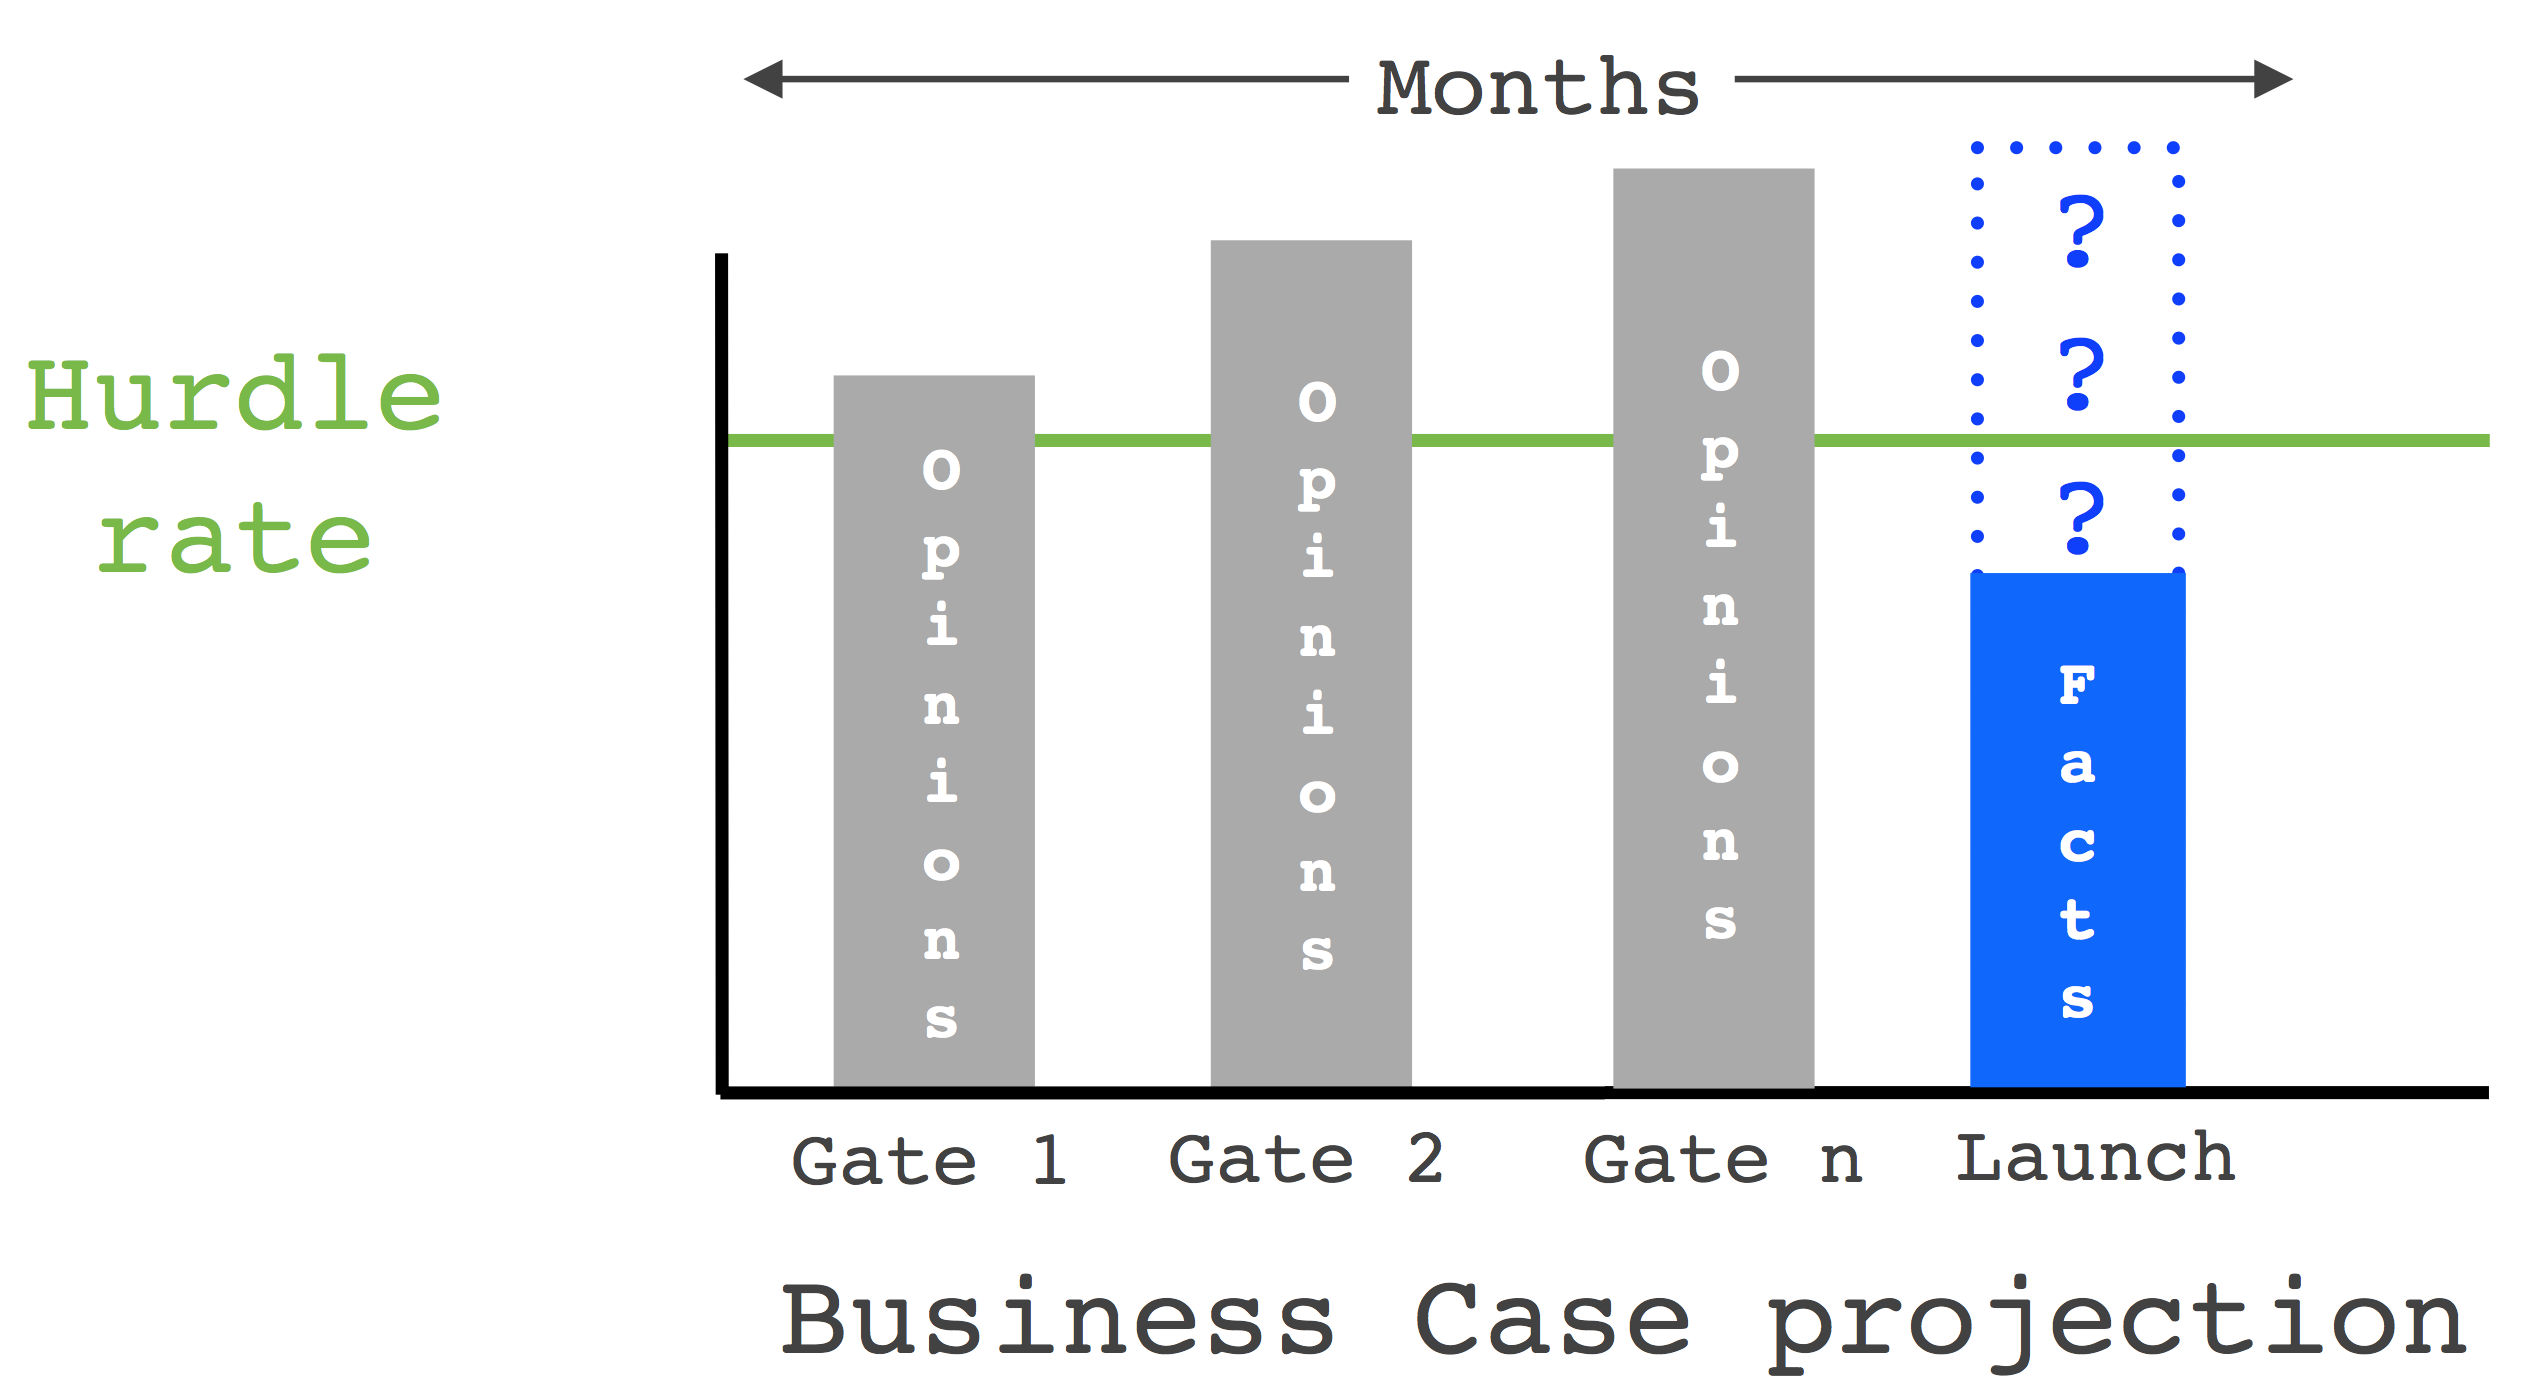
\includegraphics[width=1.0\textwidth]{bussines_case_projection}
\\ \\

Ambos lados merecen mejores herramientas. El marco apropiado para ese di\'alogo es mediante muchas conversaciones peque\~nas, ocurriendo frecuentemente y marcadas por peque\~nos experimentos que proporcionen datos reales respecto a si el \textbf{\textit{``it''}} apropiado se est\'a financiando. El inventor y el inversionista deber\'ian negociar umbrales de inter\'es de mercado que estimular\'a la continuaci\'on de los experimentos, para posteriormente mapear los primeros test para elevar el nivel de confianza a partir de peque\~nos incrementos.
\\ \\ \\
    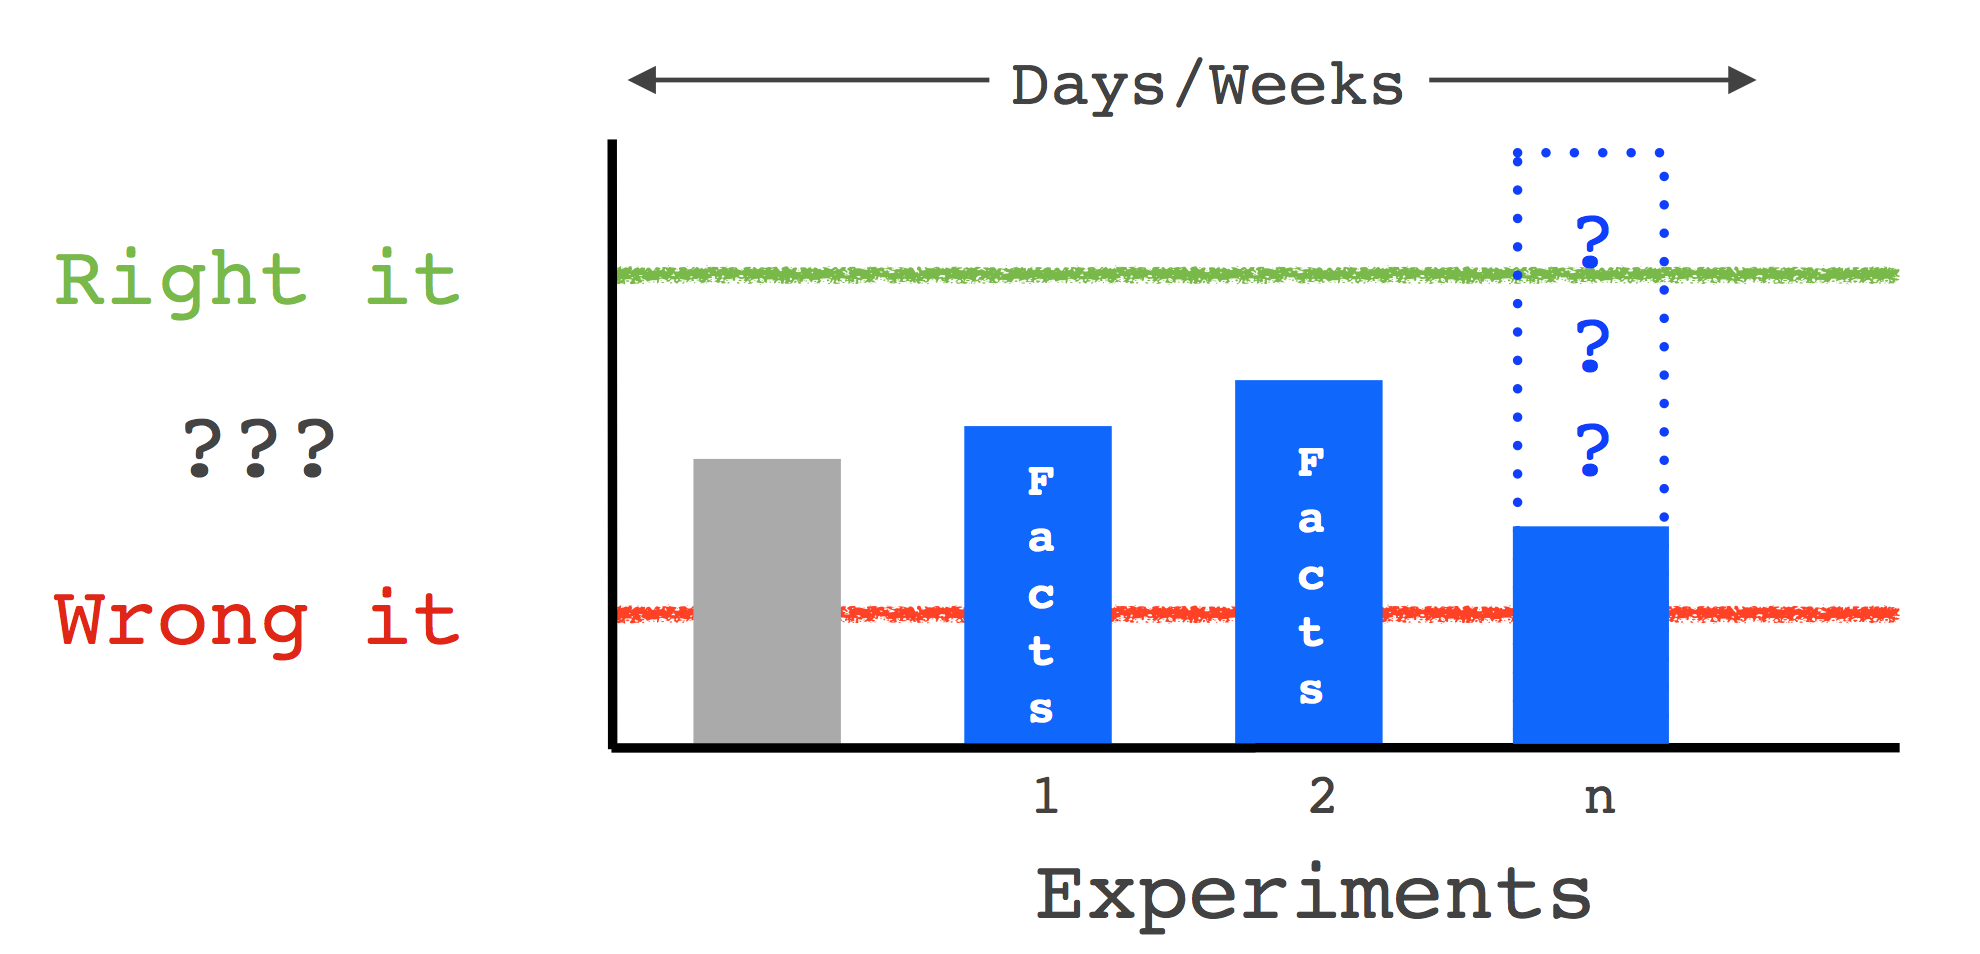
\includegraphics[width=1.0\textwidth]{experiments}
\\ \\
Esta negociaci\'on entre inventores e inversores sobre el nivel de inter\'es del mercado, generar\'a un apoyo continuo, lo cual es la innovaci\'on fundamental aqu\'i. Esto deber\'ia ocurrir para cada oportunidad. Tenga en cuenta que este di\'alogo no cambia las probabilidades de \'exito en absoluto: s\'olo produce un hecho-resultado anticipado, lo que permite m\'as oportunidades para ser exploradas y m\'as agilidad en la cartera de innovaci\'on. M\'as sobre esto m\'as tarde.
\\ \\
En lugar de decir NO por defecto, los inversores deben decir reflexivamente S\'I a la investigaci\'on inicial, a la vez se espera que los inventores se manifiesten r\'apidamente con DATOS. Los inventores deber\'ian aprender a entregar valor r\'apidamente priorizando la demanda como la variable clave, buscando el equilibrio de todas las ideas en fase inicial en un estado \textit{revealed-preference testing}\footnote{Revealed-preference testing es un concepto crucial para los pretotypers. Los economistas usan el t\'ermino para describir una prueba en la que el comportamiento de un sujeto puede ser tomado como id\'enticos a sus creencias. Una mejor definici\'on para nuestros prop\'ositos es: dise\~nar un experimento en el que usted puede pedir un \textit{compromiso} m\'as que una \textit{opini\'on}. Pruebas revealed-preference proponen ``Lo har\'as ...?'' No ``Quieres que ...?''.} y nunca obsesionarse de un concepto no probado.
\\ \\
Este es un hermoso sue\~no y tengo un m\'etodo para proponer. No va a ser f\'acil, ya que el proceso predeterminado est\'a profundamente arraigado en nuestra instituciones. Para entender lo que esperamos ganar al cambiar el dialogo Inventor-Investor, primero tenemos que enfrentar las razones detr\'as el fracaso de la mayor\'ia de las ideas en etapa temprana.

\clearpage
\section{INVENTA COMO UNA STARTUP}

Inventores, les ha pasado esto? Un alto ejecutivo inversor anuncia que su compa\~n\'ia est\'a buscando la SIGUIENTE IDEA DEL BILLON DE DOLARES: ustedes son los elegidos para encontrarla desafiando LAS VIEJAS PRACTICAS, BUSCANDO NUEVAS NECESIDADES DE LOS CLIENTES, y sobre todo, pensar fuera de la CAJA!
\\ \\
Pasan algunas semanas y tu produces los frutos de tu trabajo.
\\ \\
Qu\'e sucede? Shock!: los inversores seleccionan y financian las ideas mas seguras, en su mayor\'ia ideas incrementales! El cinismo y el consumo de anti\'acidos se disp\'ara por las nubes.
\\ \\
Por qu\'e ocurre esto? Porque la clase inversionista ejecuta el negocio actual de la empresa, y los fondos que la empresa invierte en nuevas ideas son enormes. Mientras mas novedosa sea la idea, menos pareciera que esta generar\'a los flujos de ingresos que el negocio necesita hoy. Ellos no quieren perder los fondos que podr\'ian utilizarse en extensiones de l\'inea. Lamentablemente, el historial de avances rompedores intentados por la empresa apoyan esta visi\'on de las cosas.
\\ \\
Como llegar a los inversores que piensan diferente? Ens\'e\~nales a entender por qu\'e tu nueva idea probablemente fallar\'a, y por qu\'e una prueba r\'apida y barata permitir\'a que todo se discuta en base a los datos y no las opiniones.

\subsection{Las Leyes del Fracaso}

El primer problema a enfrentar cuando se trabaja con inventores es el idealismo. Inventores viven en un mundo en el que todo es posible, donde nada se ha desmentido ni ha decepcionado, donde los avances - y las riquezas que seguramente vendr\'an - son el horizonte pr\'oximo.
\\ \\
Despierta Pollyanna\footnote{Pollyanna es una novela de Eleanor H. Porter publicada en el a\~no 1913, Pollyanna se usa para describir a una persona que es optimista de manera exagerada.}: LA MAYORIA DE LAS IDEAS NUEVAS FALLAN.
\\ \\
Esto es lo que Alberto y yo llamamos la Primera Ley del Fracaso, y lo que carece en profundidad lo compensa en veracidad. Nadie quiere admitirlo, especialmente aquellos cuya vida depende de cuidar presupuestos para instalaciones de I + D, centros de innovaci\'on y sitios de brainstorming; pero la evidencia es abrumadora.
\\ \\
Un reciente estudio de Nielsen sigui\'o el \'exito en el mercado de 24.543 nuevos productos durante el primer a\~no despu\'es de su lanzamiento. Sus conclusiones se enmarcan en t\'erminos de \'exito en relaci\'on con las expectativas previas al lanzamiento:
\begin{table}[h]
\centering
    \begin{tabular}{|l|l|}
    \hline
    Fracaso       & 27\% \\ \hline
    Decepci\'on & 16\% \\ \hline
    Cancelado    & 37\% \\ \hline
    Exito      & 14\% \\ \hline
    Estrellato         & 6\%  \\ \hline
    \textbf{Total}        & \textbf{100\%} \\ \hline
    \end{tabular}
\end{table}
\\
Las distinciones entre las categor\'ias son irrelevantes para nuestro prop\'osito, pero como un ejercicio de reflexi\'on,  si se suman ``Fracaso'', ``Decepci\'on'' y ``Cancelado'' se obtiene un 80\%. Eso deja un 20\% de probabilidad de alcanzar el ``Exito'' o el estado de ``Estrellato'', los que para nuestros prop\'ositos cuentan como una victoria.
\\ \\
Hay un corolario esencial para la Primera Ley del Fracaso:
\\ \\
\textbf{La mayoria de las ideas fallan, \underline{incluso si estan bien ejecutadas}}\footnote{``New Product Development: product launches hindered by major challenges'' Revista Consumer Goods Technology, Agosto del 2011}
\\ \\
En una encuesta realizada el 2011 a empresas de bienes de consumo, el 70\% de los encuestados report\'o que la Baja calidad del producto ``casi nunca'' es una causa de fracaso para un producto nuevo, mientras que el 67\% de manera similar culp\'o ``problemas t\'ecnicos o regulatorios''. Por otro lado, el 45\% de los encuestados citaron ``La falta de datos relativos al futuro valor econ\'omico del producto'' como causa ``frecuente o casi siempre'' de fracaso, y el 41\% seleccion\'o ``la falta de datos para validar que el producto se dirige a una necesidad real del mercado''.
\\ \\
Esto significa que las tasas de fracaso en el estudio Nielsen no son el resultado de una mala ejecuci\'on de una buena idea, si no que indican una robusta ejecuci\'on y puesta en marcha de una premisa mal concebida. O, como preferimos decirlo, \textbf{la mayor\'ia de los fallos tienen como origen una buena ejecuci\'on, pero un ``it'' equivocado.}
\\ \\
En t\'erminos pr\'acticos, esto significa que las probabilidades de cualquier idea de convertirse en \'exito son muy bajas (del orden del 20\%). Para las peque\~nas empresas en b\'usqueda de nuevas ideas de productos, lo m\'as probable es que se quedaran sin presupuesto y tiempo antes de lograr el \'exito. Para startups financiados, inversores (generalmente empresas de capital de riesgo) enfrentan estas probabilidades manteniendo un estricto control sobre el flujo de caja y presionando a los Inventores (fundadores de la empresa) a ``pivotear'' a un nuevo producto y / o estrategia de modelo de negocio, tan pronto como el actual pareciera que va a fracasar. Compa\~n\'ias sin Inversores atentos e Inventores flexibles probablemente se quedaran sin dinero y tiempo tratando de poner a prueba su idea original.
\\ \\
Las empresas m\'as grandes y mejor establecidas pueden absorber mejor las p\'erdidas gracias a bolsillos m\'as grandes, pero eso s\'olo hace que la acumulaci\'on de despilfarro de recursos sea peor. Alberto llama a este efecto la Rueda del Fracaso: en promedio, cada vuelta de la rueda - o ``apuesta'' en una nueva idea de producto - produce una respuesta positiva en 1 de cada 5 veces en el mercado. Las otras 4 apuestas perder\'an todo, ya como todos saben, la casa siempre gana.
\\ \\
Las probabilidades en La Rueda del Fracaso son a\'un peores para innovaciones radicales, nuevas ideas que ofrecen una dram\'atica mejora precio-rendimiento, o que superan las expectativas de los usuarios, en relaci\'on con las ofertas actuales. Los estudios confirman que los consumidores est\'an cansados de que los avances significativos constituyen una proporci\'on muy peque\~na de todas las presentaciones de nuevos productos. Los encuestados en el estudio \textit{CGT/Sopheon study of company-reported product innovations} clasifican un 18\% de los nuevos lanzamientos de productos como ``muy innovador'', mientras que el 61\% son ``extensiones de l\'inea'' o ``cambios en productos o embalajes''.
\\ \\
El estudio de Nielsen dividi\'o 24.543 nuevos productos en un n\'umero de categor\'ias en funci\'on de su grado de innovaci\'on:
\begin{table}[h]
\centering
    \begin{tabular}{|l|l|l|}
    \hline
    \textbf{Categoria}                      & \textbf{\# de productos} & \textbf{\% de productos} \\ \hline
    Rupturistas                    & 334                 & 1.4\%                   \\ \hline
    Extensi\'on de linea o categor\'ia & 1705                & 6.9\%                   \\ \hline
    ``Me too''                       & 18814               & 76.7\%                  \\ \hline
    Otros (estacional, etc)        & 3690                & 15.0\%                  \\ \hline
    \textbf{Total}                          & \textbf{24543}               & \textbf{100\%}                   \\ \hline
    \end{tabular}
\end{table}
\\
Como se puede ver en la tabla, la mayor\'aa de los nuevos productos puestos en marcha fueron clasificados como ``Me too''. Por qu\'e es esto? Aqu\'i es donde ocurren los lanzamientos de bajo riesgo; ya sea por la misma empresa o la puesta en marcha de la competencia, ya se ha validado la presencia de un mercado y la voluntad de los los compradores a pagar por soluciones en estas categorias. No es de extra\~nar que casi 19.000 de esos 24.543 nuevos productos eran versiones ``mejor / m\'as r\'apido / m\'as barato'' que las soluciones existentes.
\\ \\
El problema con esta estrategia "following" se revela comparando la primera y segunda tabla. Si la mayor\'ia de los productos nuevos se justifican con referencia al rendimiento actual del mercado de ofertas, por qu\'e muchos terminan en fracaso, decepci\'on, o cancelado? La competencia, por supuesto!: cada nueva oferta se une a filas de ofertas comparables y, en la mayor\'ia de los casos se canibalizan las ventas que de otro modo habr\'ian ido a un producto de la competencia. La mayor\'ia de las extensiones y los productos de imitaci\'on no aumentan el tama\~no del pastel del mercado, solo se agrega un nuevo actor al n\'umero de rebanadas cortadas de ella.
\\ \\
La peque\~na fracci\'on de innovaciones rompedoras, por el contrario, representan la mejor oportunidad de una empresa para rentabilidad sobre el promedio. Los avances rompedores contribuyen de manera desproporcionada a los ingresos y las ganancias, y esta importancia esta aumentado\footnote{``Survival of the Fattes'' by Raynor, Ahmed \& Guszcza, Deloitte Review, muestra c\'omo las empresas m\'as din\'amicas, y creadoras de valor generan retornos cada vez m\'as asim\'etricos. Desde el 2001, la rentabilidad media de los activos (ROA) de las empresas con percentil 100 ha variado 4x-8x, esto incluso ocurre en empresas en los percentiles 90 - 99!}. Sin embargo, para las innovaciones rompedoras, las probabilidades de la Rueda del Fracaso son a\'un peores: los datos de medio a largo plazo sugieren que s\'olo el 5\% de los intentos, o 1 vuelta de 20, tienen \'exito.
\\ \\
A primera vista, aparentemente los Inventores enfrentan una compleja decisi\'on: alcanzar un 20\% de probabilidad de obtener rentabilidad mediocre mediante el desarrollo de productos ``Me too'' o perseguir el 5\% de probabilidad de rentabilidad anormal a trav\'es del desarrollo de innovaci\'on no probada en ning\'un mercado.
\\ \\
Los inventores podr\'ian escapar a la paradoja si pudieran descubrir que ideas, sobre todo los avances rompedores (especialmente en una etapa de desarrollo temprana) fueron los ganadores y descartar los otros. A falta de una bola de cristal o la m\'aquina del tiempo, c\'omo podr\'ian los Inventores llevar a cabo este truco? Mediante apuestas en la Rueda del Fracaso de una manera m\'as inteligente: gastando cantidades mucho m\'as peque\~nas de tiempo y dinero con la idea de validar el mercado y demanda. \textbf{No se puede cambiar las probabilidades, pero si se puede cambiar la forma de jugar.}
\\ \\
Para ver c\'omo esto funciona, hay que hacer un viaje a un lugar maravilloso llamado Thoughtland (La tierra de los pensamientos).
\\ \\
THOUGHTLAND
\\ \\
Thoughtland es el h\'abitat natural de la mayor\'ia de los inventores y el lugar de nacimiento de todas las ideas. Es un maravilloso lugar de posibilidades infinitas. Las ideas son abstracciones hechas solamente de material conceptual.
\\ \\
Como tales, las ideas se pueden compartir con los dem\'as pero no de una manera real. Las Ideas s\'olo pueden tener opiniones por medio de una respuesta que presenta dos problemas fundamentales:

\begin{enumerate}
  \item Falsos Positivos: Toda idea puede ser un \'exito!
  \\ \\
  Recuerden a Webvan, los creadores de la idea de abarrotes ordenaron en l\'inea y luego entregado a su puerta? Concebido durante el primer boom de internet a finales de los a\~nos 90, la idea detr\'as de Webvan era un \'exito instantaneo en Thoughtland. Todo el mundo le dio un pulgar hacia arriba, y por qu\'e no? Parec\'ia sencillo, c\'omodo, ten\'ia ese gusto a genialidad estilo por-que-no-se-me-ocurri\'o-antes.
\\ \\
Los Inventores de Webvan, dirigidos por Louis Borders, procedieron a recaudar m\'as de \$122 millones de d\'olares en capital de inversores incluyendo Goldman Sachs y Sequoia Capital. Una oferta p\'ublica ofrecida en 1999 agreg\'o un adicional de \$375M; en total, Webvan recaud\'o m\'as de \$1B en la b\'usqueda de su idea. Estos fondos se usaron para construir una sofisticada p\'agina web de comercio electr\'onico, as\'i como una red de centros de distribuci\'on refrigerados en 26 mercados importantes y ademas se compr\'o una flota de de camiones para las entregas. Lanzada con bombos y platillos, la demanda inicial de \'ordenes impulsada por la curiosidad disminuy\'o r\'apidamente, dejando a los inversores de Webvan totalmente decepcionados y con un fracaso tremendo. Webvan solicit\'o la quiebra en Julio del 2001.
\\ \\
Qu\'e sali\'o mal? Los datos de Thoughtland sobre Webvan era enga\~nosos: las personas a las que se hab\'ia formulado una pregunta hipot\'etica sobre una idea abstracta de servicio, preguntas\footnote{Esto es, por supuesto c\'omo funcionan los grupos de enfoque, gran parte de los recursos mal gastados de los inventores se pueden atribuir a los datos Falsos Positivos obtenidos en reuniones voluntarias con clientes existentes donde las preguntas hipot\'eticas est\'an hechas sin mucho riesgo.} como ``Quieres usarlo?'', resultaron ser mucho menos entusiastas cuando se encontraron con un servicio totalmente funcional y se volvi\'o a preguntar ``Va a utilizarlo?''.
\\ \\
Falsos Positivos son un fen\'omeno muy difundido: se producen en todos los sectores de la econom\'ia, son dirigidos por expertos reconocidos en los campos de inversi\'on, comercializaci\'on y desarrollo de productos. Estos son algunos Falsos Positivos famosos que resultaron ser espectaculares ``wrong \textbf{\textit{it}}'' en el mercado:

\begin{itemize}
  \item La pel\'icula de Disney ``John Carter'' (Costo: \$275M + \$100M en marketing)
  \item Sistema telef\'onico satelital Motorola Iridium (\$6B por 66 Satelites)
  \item Transportador Segway (~\$180M en financiamiento)
  \item Pontiac Aztek (\$200M+)
  \item Google Wave (~\$20M-\$30M)
  \item Nueva Coca-Cola o Pepsi (estimado \$50M cada una)
\end{itemize}

  \item Falsos Negativos: Toda idea puede ser un fracaso!
  \\ \\
Qui\'en puede ignorar Twitter? Cuando escuch\'o por primera vez del servicio, cu\'al fue su reacci\'on? Algunos pudieron haber pensado que era un intrigante experimento de micro-difusi\'on en tiempo real (aunque a\'un no es claro para m\'i, que evidencia hubo de que se trataba de un espacio sin explotar para las personas). Seguramente muy pocos intuyeron que ser\'ia una herramienta critica para impulsar la revoluci\'on democratica de la Primavera \'Arabe. El discurso de Twitter fue recibido con incredulidad y curiosidad, tal como cuando un perro inclina su cabeza tratando de entender algo.
\\ \\
A pesar de esto, sus inventores continuaron con la idea, desarrollaron la plataforma y lanzaron el servicio en Julio del 2006.    En primavera del 2012, los 500M de subscriptores en Twitter posteaban 340M de ``tweets'' por d\'ia y el rol del Twitter en el universo de noticias importantes y de ultimo minuto (como el choque del jet de US Airways en el rio Hudson en Enero del 2009), establecieron la relevancia del servicio.
Inevitablemente, tal cantidad de usuarios alrededor de la plataforma crearon oportunidades para generar utilidades, y seg\'un algunas estimaciones, Twitter espera tener unos ingresos de aproximadamente 250 millones el 2012.   Adem\'as, los inventores Jack Dorsey, Biz Stone y Evan Williams ahora son vistos como videntes con mucha influencia en el nuevo panorama de los medios.
\\ \\
Entonces, la data de Twitter en Thoughland una vez mas fue incorrecta, esta vez porque era pesimista.
\end{enumerate}

Es claro que Thoughland produce dos efectos peligrosos: Falsos positivos, los que en el estudio de Nielsen sugiere que podr\'ia ser el 80\% de todas las ideas nuevas y hasta el 95\% de las ideas realmente innovadoras y los Falsos negativos, cuyos n\'umeros nunca los sabremos, ya que por definici\'on estos son descartados en su nacimiento.    Los Twitter de este mundo son pocos y separados por mucha distancia.    Esto nos lleva a la segunda Ley del Fracaso.
\\ \\
\textbf{Se intentan demasiado pocas ideas que suenen descabelladas}
\\ \\
Los seres humanos por lo general son apresurados en juzgar nuevas ideas. Tomamos nuestra propia personalidad, experiencia profesional, experiencia en nuestra carrera y nuestro comportamiento como consumidores como un acercamiento instant\'aneo a las probabilidades de \'exito. Este efecto se intensifica en corporaciones y departamentos del gobierno: en esas jerarqu\'ias, la muerte es por lo general instant\'anea para ideas que suenen descabelladas (o incluso las que suenan raras).
\\ \\
He visto este escenario presentarse una y otra vez, a t\'i te suena familiar. Originalmente se ``asigna'' un equipo para ``pensar fuera de la caja'', luego del brainstorming, la persona con el rango mas alto felicita al grupo por su energ\'ia y creatividad y luego de descartan las ideas las atrevidas. Por lo general esto se hace sutilmente, con una expresi\'on exc\'eptica o dudas en entregar un veredicto, t\'ipicamente la democracia colapsa en alg\'un momento y las propuestas favoritas obtienen una negativa de unos pocos inversionistas con mucha influencia. En cierto nivel, esto es racional: Las ideas que suenan muy radicales entran en conflicto con la sensaci\'on de los inversionistas de que la compa\~nia debe mantenerse en el tiempo, por lo que aparecen incomodas preguntas respecto a quien se har\'a responsable de este hu\'erfano de apariencia extra\~na, adem\'as del que dir\'an los clientes al respecto.
\\ \\
De la misma manera, es irracional de cara a estrategias a corto plazo, la feroz competencia y los cambios en la industria a la "velocidad de la luz". Los Inversionistas deben buscar una manera de tomar riesgos responsablemente con una cierta proporci\'on de ideas potencialmente rompedoras con la idea de potenciar los ingresos del creciente portafolio.
\\ \\
Interesantemente, la soluci\'on a la Segunda Ley del Fracaso tiene precisamente las mismas caracter\'isticas que la soluci\'on a la Primera Ley: Inventores e inversionistas necesitan ser dram\'aticamente mas eficientes en la manera de testear el verdadero inter\'es del mercado por nuevos productos o ideas.    Para evitar las consecuencias del Falso Positivo y Falso Negativo, el testeo de las preferencias del mercado a un producto final, deben ser identificadas con una inversi\'on de tiempo y dinero mucho mas baja.
\\ \\
Esta soluci\'on tiene un nombre: Pretotyping.

\newpage
\subsection{Jugando Inteligentemente}

\begin{table}[h]
\centering
    \begin{tabular}{|p{10cm}|}
    \hline
    \rowcolor{LightOrange} \ \newline \textbf{Pretotype:}
     \ \newline \newline Para validar el atractivo para el mercado y el \textbf{uso real} de un potencial nuevo producto mediante la simulaci\'on de su experiencia central con la \textbf{menor inversi\'on posible} de tiempo y dinero.\ \newline \\ \hline
    \end{tabular}
\end{table}

Aparte del obvio (y cr\'itico) nuevo elemento ``uso real'', esta definici\'on parecer\'a intuitiva para los inventores: por supuesto, eso es lo que ya hacemos!    En la practica eso no es siempre el caso: El uso real se asume que no es posible testear por lo menos antes de que haya un prototipo disponible, entonces los desarrollos tempranos se traducen a sensaciones y extrapolaci\'on de experiencias anteriores.
\\ \\
Intentemos realizar una definici\'on mas practica y f\'acil de recordar:
\begin{table}[h]
\centering
    \begin{tabular}{|p{10cm}|}
    \hline
    \rowcolor{LightOrange} \ \newline \textbf{Pretotype:}
     \ \newline \newline Para asegurar que usted est\'a construyendo el \textbf{\textit{it}} correcto \textbf{\textit{antes}} de construirlo.\ \newline \\ \hline
    \end{tabular}
\end{table}

Esta es una definici\'on mucho mas util para los inventores. Demanda un compromiso para llegar a los clientes sin artefactos de Thoughtland (como las tablas de conceptos) pero con experimentos de preferencias presentados.  Estos experimentos deben simular la experiencia principal pero no necesariamente tienen que ser prototipos funcionales.  Pretotypes habita entre las ideas abstractas y los prototipos tangibles: Estos experimentos deben ser lo suficientemente sofisticados para representar un test v\'alido para el mercado de \'interes, nada m\'as. Encontrar la escala m\'inima es la disciplina e idea principal de pretotype.
\\ \\
ESTABLECIENDO PRIORIDADES
\\ \\
Para desarrollar la mentalidad de pretotyping, debemos discutir las preguntas que los inventores est\'an tratando de responder. Un marco com\'un viene de la comunidad del dise\~no, y utiliza una mezcla de dise\~no de tres atributos de enmarcar el proceso de desarrollo de las primeras etapas:

\begin{center}
    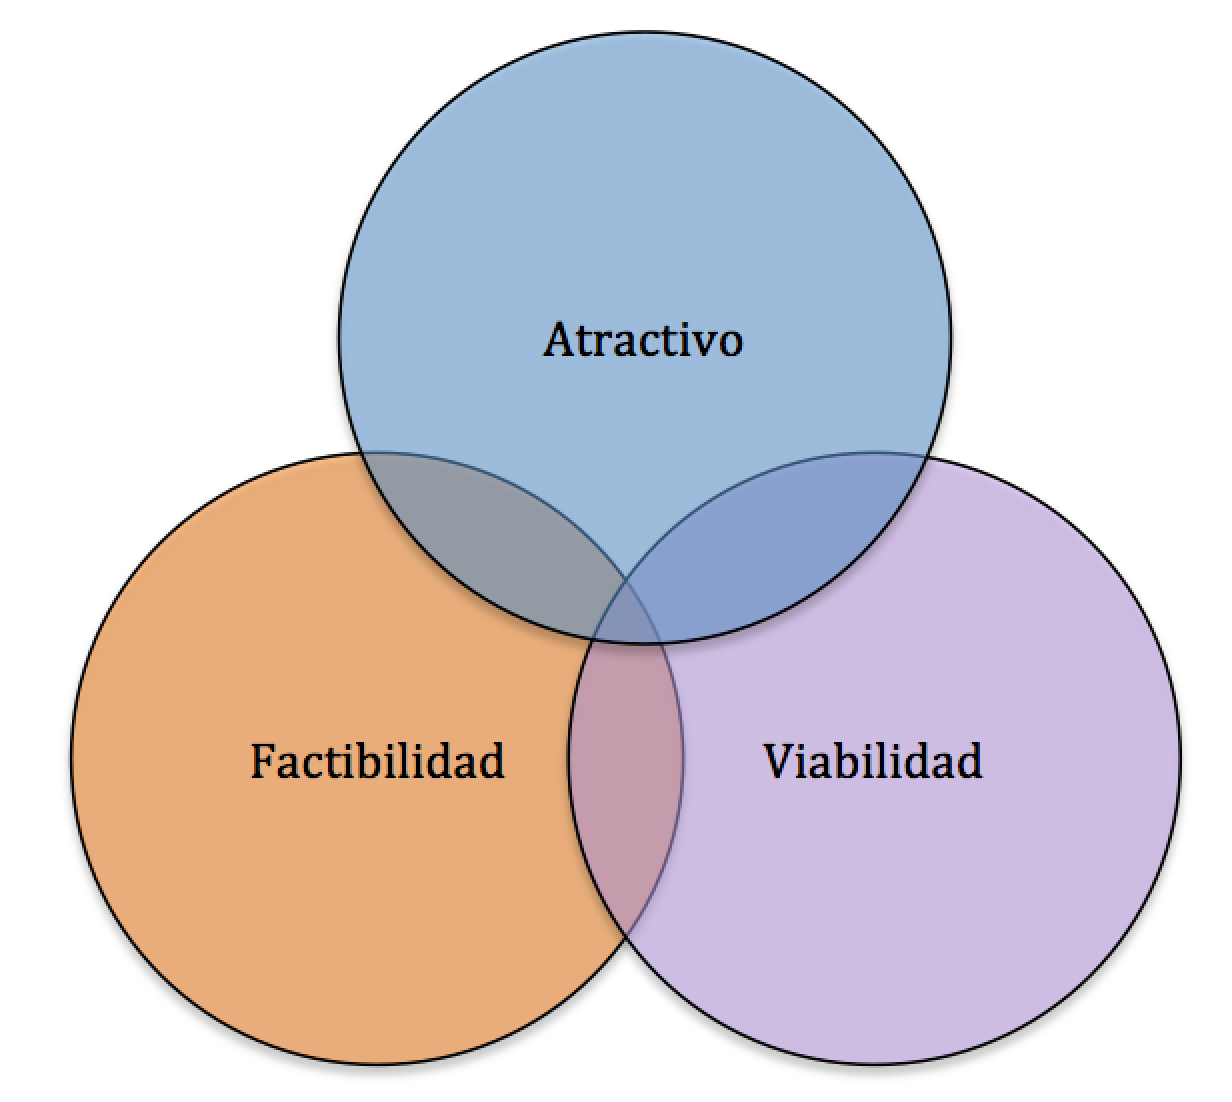
\includegraphics[width=0.7\textwidth]{3_burbujas}
\end{center}

Este es un modelo que aparentemente est\'a completo, y de hecho esta parece ser la forma en que muchos inventores enfocan su trabajo: abordando los tres aspectos simult\'aneamente usando un equipo multidisciplinario:

\begin{itemize}
\item Marketing trabaja en las pruebas de ``atractivo'' exponiendo a clientes conceptos y buscando retroalimentaci\'on.
\item Los ingenieros y los cient\'ificos se dirigen a los laboratorios para trabajar en prototipos para probar ``factibilidad''.
\item Los analistas crean hojas de c\'alculo para modelar la ``viabilidad'' bajo distintos escenarios.
\end{itemize}

Todo el mundo se siente productivo y el trabajo en general se muestra a los Inversionistas como un esfuerzo gratificante, coordinado y eficiente.
\\ \\
Yo prefiero pensar en estos puntos cr\'iticos como una secuencia:
    \begin{center}
    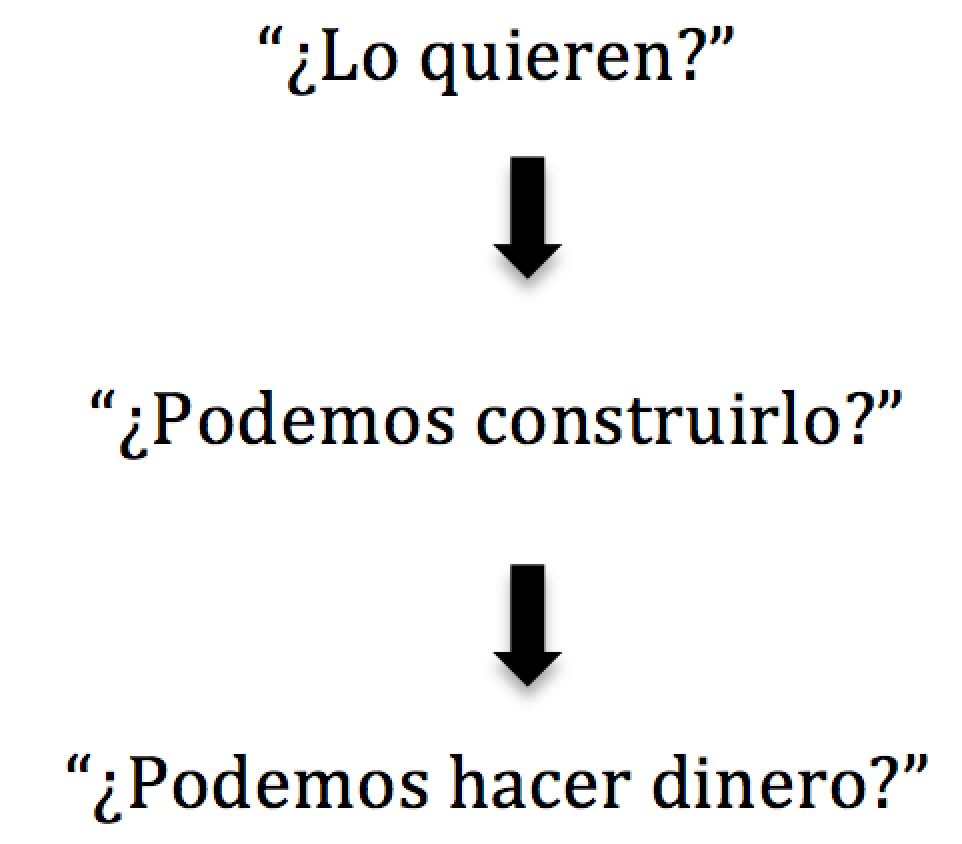
\includegraphics[width=0.4\textwidth]{3_preguntas}
    \end{center}

Para entender por qu\'e esta secuencia es muy importante, vamos a revisar en orden inverso. ``Podemos hacer dinero?'' Se relaciona con el modelo de negocio que los inventores planean realizar alrededor del nuevo producto. Tenemos el canal apropiado construido? Cu\'al es el modelo de monetizaci\'on, c\'omo se obtendr\'an beneficios? El nuevo producto canibalizar\'a el negocio existente?
\\ \\
Todo esto es muy importante para el \'exito final, pero irrelevante sin antes probar que el producto es posible de hacer.
\\ \\
``Podemos construirlo?'' Tiene que ver con la capacidad t\'ecnica, trae muchas inc\'ognitas por que suele ser la pregunta m\'as costosa y que requiere mas tiempo para ser respondida. Podemos hacer que sea confiable? Las pruebas fueron por el tiempo suficiente? Funcionar\'an las caracter\'isticas principales y trabajar en conjunto? Tenemos emocionantes colores / sabores / caracter\'isticas? Tenemos la materia prima / socios para negocios / proveedores bajo t\'erminos de mutuo beneficio? Y as\'i sucesivamente...
\\ \\
Una vez m\'as, cr\'itico a realizar, pero irrelevante a menos que los clientes quieran la soluci\'on.
\\ \\
``Lo quieren?'', tiene que ver con la demanda del mercado. Inventores creen que tienen una soluci\'on a una necesidad del mercado, sea o no del conocimiento del cliente o si a\'un no se ha establecido esa necesidad. La mayor\'ia de los Inventores trabajan bas\'andose en ideas indicativas sobre la demanda del mercado. Pretotyping propone una disciplina para la exploraci\'on de esta primera pregunta, proponiendo que sea la primera en la secuencia al ser reflexiva acerca de nuestras prioridades.
\\ \\
Para empezar, ``Lo quieren?'' tiene una serie de posibles variantes, dependiendo de la naturaleza del \textbf{\textit{it}} en cuesti\'on:

\begin{itemize}
\item Lo utilizar\'an en donde est\'an? (Ambiente, contexto).
\item Se adaptar\'an para poder usarlo? (Conducta, cambio).
\item Lo utilizar\'an si luce de esta manera? (Apariencia).
\item Lo utilizar\'an si hace/no-hace X? (Funcionalidad).
\item Lo comprar\'an de esta manera? (Canal).
\item Lo comprar\'an si cuesta mas que X? (Precio).
\end{itemize}

Recordemos IBM y su concepto Voz-a-Texto. Las preguntas a responder en su experimento pretotype incluyeron: ``Los clientes lo usar\'an?'', ``Lo van a usar para todo tipo de comunicaciones de la oficina?'' y "Lo usar\'an suficientes veces como para cambiar su actual soluci\'on (asignar un mecan\'ografo)?''.
\\ \\
O en el caso de Webvan, algunas de las preguntas ``Lo quieren?'' que \underline{debieron} haber incluido:

\begin{itemize}
\item ``Lo comprar\'an reiteradas veces?''
\item ``Los clientes, tanto de la ciudad como de los suburbios lo comprar\'an?''
\item  ``Qu\'e combinaci\'on de comestibles (por ejemplo, frescos vs envasados??) van a comprar con nosotros?''
\end{itemize}

Algunos avances convincentes desaf\'ian las probabilidades y tienen \'exito a pesar de que antes de ser lanzados no es claro que cumplan una necesidad para los clientes (El iPad de Apple es un ejemplo). Estos son pocos y distantes entre s\'i, sin embargo, y no pueden ser tomados como un indicador de infalibilidad (Lisa y Newton de Apple). La forma m\'as inteligente de jugar es dar prioridad a las pruebas de la demanda actual del mercado antes de hacer una gran inversi\'on.
\\ \\
Perm\'itanme presentar una nueva gram\'atica para la comunicaci\'on entre Inventor-Inversionista mediante enfoques pretotype, comenzando por la m\'as sencilla. Voy a incluir en algunos ejemplos de la vida real de historias de \'exito usando pretotyping para ilustrar las diferentes t\'ecnicas. Tenga en cuenta que el ``\'exito'' corresponde a un experimento exitoso, no necesariamente el \textbf{\textit{it}} correcto: no todos los productos en cuesti\'on se pusieron en marcha, pero en todos los casos la decisi\'on ``go/no-go'' se tom\'o de una manera r\'apida y barata.
\\ \\
TECNICAS PRETOTYPING
\\ \\
\begin{enumerate}
\item \textbf{El Pretotype Fake Door}
\\ \\
Fake Door\footnote{Creditos a Jess Lee de Polivore por el nombre Fake Door} (Puerta Falsa) es el punto de entrada para la comercializaci\'on de una idea a\'un sin desarrollar. Los inventores pueden crear una puerta falsa para la publicidad de un nuevo producto o servicio, luego se puede hacer seguimiento de la tasa de respuesta para ver qui\'en estar'ia interesado en el producto o servicio. La soluci\'on ni siquiera tiene que existir, sin embargo, una indicaci\'on inicial de inter\'es puede ser capturado a practicamente coste cero.
\\ \\
Las tecnolog\'ias Web permiten un metodo muy robusto que consiste en:

\begin{itemize}

\item Analizar las respuestas de los clientes a diferentes frases o palabras (usando anuncios en l\'inea vinculados a palabras de b\'usqueda espec\'ificas).

\item Links ubicados en sitios Web (los click que se han realizado).

\item Formularios sencillos (tales como pedir a los clientes para una direcci\'on de correo electr\'onico).

\end{itemize}

Fake Door no tiene que estar necesariamente basado en la web, correos electr\'onicos, carteles y otros medios pueden ser utilizados para simular la existencia de la soluci\'on.
\\ \\
Alberto cre\'o un Fake Door para probar la demanda de su libro \textit{Pretotype It}. Creyendo que sus probables lectores estar\'ian interesados en la innovaci\'on, contrat\'o AdWords para palabras relacionadas con el desarrollo y fases de prueba de la innovaci\'on, tales como \textit{prototyping}. \'El y yo hicimos lo mismo para nuestro reciente taller en Stanford Graduate School of Business creando un peque\~no folleto de invitaci\'on a la clase. En ambos casos, las respuestas que recibimos (clics a trav\'es de correo electr\'onico y solicitudes de informaci\'on adicional) alient\'o continuar con el desarrollo.

\begin{center}
    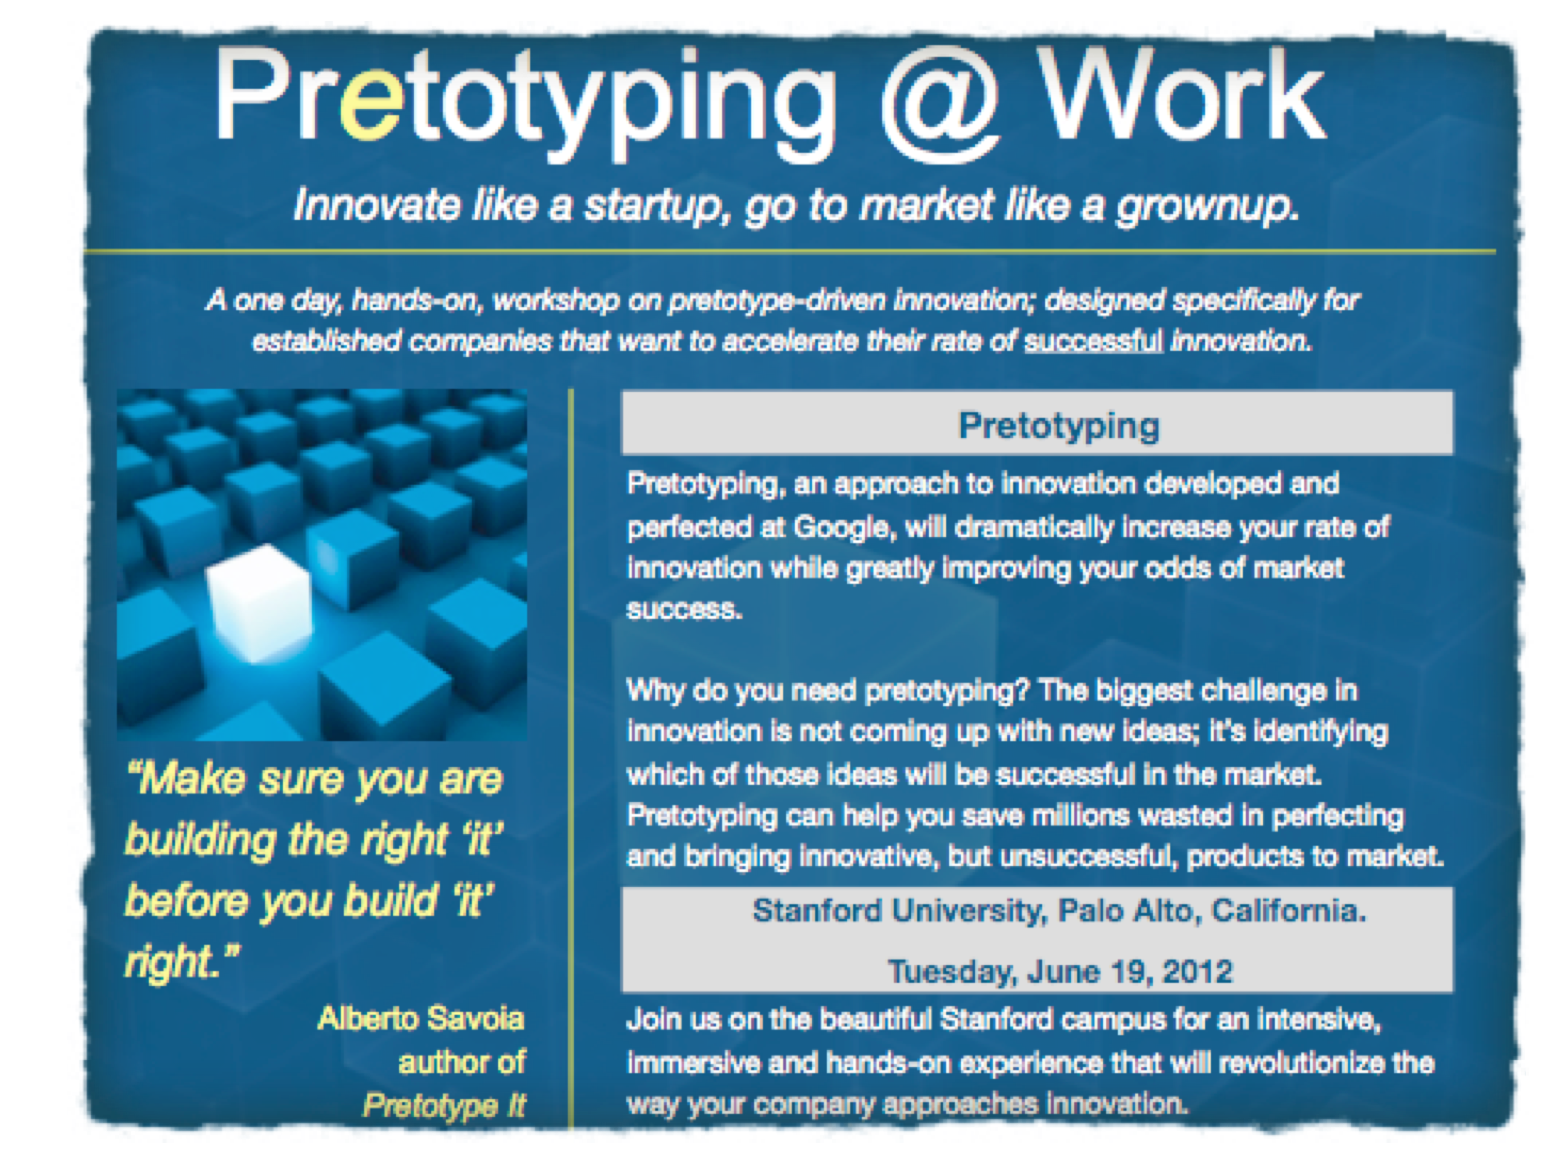
\includegraphics[width=0.8\textwidth]{folleto}
\end{center}

El pretotype Fake Door es generalmente el mas simple y la mejor opci\'on cuando se requiere testing del mercado. Considerar la utilizaci\'on de Fake Door cuando:

\begin{itemize}

\item Tu idea puede ser descrita y presentada a los potenciales clientes de manera concisa. El propietario de un restaurante podr\'ia poner un nuevo item, descrito y con precio al igual que todas las opciones actuales en el men\'u, de esta manera puede ver si los clientes se interesan. Un nutricionista puede colocar un anuncio en l\'inea que presenta su idea para una aplicaci\'on que proporciona una gu\'ia de selecci\'on de comida cuando la gente busca el t\'ermino ``comidas saludables''.

\item Usted est\'a seguro de que puede manejar las expectativas de los clientes entusiastas haciendo un seguimiento en un plazo adecuado. Al menos un fabricante de autom\'oviles ha desplegado un fake door antes de dise\~nar un nuevo modelo, lo que demuestra que algunos clientes pueden ser pacientes en efecto, por lo vale la pena pensar en el futuro!

\end{itemize}

\item \textbf{El Pretotype Pinocchio}
\\ \\
Como todos saben, Pinocchio es la marioneta de madera cuyos sue\~nos de convertirse en un ni\~no de verdad se hacen realidad gracias a la intervenci\'on de un hada. De esta manera, un pretotype Pinocchio corresponde a un artefacto inanimado (o ``tonto'') que act\'ua como aproximaci\'on al objeto real.
\\ \\
El Pretotype Pinocchio se inspir\'o en la historia del desarrollo de lo que mas tarde ser\'ia el Palm Pilot, el ic\'onico asistente personal digital (PDA) de la d\'ecada de los 90. Jeff Hawkins, fundador de Palm era un experto y evangelista en software de reconocimiento de escritura a mano y ten\'ia la esperanza de que la tecnolog\'ia pudiera revolucionar la organizaci\'on personal. Su experiencia con el previo lanzamiento de una computadora de mano, el GRiDPad, le dej\'o una lecci\'on: la revista Time llam\'o el dispositivo ``una maravilla de la ingenier\'ia, pero un fracaso en el mercado debido a que (en palabras de Hawkins) era demasiado grande''.
\\ \\
Hawkins estaba decidido a no repetir el error, y se concentr\'o en el factor forma de su nuevo dispositivo. Ten\'ia un tama\~no y forma en mente: deb\'ia entrar en un bolsillo de la camisa. La soluci\'on de Hawkins fue cortar un bloque de madera para adaptarlo a su bolsillo de la camisa y luego cubrirla con un papel con la imagen de una interfaz sencilla (ver imagen, al lado el dispositivo acabado).

\begin{center}
    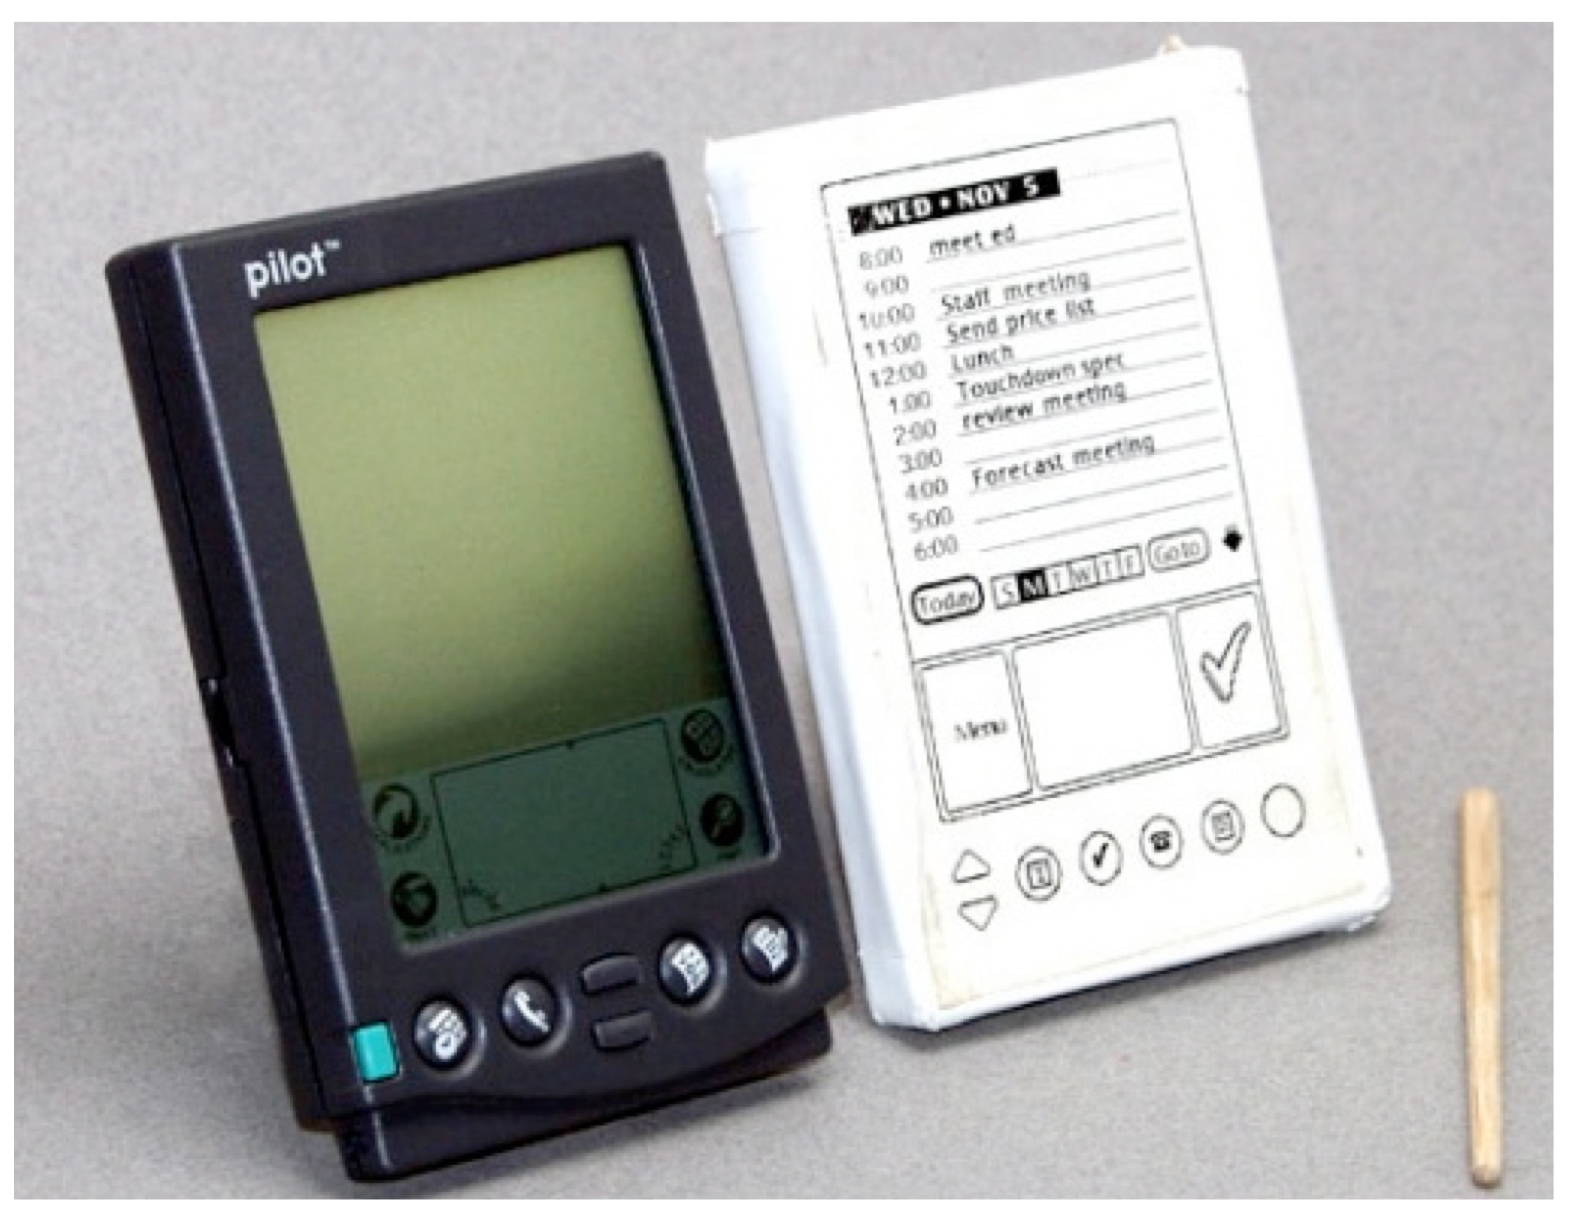
\includegraphics[width=0.8\textwidth]{palm_pilot}
\end{center}

Anduvo con \'el por varias semanas, fingiendo que era una computadora en funcionamiento, imitando sus interacciones cuando \'el encontraba una necesidad dentro de sus funciones imaginadas. Por ejemplo, si recibi\'o una invitaci\'on para el almuerzo, sacaba el bloque del bolsillo y se pretend\'ia revisar su calendario para la fecha propuesta, entonces ``guardaba'' el evento con su ``stylus'' que era un peque\~no palo que llevaba consigo.
\\ \\
Hawkins, no solo fue dram\'atico realizando su experimento, si no que tambi\'en valido su teor\'ia sobre el valor del factor de forma y adem\'as le dio una idea de las funciones m\'as \'utiles. Las cuatro funciones que Hawkins m\'as us\'o durante el experimento (calendario, libreta de direcciones, lista de tareas y tomar notas) fueron las que inclu\'ia el Pilot al momento del lanzamiento.
\\ \\
Empresas de dise\~no emplean regularmente Pinocchios para conseguir una buena sensaci\'on para los atributos cr\'iticos, un buen ejemplo es el disector quir\'urgico Diego, dise\~nado por IDEO. Para poner a prueba la capacidad de un cirujano para equilibrar, posicionar y controlar con precisi\'on la herramienta, el equipo recurri\'o a la oficina de suministros e insumos para comprender los requisitos que requieren cirug\'ias realizadas con una sola mano.

\begin{center}
    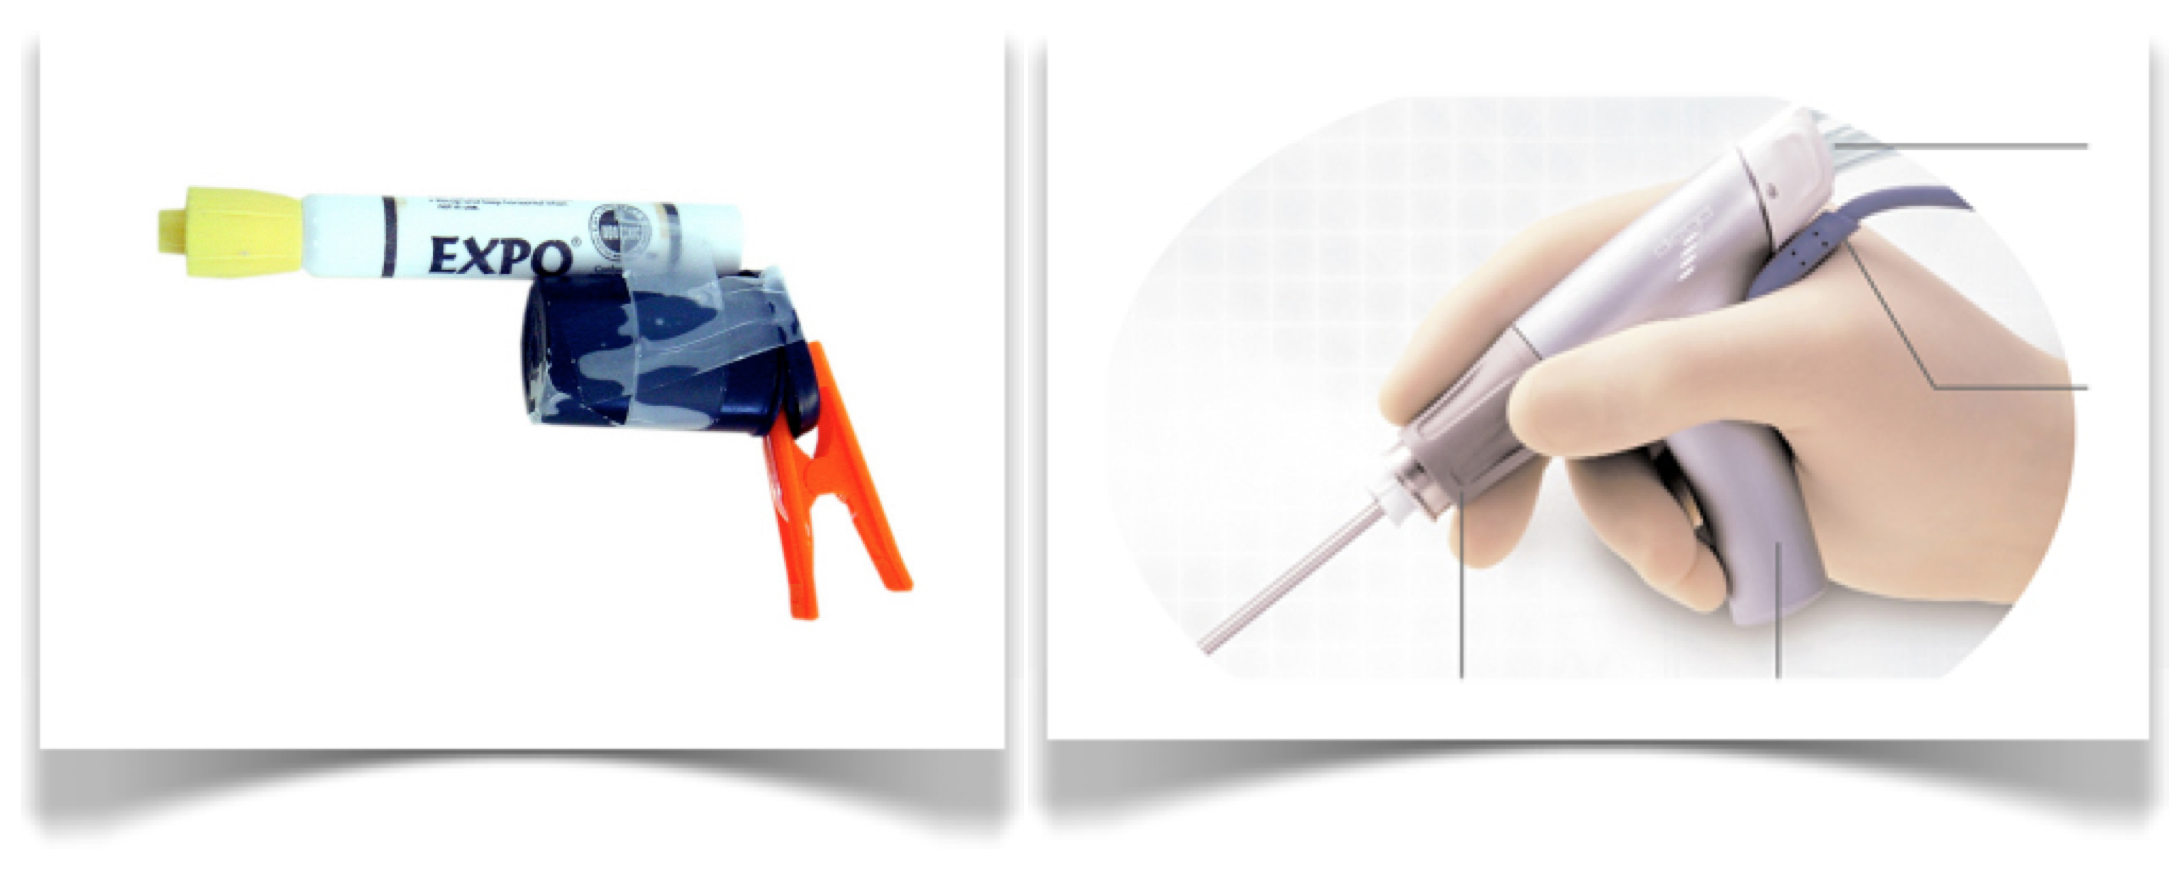
\includegraphics[width=1.0\textwidth]{diego}
\end{center}

Considerar un Pretotype Pinocchio cuando:

\begin{itemize}

\item La soluci\'on requiere un cambio \textit{significativo} o de \textit{adaptaci\'on} por parte de los clientes para desarrollar un nuevo h\'abito (por ejemplo, el uso de una nueva aplicaci\'on), aprender una nueva forma de control (por ejemplo, los movimientos del dedo en tel\'efonos inteligentes o manejar un Segway) o simplemente abandonar un soluci\'on existente.

\item Se espera que la demanda sea sensible a la \textit{apariencia} o \textit{factor de forma} de la soluci\'on, tambi\'en ayuda a testear rangos de tama\~no, formas, pesos, materiales, etc.

\end{itemize}

\item \textbf{Pretotype The Mechanical Turk}
\\ \\
El Mechanical Turk era un jugador de ajedrez ``aut\'omata'', dise\~nado a finales del siglo 18 por un cortesano h\'ungaro que intent\'o impresionar a la Emperatriz de aquella \'epoca. El dispositivo pod\'ia ser abierto para revelar un complejo trabajo de relojer\'ia que aparentemente manejaba el brazo izquierdo de un maniqu\'i compuesto de cabeza y hombros (el Turco) que se encontraba sobre el dispositivo. El fabricante desafiaba a un miembro de la audiencia para jugar contra el Turco.
\\ \\
 La ilusi\'on fue posible gracias a un escondite h\'abilmente disimulado dentro del dispositivo, donde un jugador de ajedrez humano pod\'ia ``ver'' los movimientos hechos por su oponente por medio de imanes que cambiaban de posici\'on en respuesta a las piezas que se mov\'ian sobre la superficie del tablero de ajedrez. Para lograr que el aut\'omata se moviera, el jugador (de mucho en el talento aunque de de baja estatura) operaba un arreglo de palancas al estilo pant\'ografo conectado al brazo del Turco. Con esta mec\'anica era posible agarrar, mover y soltar las piezas sobre el tablero de la mesa.
 \\ \\
 El pretotype Mechanical Turk\footnote{Tambi\'en conocido como la t\'ecnica  ``El Mago de Oz'' o ``El Paradigma de Oz'', llamado as\'i por el Dr. John Kelley para describir sus m\'etodos de experimentos psicol\'ogicos en la Universidad Johns Hopkins en los a\~nos 70 y 80.} entonces simula sofisticada tecnolog\'ia que ser\'ia costosa o que requiere mucho tiempo para construir desde cero. Es por esto que se usa el poder humano para sustituir a la tecnolog\'ia. Un test Mechanical Turk bien dise\~nado proporciona a los clientes objetivo la experiencia b\'asica de una nueva propuesta tecnol\'ogica con una fracci\'on de la inversi\'on de desarrollo necesario.
 
 \begin{center}
    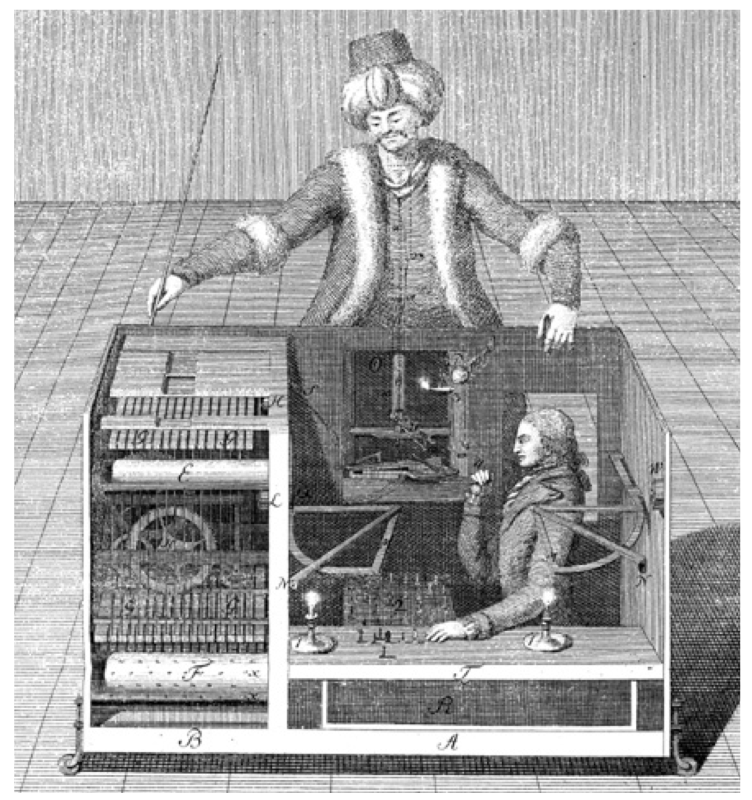
\includegraphics[width=0.6\textwidth]{mechanical_turk}
\end{center}
 
 El Pretotype Voz-a-Texto de IBM es un ejemplo magn\'ifico; El mecan\'ografo humano simulando el hardware y software a testear, exactamente como el peque\~no jugador de ajedrez en el Mechanical Turk hizo el papel de cerebro maestro del dispositivo.
 \\ \\
 Considerar el Pretotype Mechanical Turk cuando:
 
 \begin{itemize}
 
 \item Cuando el producto final requiere el desarrollo de una tecnolog\'a costosa y compleja, cuyas acciones y resultados podr\'ian ser simulados por los seres humanos.
 
 \item El valor de la soluci\'on depende de \textit{m\'ultiples elementos tecnologicos que interact\'uan.}
 
 \end{itemize}
 
 \item \textbf{El Pretotype One Night Stand}
 \\ \\
 El Pretotype One Night Stand (levantar en una noche) es un modelo en el que un servicio interactivo se presenta de una manera bastante completa  pero sin los detalles de infraestructura que requiere una soluci\'on permanente. Las instalaciones f\'isicas (espacio, equipos, accesorios, decoraci\'on) se pueden alquilar y ser presentadas como un ``set de Hollywood'' mientras dure la prueba y luego se desarma y todo es devuelto.
 \\ \\
Best Buy, un antiguo cliente m\'io, ten\'ia una idea para un nuevo servicio. La idea era ver si los clientes podr\'ian ser alentados a comprar nuevos gadgets electr\'onicos como c\'amaras de video y televisores ofreciendo alg\'un valor simb\'olico para sus art\'iculos usados en buen estado. Este concepto  se llam\'o NextPlay, la soluci\'on completa consist\'ia de un departamento dentro de la tienda que recib\'ia a los clientes, comprobaba si los art\'iculos eran funcionales y finalmente se le ofrec\'ia al cliente un cr\'edito para una nueva compra con una tarjeta con el valor almacenado. Podr\'ia esto ser probado a bajo costo?
\\ \\
El test Pretotype consisti\'o en una tienda de campa\~na en el estacionamiento de una tienda Best Buy en Boca Raton, FL. La tienda de campa\~na cubri\'o un espacio temporal de trabajo compuesto por mesas plegables, una extensi\'on de poder de la tienda y un peri\'odico de art\'iculos usados. Parte de la publicidad del servicio se mostr\'o en un peri\'odico local una semana antes de la prueba. El test se realiz\'o un fin de semana: la gente trajo videoc\'amaras usadas??, televisores y celulares; los que fueron probados por el equipo. Los clientes que trajeron alg\'un producto que el equipo consider\'o que tuviera vida \'util, se les pag\'o en cr\'edito de la tienda seg\'un el peri\'odico de art\'iculos usados.

\begin{center}
    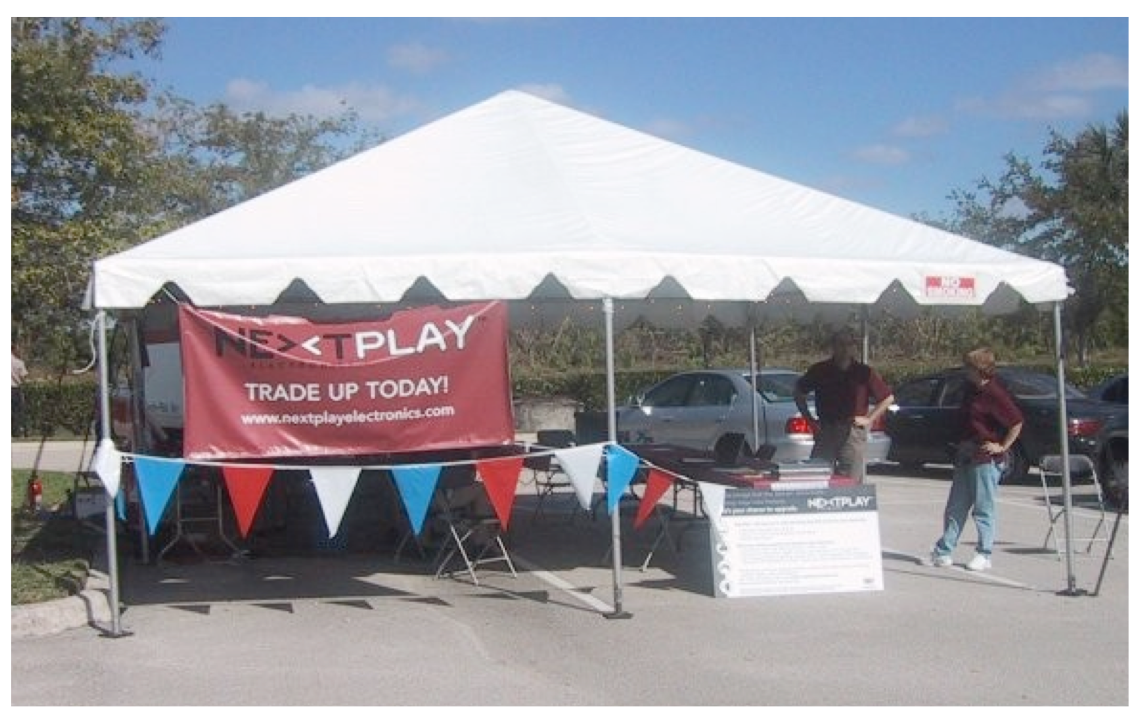
\includegraphics[width=0.8\textwidth]{best_buy}
\end{center}

El punto de venta de la tienda (POS) permiti\'o al equipo realizar seguimiento sobre que tarjetas se utilizaron como parte de una compra posterior. No s\'olo eso, los datos tambi\'en mostraron si la tarjeta fue cobrad\'a inmediatamente (en la mayor\'ia de los casos, s\'i) y tambi\'en se identific\'o el promedio de gasto extra sobre cada tarjeta.
\\ \\
Hoy en d\'ia, esta soluci\'on se conoce como Technology Trade-In, y esta funcionando en muchas tiendas. El servicio ha experimentado una considerable evoluci\'on y desarrollo - por ejemplo, en la actualidad la soluci\'on opera en Best Buy pero es administrada por un partner - Lo importante ac\'a es que la validaci\'on inicial del concepto se llev\'o a cabo de forma r\'apida y barata en un estacionamiento.
\\ \\
Una variante interesante del One Night Stand es el Pretotype Provincial. Provincial implica simplemente exponer la oferta Pretotype a un subconjunto limitado de mercados y clientes.
\\ \\
Considerar el pretotype One Night Stand o Pretotype Provincial cuando:

\begin{itemize}

\item La soluci\'on es - o depende cr\'iticamente de - una forma de \textit{experiencia interactiva de servicio.}

\item Se espera que la demanda de la oferta var\'ie significativamente de un mercado a otro.

\item Se espera que la demanda de la oferta ser\'a sensible a la elecci\'on del \textit{canal} por lo que se necesita poner a prueba una serie de posibles puntos de intercepci\'on de los clientes.

\end{itemize}

\item \textbf{El Pretotype Impersonator}
\\ \\
Un Pretotype Impersonator (Imitador) es uno donde un producto o servicio existente obtiene una nueva envoltura o ``piel'' con el fin de hacerse pasar por una nueva oferta a testear. Esto tiene la ventaja de que el producto existente tiene caracter\'isticas de rendimiento conocidas, por lo tanto esta informaci\'on puede ser utilizada cuando se pone en las manos de los clientes de prueba.
\\ \\
Piense en una nueva idea de un producto alimenticio, algo como una comida preparada o un trago. Un producto existente en la misma o categor\'ia similar podr\'ia ser re-envasado para hacerse pasar por la nueva oferta. Dado que los inventores a\'un est\'an respondiendo la pregunta ``Lo quieren?'', la capacidad de probar la selecci\'on actual mediante la compra de un producto equivalente es todo lo que Impersonator requiere. Pruebas de gusto, incluyendo preferencias de sabor, tama\~no de la porci\'on, etc, deben esperar hasta m\'as tarde en el proceso.
\\ \\
Un excelente ejemplo de Impersonator viene de Tesla Motors. El a\~no 2003, los fundadores de Tesla ten\'ian una ambiciosa idea (un autom\'ovil el\'ectrico de 2 puertas deportivo) y un desaf\'io de marketing (Tesla era un desconocido como fabricante de autom\'oviles). Con el fin de convencer a los potenciales compradores de adquirir su coche, Tesla cre\'o un pretotype de lo que el coche ser\'ia.
\\ \\
La base para el Pretotype fue Lotus Elise, el coche cuya tecnolog\'ia de chasis fue finalmente licenciada - y muy modificada - por Tesla para proporcionar la base para el chasis del Roadster. Lotus suministr\'o a Tesla un Elise ``hueco''- un coche sin un tren de potencia - que estaba lleno de componentes clave como bater\'ias y motores de CA. Esto fue no un prototipo, el veh\'iculo no funcionaba, sin embargo, con una inversi\'on (relativamente) baja, Tesla fue capaz de demostrar a los compradores una aproximaci\'on muy cercana del dise\~no final.

\begin{center}
    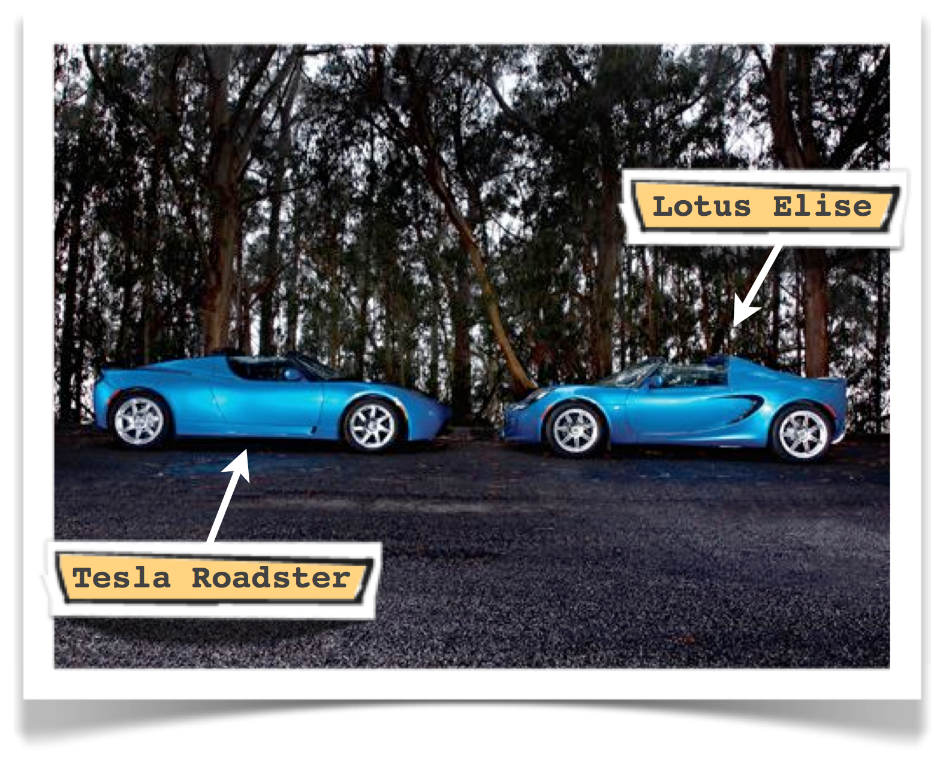
\includegraphics[width=0.9\textwidth]{tesla}
\end{center}

Como si esto fuera poco astuto, Tesla tambi\'en despleg\'o un pretotype Fake Door para validar a\'un m\'as la demanda. En vez de quedarse en Thoughtland, Tesla fue mas all\'a preguntandole a sus potencial clientes ??si comprarian Roadster'' construido por ellos. Finalmente se pregunt\'o: ??Est\'a dispuesto a dejar un dep\'osito de \$ 5.000 para garantizar una fecha de entrega?''. Este es un verdadero test de preferencia, del que Tesla consigui\'o varios cientos de dep\'ositos, un resultado que claramente tranquiliz\'o a los inversores.
Variaciones del Pretotype Impersonator incluyen:
\begin{itemize}
\item The Infiltrator (El Infiltrado), el inventor cambia la finalidad un producto existente cambiandolo sigilosamente o agregando una o m\'as caracter\'isticas nuevas, por ejemplo, las pruebas A / B de diferentes dise\~nos de p\'aginas web.
\item El Pretend-To-Own (pretender tener), en el que el inventor utiliza leasing o arrienda equipos en vez de comprarlos, por ejemplo, el alquiler de un n\'umero peque\~no de Toyota Prius para realizar un test pretotype a un servicio de alquiler de coches ecol\'ogicos.
\item The Teaser (la intriga), en el que el inventor crea un subconjunto totalmente funcional de la soluci\'on completa, por ejemplo, los primeros 3 cap\'itulos de una novela o los 10 primeros minutos de una pel\'icula.

\end{itemize}

Considerar los pretotype Impersonator, Infiltrator, Pretend-To-Own o Teaser cuando:

\begin{itemize}
\item Una test para valorar la soluci\'on depende de la \textit{capacidad de los clientes para interactuar con un dise\~no a gran escala} y que necesita un sustituto plausible para el tama\~no, forma, color, caracter\'isticas, etc de la soluci\'on.
\end{itemize}


\item \textbf{El Pretotype Minimum Viable Product (MVP)}
Un MVP\footnote{El t\'ermino MVP fue creado por Eric Ries, autor de \textit{The Lean Startup.}} es la transici\'on de pretotyping a prototipos del eventual producto. A veces es necesario invertir un cierto nivel de esfuerzo en la creaci\'on de un prototipo funcional, un artefacto que entregue las funciones principales de la soluci\'on completa que mas adelante se pondr\'a en manos de los clientes. La caracter\'istica clave del MVP es que el artefacto sea el prototipo \textit{m\'as simple posible}, reduciendo todo hasta el m\'inimo requerido para llevar a cabo la prueba en directo, todo esto sin adornos adicionales, de tal manera que el menor n\'umero de variables sea puesta bajo an\'alisis en cualquier momento.
\\ \\
Considerar el Pretotype MVP cuando:

\begin{itemize}
\item Usted ha aprendido todo lo posible acerca de la demanda del mercado usando pretotypes simples (Fake Door, Pinocchio, Mechanical Turk, One Night Stand o Impersonator) pero es necesario lograr \textit{mayor comprensi\'on, por lo que se requiere una mayor interacci\'on con el cliente con un artefacto en funcionamiento.}
\end{itemize}

\centerline{--------------------------------------------------------}

\end{enumerate}

Estos 6 modelos y sus variantes constituyen un conjunto de \textit{bloques de Lego} con los cuales se comenzar a experimentar con pretotyping\footnote{La hoja de trabajo PretoStorming en el Ap\'endice 1 se puede utilizar para ayudarle a dise	~nar pruebas pretotype, desde identificar preguntas como ``lo quieren?'' hasta un peque\~no plan de negocios.}. Estoy constantemente aprendiendo sobre nuevas variantes que podr\'ian merecer su propia etiqueta y usted puede descubrir m\'as en el camino. Mi consejo es centrarse menos en la etiqueta y enfocarse en desafiar a su equipo para encontrar un pretotype cada vez mas simple.

\subsection{Una llave en la caja de herramientas de la innovaci\'on}

Inventores con estudios en herramientas de innovaci\'on a menudo preguntan a dos cosas:

\begin{itemize}

\item ``C\'omo es  Pretotyping diferente de un prototipo?''
\item ``No es Pretotyping solo otro nombre para <<{\textit{inserte el nombre de de una herramienta para la innovaci\'on}}>>?''

\end{itemize}

En el primer caso, la confusi\'on se debe a que los inventores han sido entrenados para usar ``prototipo'' como un t\'ermino general para cualquier tipo de experimentaci\'on entre la idea y el producto terminado. Piense en los tableros de conceptos, esquemas, formas moldeadas o talladas, dispositivos a medio construir, y simulaciones que ha presenciado durante su carrera: la mayor\'ia ha tenido la etiqueta de ``prototipo''. Se ha convertido en un t\'ermino que puede referirse a cualquier simulacro no-finalizado del \textbf{\textit{it}} final.
\\ \\
En este contexto, espero que ``Pretotyping'' pueda aislar convenientemente,  el hiper-simplificado uso extremo de la palabra ``prototipo'':

\begin{itemize}

\item Un Pretotype pone a prueba la pregunta ??Lo quieren?''. El horizonte temporal es de horas o d\'ias, y el entreg\'able principal son los datos de la demanda.

\item Un prototipo pone a prueba la pregunta ``Podemos construirlo?''. El horizonte temporal es a menudo meses o a\~nos y el entreg\'able principal es un artefacto funcional que valida uno o m\'as atributos de rendimiento.

\end{itemize}

En el caso de la segunda pregunta, los inventores a menudo piensan que ya est\'an utilizando Pretotype bajo la apariencia de otra etiqueta, tales como como \textit{la Voz del Cliente, investigaci\'on etnogr\'afica, entrevistas para causar empat\'ia, etc.} Estas t\'ecnicas pueden ser \'utiles para identificar problemas con las ofertas actuales o las oportunidades para nuevas ofertas: en otras palabras, se aplican antes de la idea (Pre-idea). Algunos inventores creen que ya est\'an utilizando pretotyping cuando lo aplican despu\'es de la idea (Post-idea). Estas t\'ecnicas son menos eficaces que pretotyping porque no ofrecen una verdadera prueba de la preferencia presentada al cliente. En resumen:

\begin{itemize}

\item \textbf{Pre-idea:} T\'ecnicas de conocimiento del cliente, tales como \textit{VOC} pueden ser \'utiles en la estimulaci\'on de ideas para nuevos productos y servicios, mediante la revelaci\'on de las frustraciones de los clientes, necesidades o ambiciones no cumplidas.

\item \textbf{Post-idea:} Pretotype re\'une aut\'enticos datos de la demanda del mercado presentando opciones de preferencias a los clientes y la b\'usqueda de compromisos para adquirir el producto. Otras t\'ecnicas como \textit{grupos de enfoque} utilizan una abstracci\'on de la idea del producto, por lo general en la forma de un concepto presentado a un cliente existente, que puede sesgar el an\'alisis, ya que se piden opiniones m\'as que compromisos.

\end{itemize}

El siguiente gr\'afico muestra por que yo considero que pretotyping corresponde a a la herramienta ``front-end de la innovaci\'on'' (o FEI\footnote{Esto es una simplificaci\'on para la exposici\'on, las personas encargadas del proceso de innovaci\'on tendr\'an algunas cr\'iticas reflexivas respecto a elementos faltantes. Por ejemplo, yo siempre recomiendo ``lentes'' adicionales para complementar informaci\'on sobre el cliente (por ejemplo, an\'alisis de las principales tendencias, ortodoxias o an\'alisis de puntos ciegos) y por supuesto, la verdadera naturaleza de FEI es iterativa.})  m\'as r\'apida y que mas ayuda a escapar de Thoughtland:

\begin{center}
    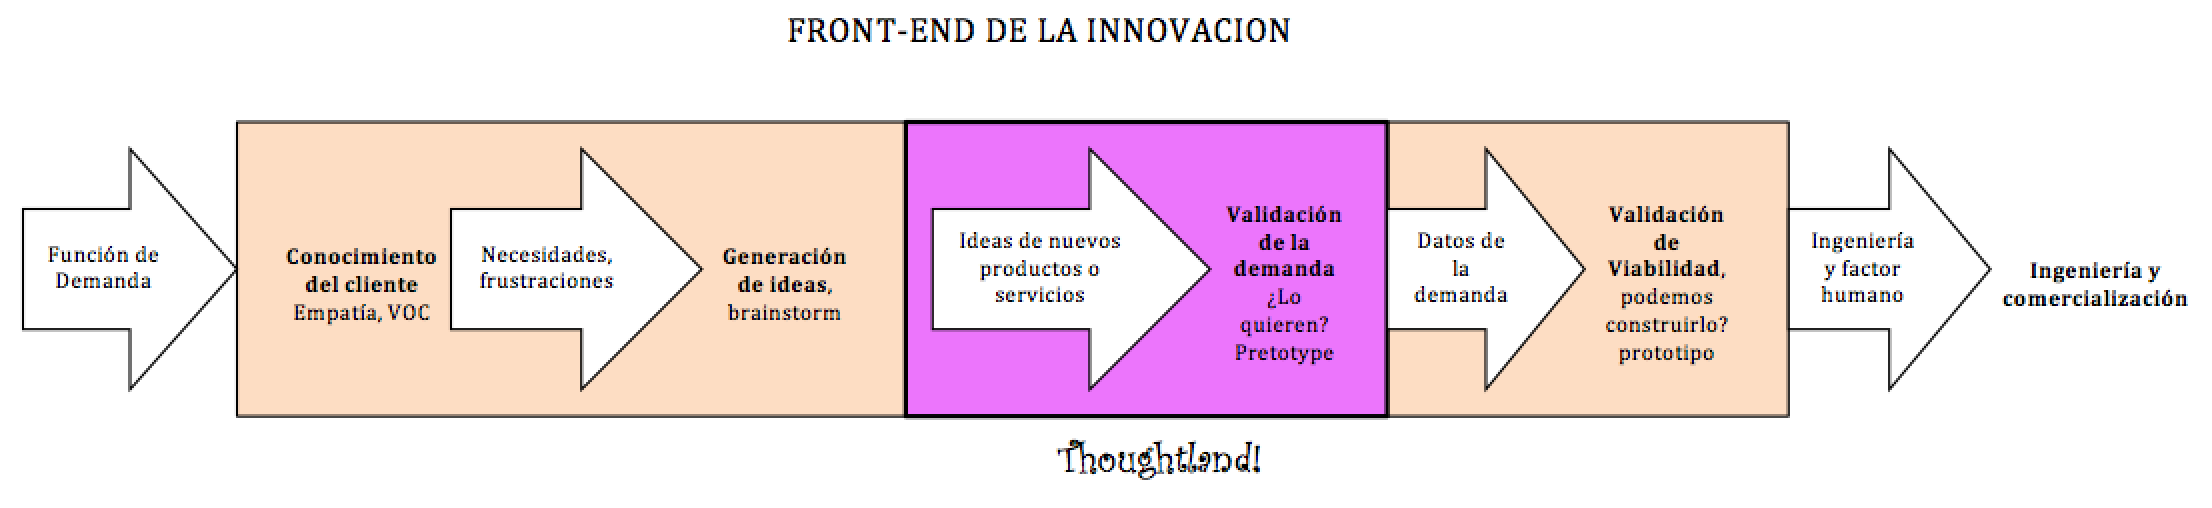
\includegraphics[width=1.1\textwidth]{frontend}
\end{center}

Tenga en cuenta que los Grupos Focales no desempe\~nan ning\'un papel en la validaci\'on de la demanda: simplemente creo que Pretotyping es una tecnolog\'ia superior y desplaza estas opiniones-intercambios de los mercados.

\clearpage
\section{INVIERTE COMO UN ADULTO}

Inversionistas, les ha pasado esto? Un equipo Inventor presenta una nueva idea: va a ser ENORME, REDEFINIR\'A LA INDUSTRIA, generar\'a ENORMES UTILIDADES!
\\ \\
Usted es esc\'eptico pero a\'un as\'i les da el espacio para investigar el potencial de mercado. Semanas m\'as tarde, el equipo reporta nuevamente.
\\ \\
Qu\'e han hecho? Los inventores han bosquejado un prototipo, ejecutaron grupos focales y construyeron una excelente proyecci\'on y estudio de este de negocio. Champ\'an virtual por todas partes y el equipo obtiene la siguiente etapa de financiamiento. Meses m\'as tarde, despu\'es de incluso m\'as esfuerzo de I + D y marketing, el proyecto se derrumba, mientras usted ofrece gracias no sinceras por los esfuerzos realizados. \textit{Usted lo sab\'ia!}
\\ \\
Por qu\'e ocurre esto? Porque los inventores no corren los mismos riesgos que los emprendedores o empresarios; Es el dinero de la empresa, y, francamente, a todos nos encanta trabajar en Thoughtland. A pesar de que su funci\'on incluye patrocinio de la innovaci\'on, en la pr\'actica usted es recompensado ??por su astuta administraci\'on de los negocios actuales.
\\ \\
Como lograr que los inventores piensen de manera diferente? Discuta las Leyes del Fracaso con ellos y rechace la euforia de Thoughtland. Acepte solo la evidencia de demanda que le dar\'ia la confianza suficiente para proceder y exija saber cual es el Pretotype que esta entregando estos datos. Repita.

\subsection{No lo crea, demuestrelo}

Ley presume que una persona acusada de un delito es inocente hasta que se demuestre su culpabilidad. De esta manera se protegen los derechos individuales.
\\ \\
Las Leyes de Fracaso indican que lo contrario debe aplicarse a las ideas en Thoughtland: un nuevo producto se considera un fracaso hasta que su probable \'exito pueda ser demostrado. De esta manera, se protegen los recursos de innovaci\'on limitados. 
\\ \\
A riesgo de volverme repetitivo, las opiniones en Thoughtland son rumores y realizar preguntas hipot\'eticas, como ``esta dispuesto?'', llama a la especulaci\'on. Lo qu\'e las ideas necesitan son \textit{pruebas en forma de datos.} Pretotype entrega datos.
\\ \\
Este cap\'itulo describe dos m\'etricas con las que los inventores y los inversores pueden construir progresivamente la confianza en las nuevas ideas, todo esto basado en datos.
\\ \\
RETORNO DE LA INVERSION PRETOTYPING (RPI)
\\ \\
RPI\footnote{En las Hojas de Trabajo I y II, en el ap\'endice 1, las m\'etricas pueden enmarcar la discusi\'on en torno a los objetivos de ajuste para el seguimiento ILI y OLI para las pruebas Pretotype.} proporciona la primera garant\'ia de que la validaci\'on de mercado para la nueva idea se puede lograr a bajo esfuerzo. RPI muestra la \textit{eficiencia en el aprendizaje} logrado al probar una idea mediante un experimento Pretotype en vez de un prototipo tradicional.
\\ \\
La eficiencia en el aprendizaje se puede expresar en cualquier unidad de tiempo (velocidad de aprendizaje) o dinero (costo de aprendizaje). Esta es la f\'ormula:

\begin{center}
    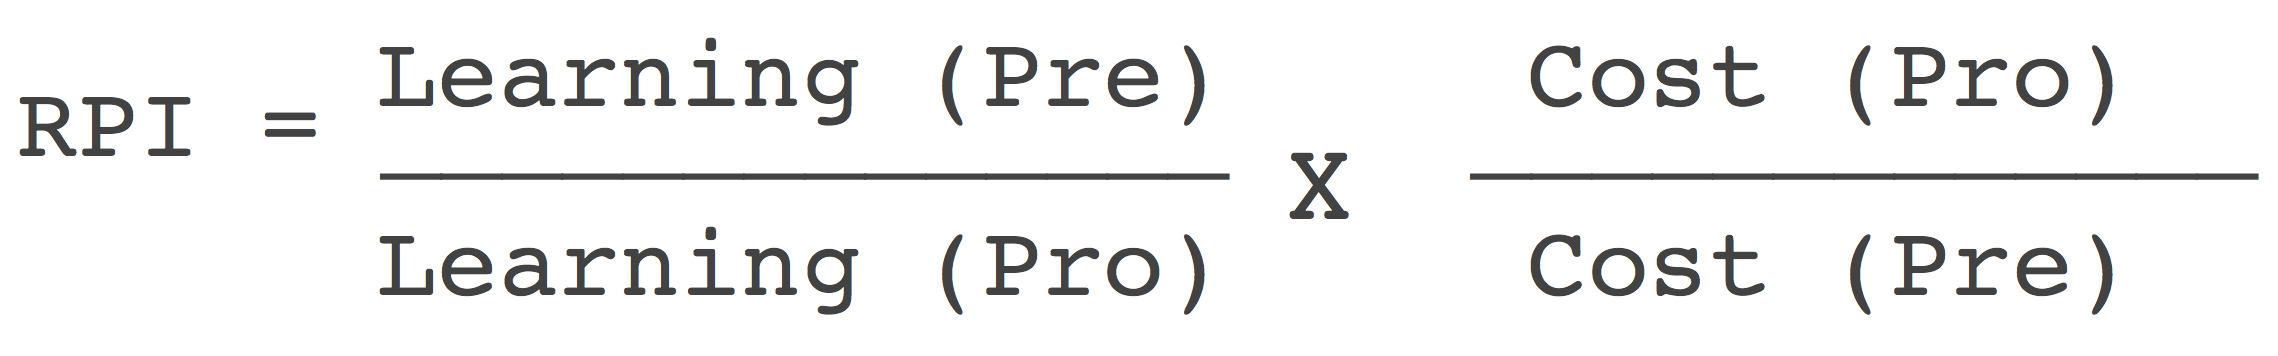
\includegraphics[width=0.9\textwidth]{RPI}
\end{center}

Donde:
\\ \\
Learning (Pre):		Cu\'anto (\%) cree que va a aprender de un Pretotype dado en comparaci\'on con el producto completo.
\\ \\
Learning (Pro):		Cu\'anto (\%) va a aprender de un prototipo o producto final - se ajusta al 100\% para el producto final.
\\ \\
Cost (Pro):		Cu\'anto costar\'ia (tiempo o \$) desarrollar/testear/publicitar un prototipo o producto final.
\\ \\
Cost (Pre):		Cu\'anto costar\'ia (tiempo o \$) para crear y probar un Pretotype dado.
\\ \\
Mostremos un ejemplo para ilustrar RPI, recordando a nuestros viejos amigos, Webvan; hagamos cuenta que somos los inventores e inversores detr\'as de Webvan. Tenemos esta idea estupenda que aparentemente va a significar un capital importante para el desarrollo: el plan de negocios requiere \$ 1B para construir completamente nuestra infraestructura. Ay! Si tuvi\'eramos m\'as confianza en la demanda del mercado. Antes de que podamos calcular RPI, tenemos que dise\~nar el Pretotype correcto.
\\ \\
Qu\'e ``es lo que quieren?'' Estas preguntas debemos responder (antes de gastar \$ 100M +)

\begin{itemize}

\item Que \% de personas utilizar\'a internet para comprar alimentos?
\item Que tan seguido lo utilizar\'an?
\item Las personas en la ciudad utilizar\'an mas el servicio que en los suburbios?
\item Que productos comprar\'an?
\item Cual en monto en dinero de una transacci\'on promedio?

\end{itemize}

Qu\'e dise\~no Pretotype nos dar\'ia buenos datos sobre estas preguntas? El lugar m\'as simple para empezar ser\'ia una campa\~na Fake Door, aunque dado que el acceso a la tecnolog\'ia es una parte cr\'itica de la soluci\'on de Webvan, lo siguiente suena mejor:

\begin{itemize}

\item Crear una pagina web de alta calidad (un front-end pulido sin back-end).
\item Promocionar localmente en una ciudad importante (por ejemplo San Francisco) y un suburbio (por ejemplo Palo Alto).
\item S\'i/cuando los pedidos comienzan a llegar, comprar comida en las tiendas existentes.
\item Arrendar camiones de entrega y contratar personal temporal para realizar las entregas.
\item Ejecutar el experimento por 4 semanas.

\end{itemize}

Debemos conseguir un fuerte indicador de la demanda de esta prueba, pero qu\'e proporci\'on va a ser parte del aprendizaje que se puede conseguir a partir de la construcci\'on de la soluci\'on completa? Para calcular el RPI, tenemos que hacer algunos c\'alculos sobre la eficacia que tendr\'ia este Pretotype MVP/Mechanical Turk. Se requiere objetividad, aunque el Pretotype se siente robusto: digamos 75\%. El coste del Pretotype tambi\'en requiere objetividad, pero teniendo en cuenta el costo de la soluci\'on completa, podemos ser generosos: \$ 1M.
\\ \\
Al incluir estos n\'umeros en la f\'ormula, el costo RPI de este Pretotype es:

\begin{center}
    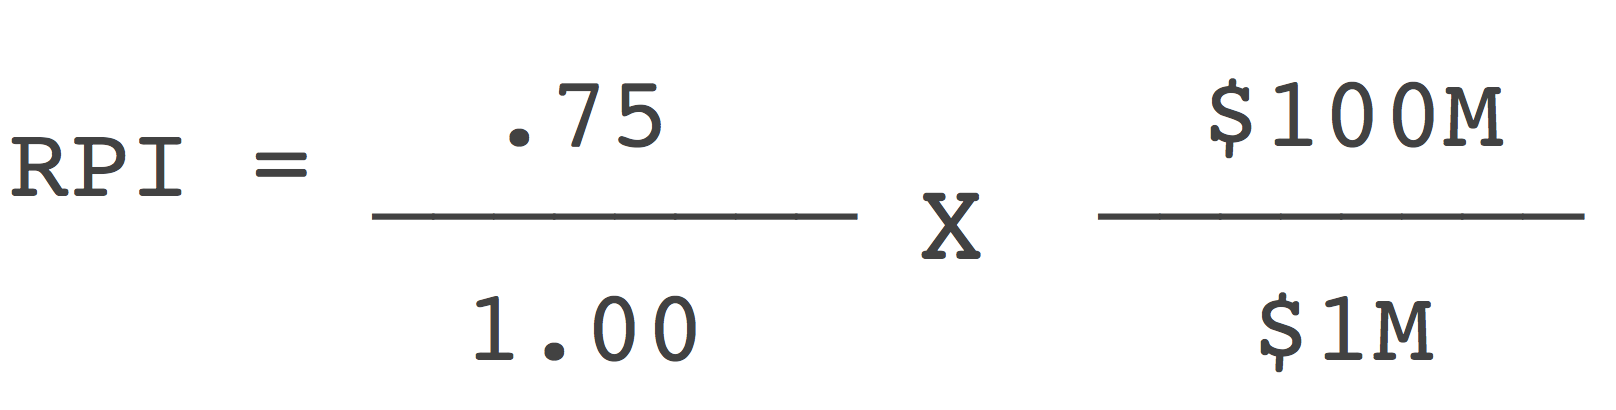
\includegraphics[width=0.8\textwidth]{test_RPI}
\end{center}

\begin{center}
\textcolor{blue}{\large RPI = .75 x 100 = 75 = 7500\% mas barato}
\end{center}

Las estimaciones, sin duda, tienen un amplio intervalo de confianza pero claramente hay una enorme eficiencia de aprendizaje para este Pretotype. Los inversores en Webvan deber\'ian haber estado dispuestos a reprimir su fiebre de la burbuja de Internet con el fin de demostrar los principales elementos de la idea antes de autorizar la soluci\'on completa.
\\ \\
Pero que se puede decir de RPI respecto al tiempo?
\\ \\
Vamos a revisar el ejemplo Voz-a-Texto de IBM para explorar la eficiencia de tiempo de Pretotyping. La f\'ormula sigue siendo la misma, pero los elementos de coste se calibran en unidades de tiempo en lugar de \$. En el c\'alculo de RPI, usted debe examinar sus expectativas: qu\'e aprendizaje y los efectos de costes que probablemente este Pretotype produzca. Aqu\'i est\'a mi cadena l\'ogica:

\begin{enumerate}

\item La soluci\'on predeterminada para IBM fue la de construir un \textit{prototipo}, no el producto completo. El prototipo podr\'ia haberles indicado, por ejemplo, el 80\% de lo que el producto final les habr\'ia indicado.

\item El \textit{pretotype} ser\'ia una prueba valiosa de apelaci\'on para el usuario b\'asico, pero quiz\'as no mostrar\'ia la luz sobre factores m\'as sutiles como por ejemplo si la forma de uso se  deteriora con el tiempo, si el uso var\'ia seg\'un la hora del d\'ia, etc. Digamos que el 50\% del producto final ser\'ia revelado.

\item Sin embargo, los par\'ametros de coste (es decir, tiempo) se muestran dram\'aticamente diferentes entre (Pro) y (Pre). En esa \'epoca, el Pro podr\'ia tomar tal vez 5 a\~nos (60 meses) para que el hardware y el software fueran lo suficientemente viables para una prueba con el cliente. El Pre por el contrario podr\'ia tomar no m\'as de 1 mes para dise\~nar.

\end{enumerate}

La l\'ogica nos entrega las siguientes variables para RPI:
\\ \\
Learning (Pre) = .50 \tab \tab \tab \tab{Learning (Pro) = .80}
\\ \\
Cost (Pro) = 60 months/meses \tab \tab {Cost (Pre) = 1 month/mes}
\\ \\
Al incluir estos n\'umeros en la f\'ormula, el tiempo RPI de este Pretotype es:

\begin{center}
    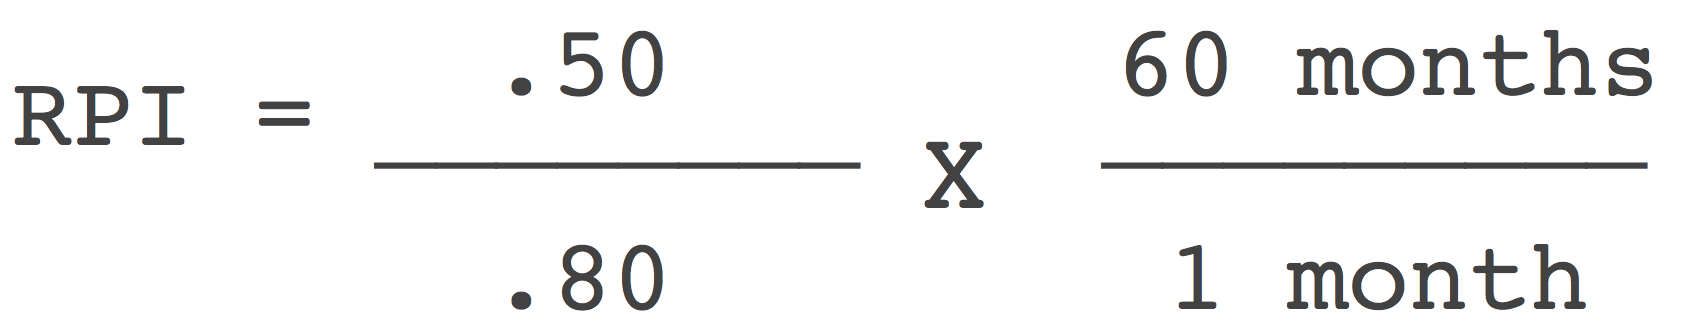
\includegraphics[width=0.8\textwidth]{tiempo_RPI}
\end{center}

\begin{center}
\textcolor{blue}{\large RPI = .62 x 60 = 37.5\% de aprendizaje mas r\'apido}
\end{center}

Por supuesto, cualquier inversor podr\'ia desafiar mi l\'ogica y ofrecer diferentes n\'umeros pero el fondo de RPI es que, bajo casi cualquier condici\'on, el costo o el aprendizaje de la eficiencia es a) masivo, y b) notablemente insensible a las estimaciones menos favorables de desempe\~no del Pre. Tome los ejemplos de Webvan o IBM y reduzca a la mitad el aprendizaje (Pre) o doble del costo (Pre): en cualquier caso, el argumento para no hacer la prueba Pretotype sigue siendo casi imposible de refutar. Todo lo que necesitas es una estimaci\'on informada del coste por el que se compite (Pro) como la l\'inea de base, adem\'as de una cadena l\'ogica de c\'omo un Pretotype adecuado se comportar\'a contra \'el (Pro).
\\ \\
NIVEL INICIAL Y CONTINUO DE INTERES (ILI / OLI)
\\ \\
El Nivel Inicial de Inter\'es (ILI), es simplemente el\% de un grupo objetivo lo suficientemente interesado en el \textbf{\textit{it}} para darle una oportunidad, o bien:

\begin{center}
    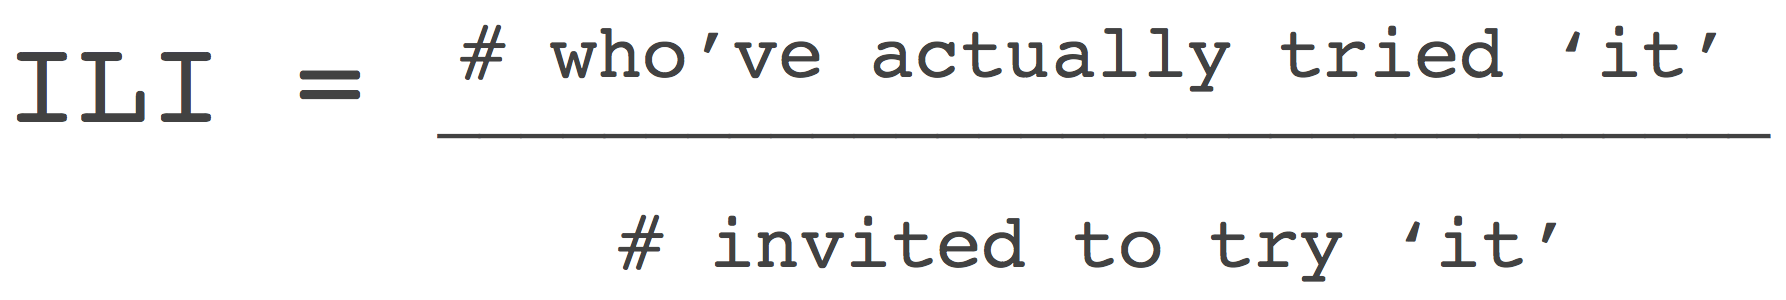
\includegraphics[width=0.8\textwidth]{ILI}
\end{center}

En otras palabras, ILI es la proporci\'on entre las personas que probaron el \textbf{\textit{it}} versus las que fueron invitadas a probar el \textbf{\textit{it}}.
\\ \\
El c\'alculo de ILI requiere la formaci\'on de un punto de vista de la cantidad de clientes a los que se desea exponer el Pretotype, que tiende a variar ampliamente dependiendo de la naturaleza del producto final y el volumen de las ventas finales que representar\'an el \'exito. Es evidente que este n\'umero objetivo de clientes ser\'a muy diferente si el que es una nueva aplicaci\'on (cientos!) frente a si se trata de una nueva l\'inea de envasado de una f\'abrica (una docena?). Igualmente, el punto de vista sobre ILI - la proporci\'on de los invitados que realmente probaron el \textbf{\textit{it}} - probablemente depender\'a de la naturaleza del producto.
\\ \\
Piense en ILI como el seguimiento de la conducta de un subconjunto de su eventual mercado objetivo:

\begin{center}
    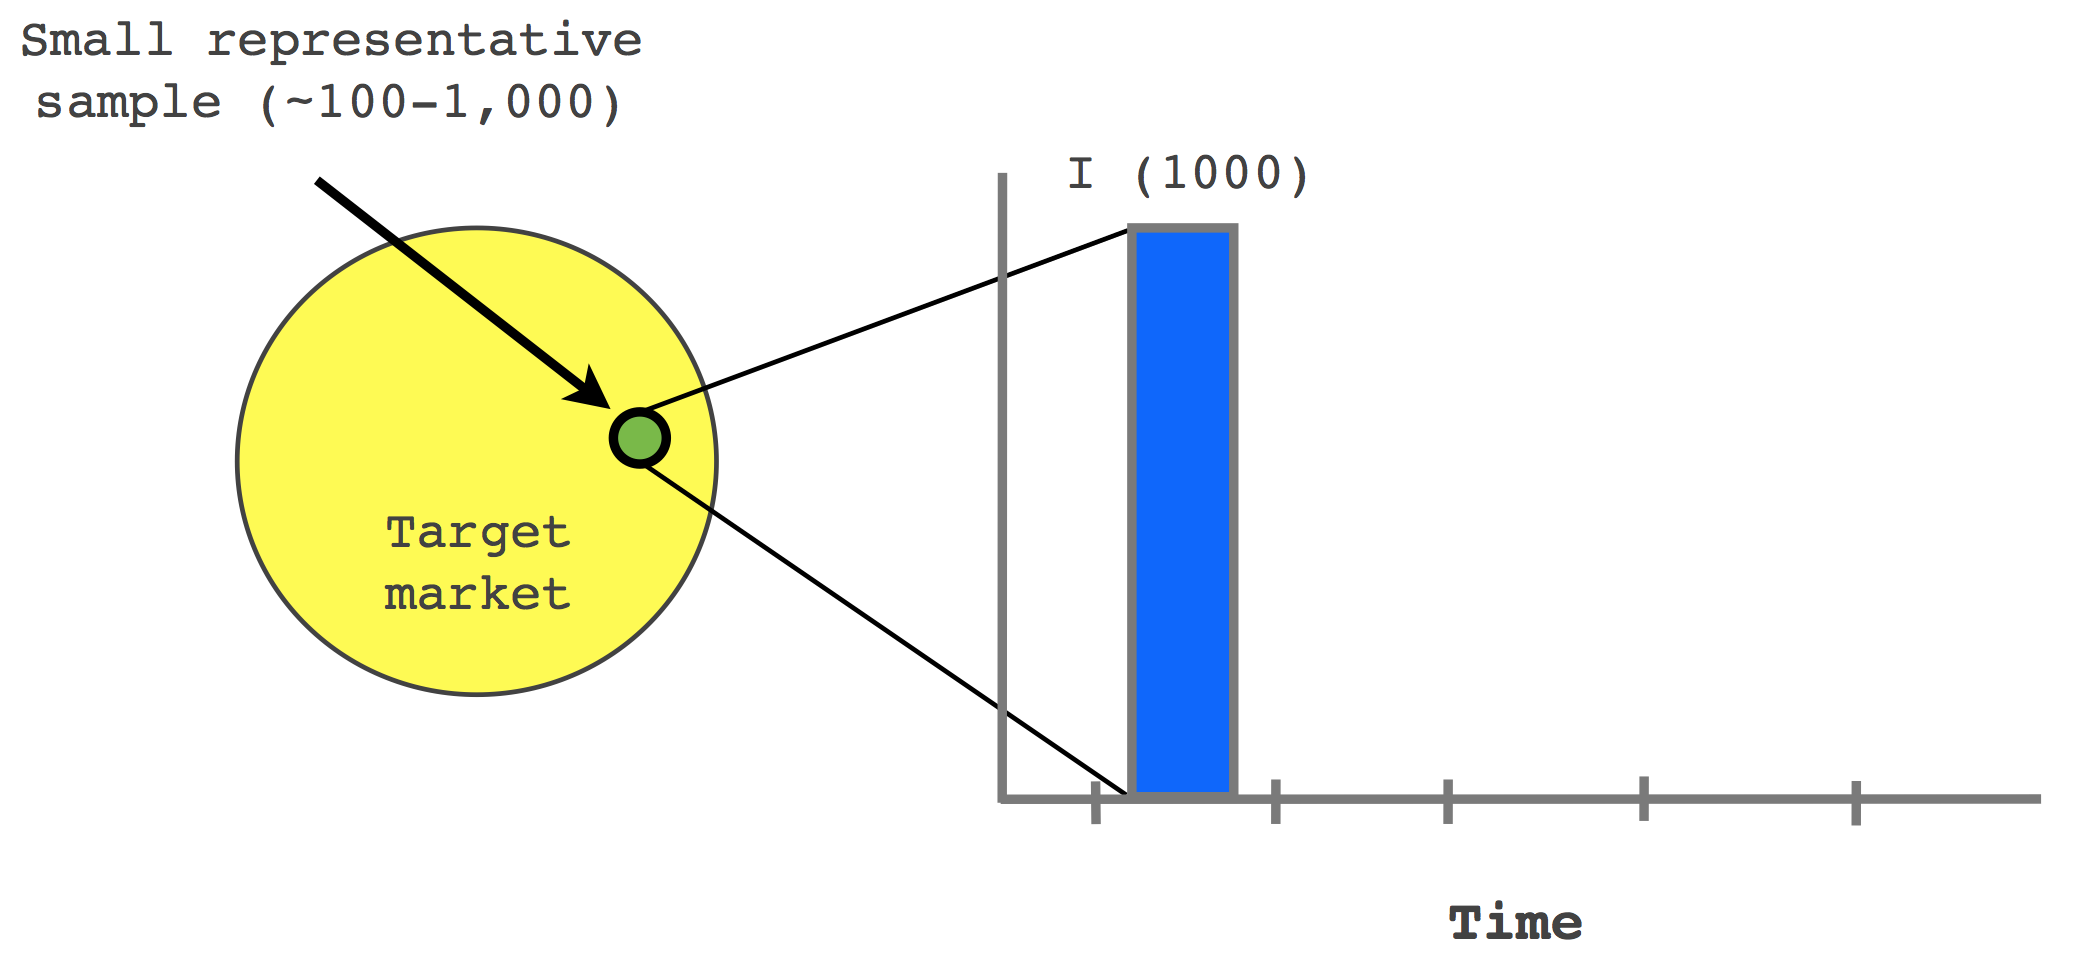
\includegraphics[width=0.9\textwidth]{ILI_graph}
\end{center}

Digamos que su grupo objetivo de clientes a los que se le expondr\'a la oferta Pretotype es 1000: llamamos a este n\'umero ``I''.  Ahora, durante el periodo en que la oferta Pretotype est\'a disponible, 741 (``T'') de esos 1000 en realidad probaron el \textbf{\textit{it}}. Su ILI es: 741/1000 o 0.741:

\begin{center}
    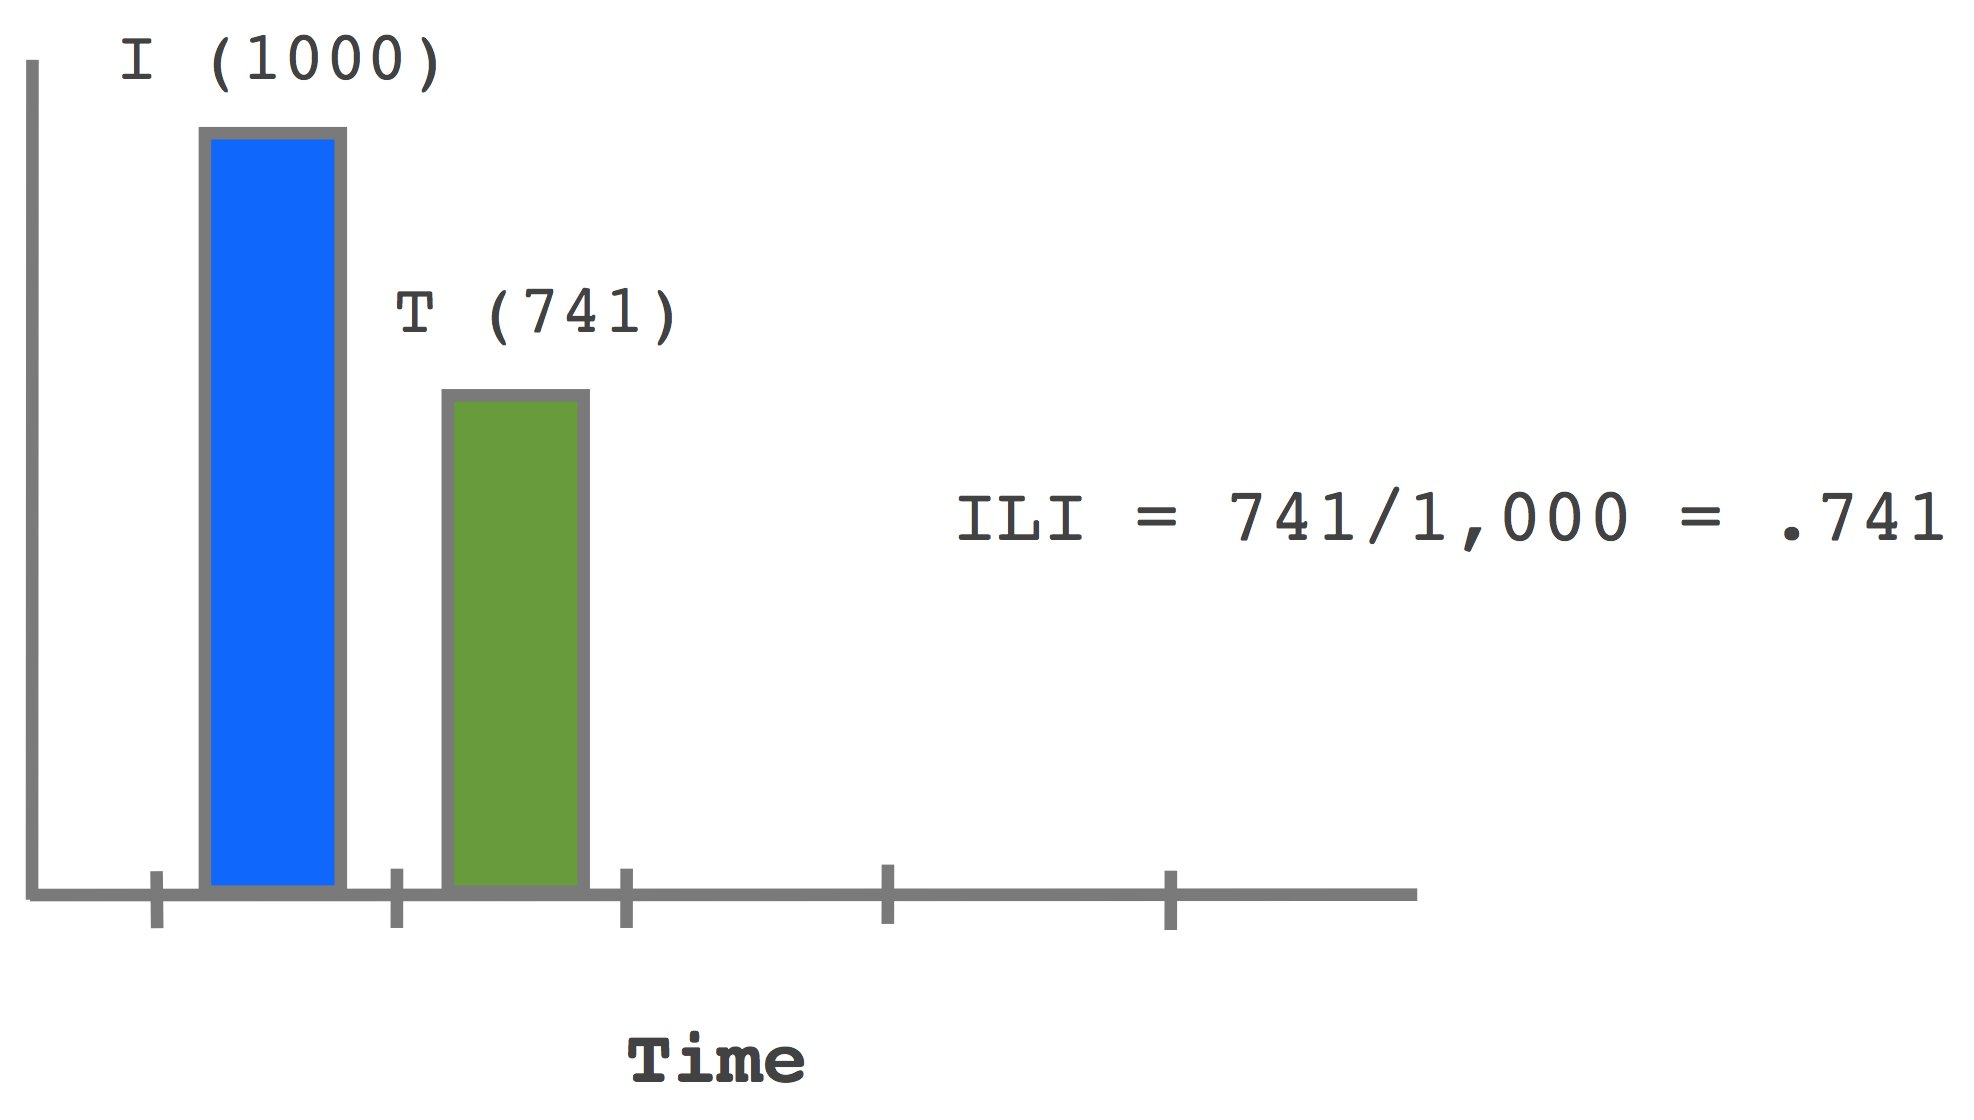
\includegraphics[width=0.9\textwidth]{ILI_example}
\end{center}

Buen comienzo! Parece que un buen \% de la muestra ha mordido el anzuelo y prob\'o de su oferta.
\\ \\
Capturar ILI es un buen comienzo pero muchas personas le dir\'an que usted puede vender cualquier cosa una vez! Para estar seguro de que tiene el \textbf{\textit{it}} apropiado, usted necesita ver cuantos clientes regresan para probar el Pretotype nuevamente.
\\ \\
En otras palabras, usted necesita medir el nivel actual de inter\'es, el \% de los que inicialmente probaron el  \textbf{\textit{it}} y que siguen usandolo/comprandolo, esto es:

\begin{center}
    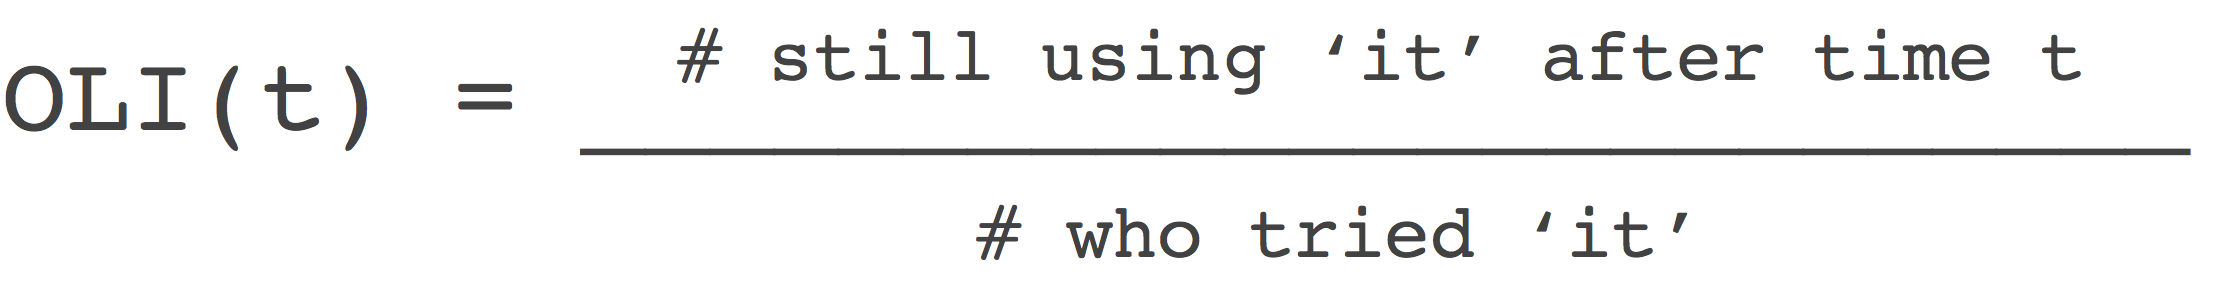
\includegraphics[width=0.8\textwidth]{OLI}
\end{center}

Tenga en cuenta que el numerador del c\'alculo ILI - la ``T'', los que est\'an probando el \textbf{\textit{it}}, se convierte en el denominador de la ecuaci\'on OLI. Si se hace un seguimiento de OLI, con el paso del tiempo normalmente muestra este patr\'on:

\begin{center}
    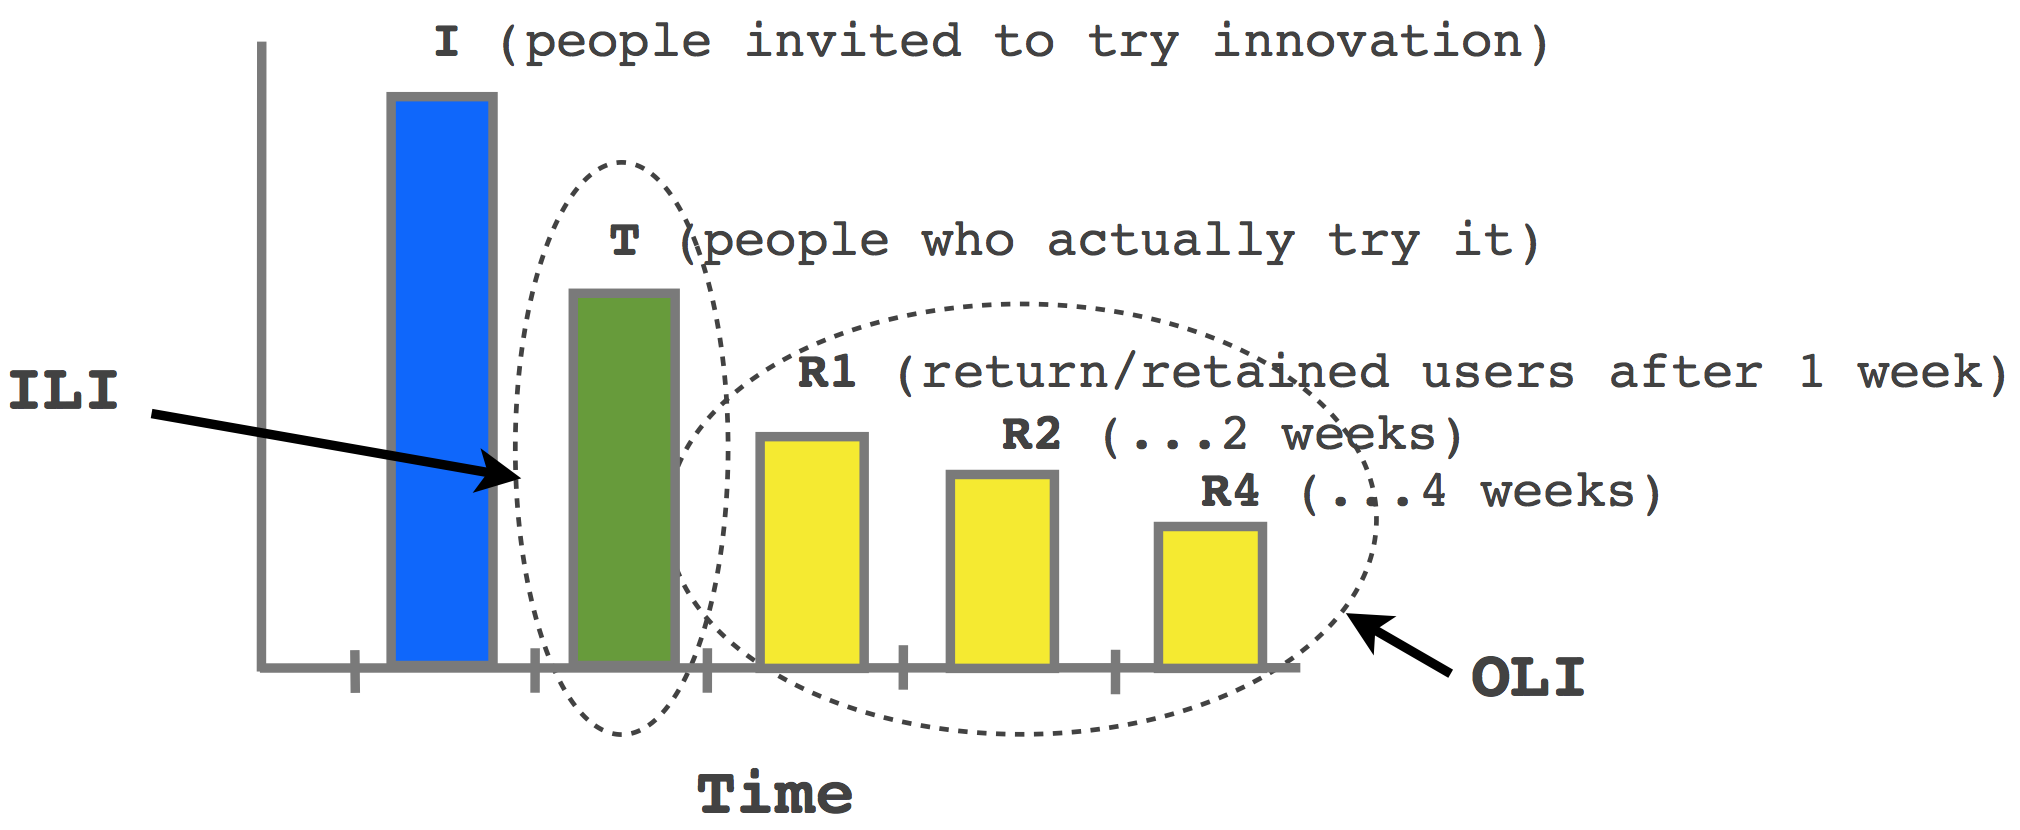
\includegraphics[width=0.9\textwidth]{OLI_2}
\end{center}

Para ilustrar esto, vamos a calcular ILI y OLI para nuestro Pretotype ficticio para Webvan. Recordemos nuestro dise\~no Pretotype MVP/Mechanical Turk: qu\'e clase de ILI alentar\'ia a\'un m\'as la inversi\'on? Al igual que con el c\'alculo RPI, la esencia de este ejercicio es construir una cadena l\'ogica que establece expectativas para validaci\'on basada en Pretotype (Pedidos de abarrotes por Internet):

\begin{enumerate}

\item Dada la ambiciosa escala de la soluci\'on completa, el Pretotype debe exponerse a una razonablemente amplia muestra representativa de las comunidades urbanas y suburbanas. Vamos a establecer un ``I'' en 10.000 personas.

\item Si bien los datos de Thoughtland sobre el \textbf{\textit{it}} de Webvan fueron abrumadoramente positivos, es muy poco probable un alto ``T'', dado que se trata de un servicio premium y no todo el mundo ver\'a la publicidad. Vamos a apuntar a un ``T'' del 5\%, osea 500.

\end{enumerate}

Lanzamos el Pretotype y digamos que nuestra respuesta inicial es 843, lo que significa que muchas personas ven la publicidad, investigan la oferta y se convierten en clientes. No es una respuesta en la escala a lo esperado por Thoughtland por ning\'un motivo, pero a\'un as\'i super\'o nuestro objetivo.

\begin{center}
    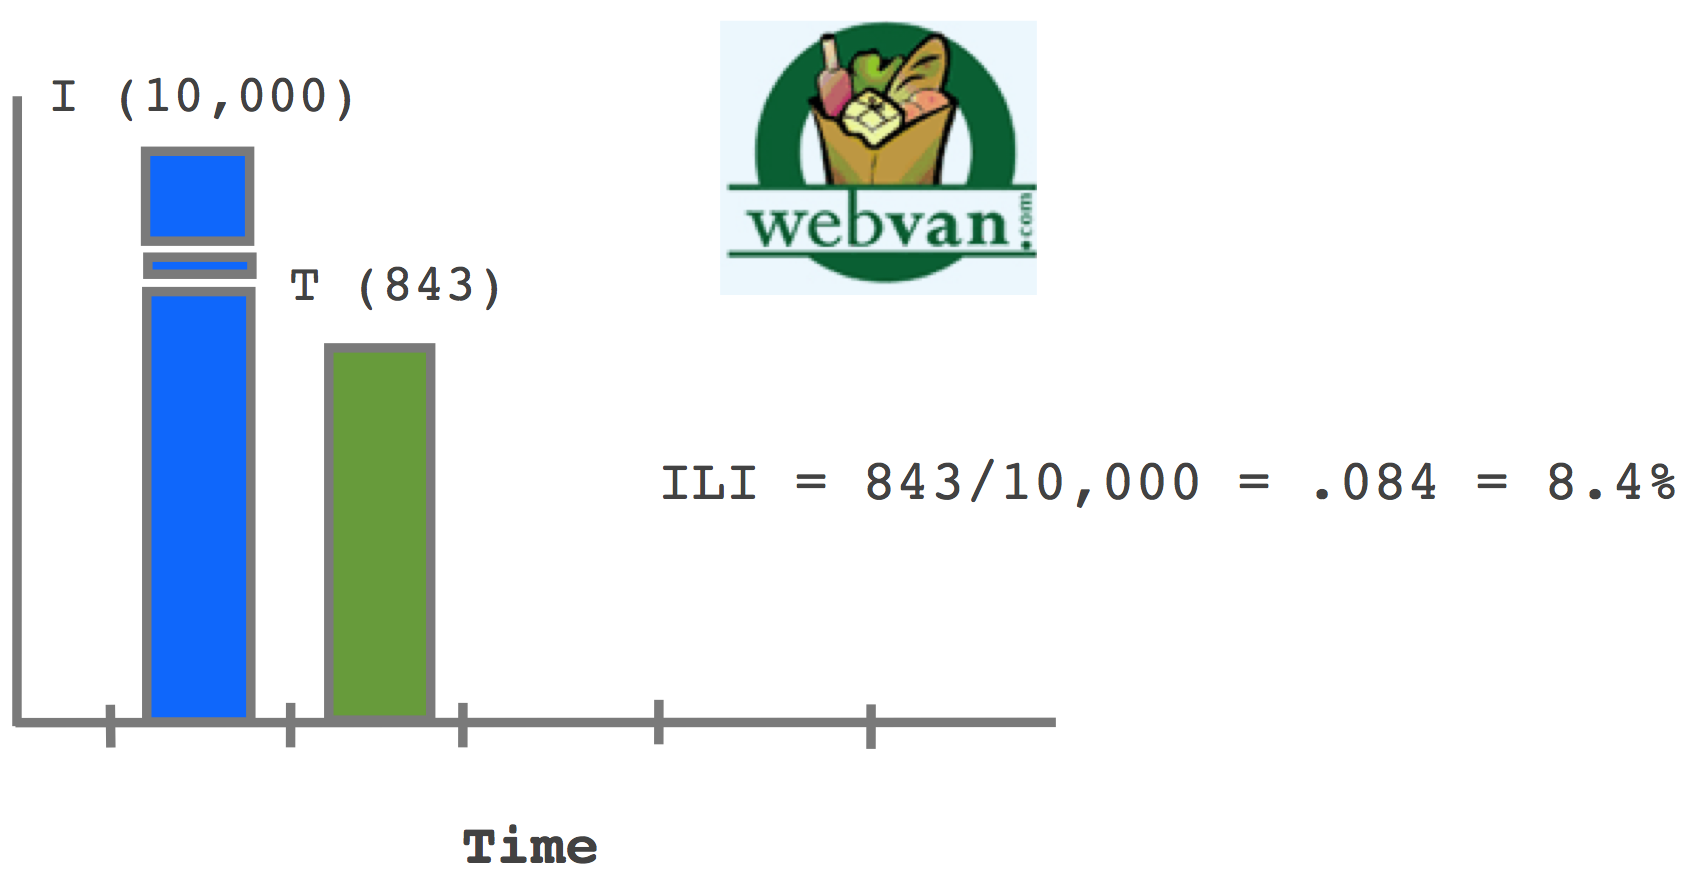
\includegraphics[width=0.9\textwidth]{ILI_weban}
\end{center}

Como inversores en Webvan, deberiamos estar animados por este resultado inicial. Pero para estar seguro que no estamos viendo el efecto ``infomercial'', decidimos continuar con el juicio por algunas semanas m\'as. Si el n\'umero de retorno de clientes, como proporci\'on de los 843 iniciales es lo suficientemente alto, vamos a saber que tenemos el \textbf{\textit{it}} correcto. Necesitamos un objetivo para OLI: vamos a aspirar a un 50\% del original 843.
\\ \\
El destino, sin embargo, no s\'olo es un amante cruel, si no que al parecer tambi\'en un comprador vol\'atil. Los datos OLI decepcionan, con cada vez menos de los 843 clientes originales regresando durante las pr\'oximas 2, 4 y 6 semanas:

\begin{center}
    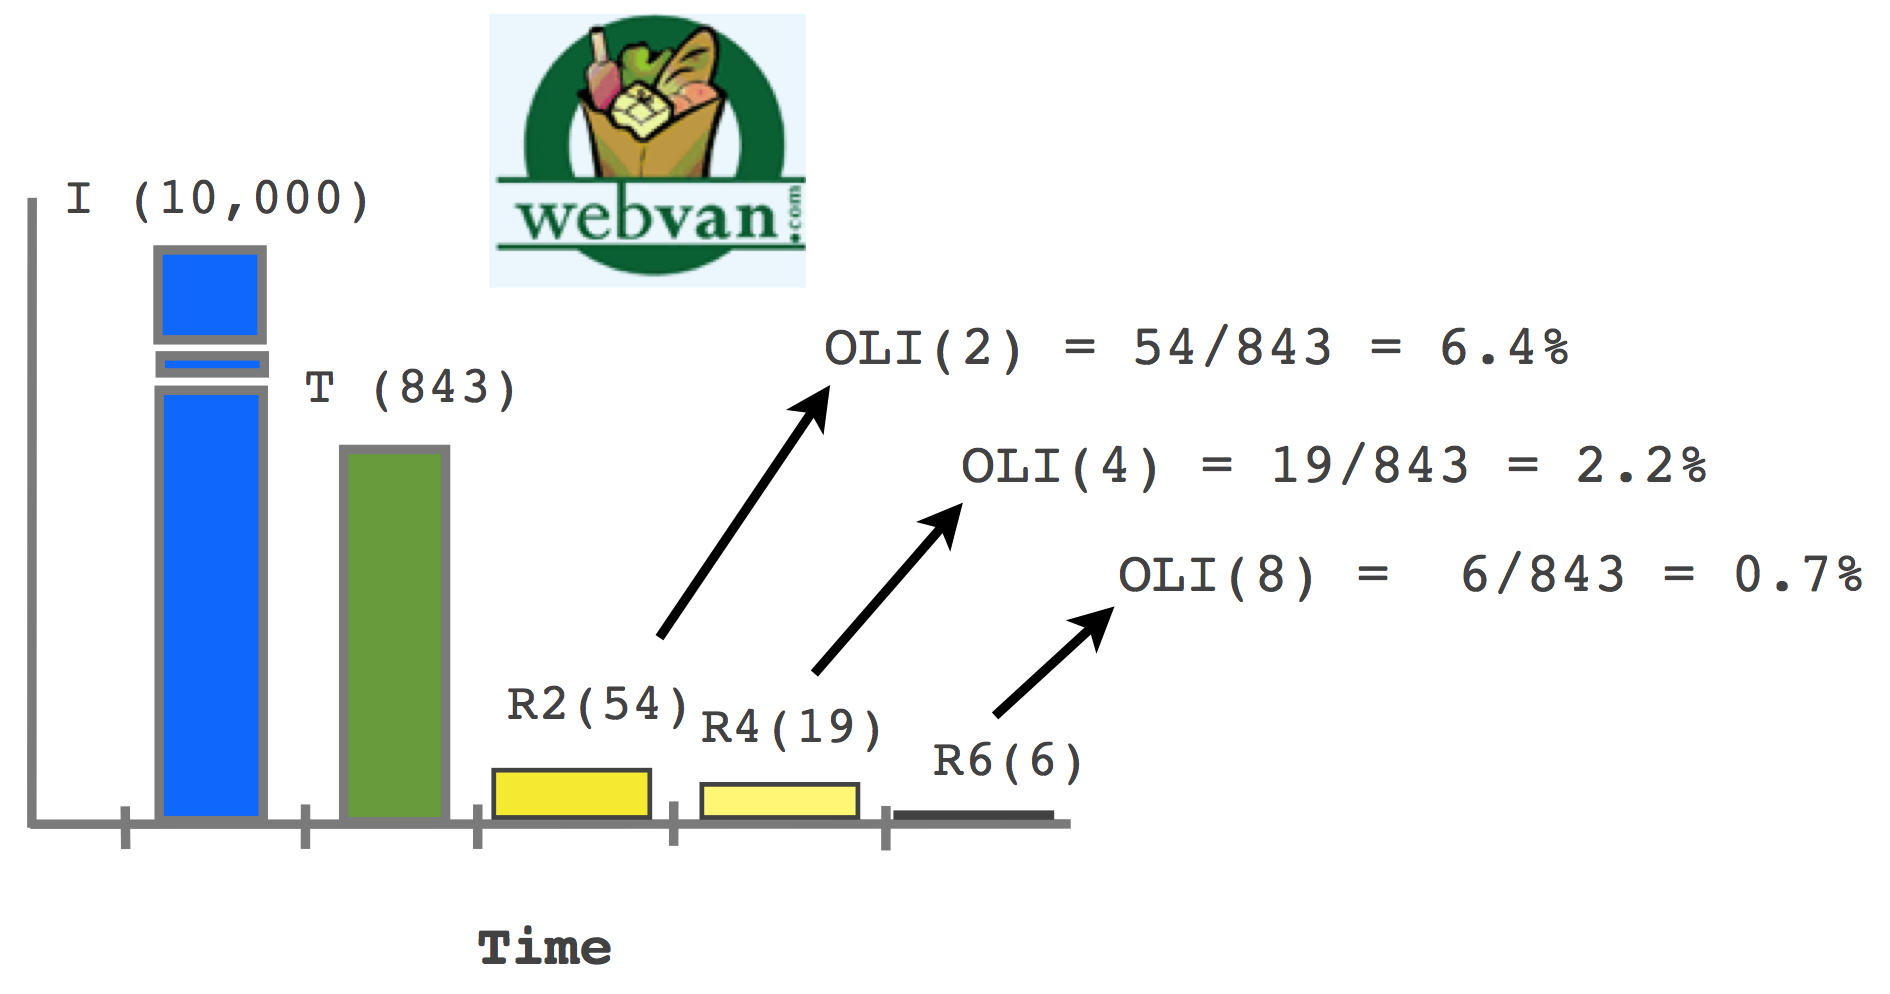
\includegraphics[width=0.9\textwidth]{OLI_weban}
\end{center}

Es evidente que la primera experiencia no alentaba a suficientes clientes para volver a los siguientes ensayos. No siempre puede ser claro el por qu\'e, pero la tendencia nos cuenta la historia. Para nuestros prop\'ositos actuales, podemos concluir que los datos muestran que despu\'es de todo, Webvan no tiene el \textbf{\textit{it}} correcto.
\\ \\
Revisando este ejemplo, la gente a menudo responde con: ``Pero el pedido de comestibles en l\'inea y entrega a domicilio es de un negocio exitoso. Mira Peapod, o Schwan's ". Esto ilustra un matiz en la definici\'on del \textbf{\textit{it}} que se est\'a probando. El \textbf{\textit{it}} de Webvan fue una prestaci\'on en todo el pa\'is prometiendo el servicio en menos de 30 minutos en 26 mercados principales, una base de clientes masiva implica una gran infraestructura: Webvan quiso ``poseer'' el comercio minorista de comestibles de alta calidad en los EE.UU.
\\ \\
Esta ambici\'on condimenta el proceso Pretotyping al estar estableciendo una meta tan alta. Nuestro Pretotype hipot\'etico, por otro lado,m gasto \$ 1 mill\'on para construir un sitio web de alta calidad, y busc\'o un alto ILI y OLI para confirmar la proposici\'on. Nuestra prueba desestim\'o el \textbf{\textit{it}}, pero eso no descarta la posibilidad de que bajo diferentes restricciones de modelo de negocio, uno parecido podr\'ia tener \'exito. Por ejemplo, Tesco, un rentable negocio de ladrillos y venta minorista de comestibles en el Reino Unido, realiz\'o un Pretotype para pedidos en l\'inea mediante el uso de sus tiendas, empleados y veh\'iculos. Ahora Tesco.com se considera como otro canal para llegar a los clientes existentes. En otro caso, Peapod fue otro pure-play que controlaba su expansi\'on proporcionando un servicio s\'olo cuando su principales partes interesadas (Dutch international grocery outlet operator Royal Ahold) tenian instalaciones de distribuci\'on existentes.
\\ \\
Los inversores pueden considerar Pretotyping como un m\'etodo para modelar una estrategia de bajo costo, tocando diferentes escenarios hasta que la mezcla correcta de caracter\'isticas del producto, instalaciones de ejecuci\'on, la comercializaci\'on, los precios y las asociaciones se puedan probar. En el ejemplo Webvan, los inversores pudieron optar por bajar su tienda de campa\~na despu\'es de la primera ronda, o repensar el modelo de negocio e intentar otra prueba Pretotype.
\clearpage

\subsection{Creando Confianza Incrementalmente}

Pretotyping, y las m\'etricas de RPI, ILI y OLI que lo apoyan, son una ilustraci\'on pr\'actica del Teorema de Bayes. Thomas Bayes fue un matem\'atico Ingl\'es del siglo 18 y ministro Presbiteriano. Su teorema explica c\'omo una creencia subjetiva deber\'ia cambiar de forma racional para dar cuenta de (nueva) evidencia:

\begin{center}
\textbf{CREENCIA INICIAL + NUEVA DATA = CREENCIA MEJORADA}
\end{center}

Pretotyping es una b\'usqueda r\'apida, pero estructurada de nueva evidencia sobre la cual podemos basar un cambio en nuestra expectativa de las posibilidades de \'exito.
\\ \\
Bayes proporciona la f\'ormula matem\'atica mediante la cual las probabilidades se pueden ajustar para nueva evidencia, y aunque la ecuaci\'on es lo suficientemente potente como para considerar los aspectos cr\'iticos de la vida moderna (por ejemplo, la detecci\'on de spam de Gmail), no tenemos que bucear en la mec\'anica aqu\'i. El aprendizaje clave es que los inversores deber\'ian tratar de aumentar la confianza de forma \textit{incremental}, y en base a la \textit{evidencia}.
\\ \\
Esto implica muchas reuniones cortas para analizar datos con los inventores, el objetivo es o bien bajar las espectativas o aumentar la \textit{creencia} en el \'exito del proyecto. En la mayor\'ia de los casos, el resultado de una prueba Pretotype ser\'a clara, y gracias a la primera Ley del Fracaso, enf\'atizo: Usted tiene el \textbf{\textit{it equivocado}}! En unos pocos casos, los datos entregaran una confirmaci\'on alentadora: usted tiene el \textbf{\textit{it correcto}}!
\\ \\
Pero, Los inversores, c\'omo deben interpretar los resultados de las pruebas Pretotype ambiguas? Esto puede, por supuesto, ser una cuesti\'on de prueba-simpleza: si una prueba intenta responder demasiadas preguntas a la vez, puede ser dif\'icil atribuir un significado claro para los resultados. M\'as all\'a de esta cuesti\'on, c\'omo se manejan los resultados de pruebas que no alcancen los objetivos ILI y OLI, pero que superan el nivel de fracaso?
\\ \\
RPI es la respuesta: la conclusi\'on de los experimentos Pretotype es tan robusta que se debe ejecutar uno o m\'as Pretotypes adicionales hasta que se obtenga una clara tendencia en los resultados. Todo esto para recuperar y ampliar nuestro di\'alogo idealizado entre inventores e inversores:

\begin{enumerate}

\item AMBOS: Comentan y convergen en algunas preguntas tipo ``Lo quieren?''

\item INVENTOR: Dise\~nar el Pretotype m\'as simple que pueda para responder esas preguntas.

\item AMBOS: Acordar umbral superior (``it correcto'') y el umbral inferior (``it incorrecto'') para las expectativas para ILI, esto antes de la prueba.

\item INVENTOR: Se ejecuta el test, se confirma el ILI obtenido.

\item AMBOS: Acordar si ILI sugiere continuar. Si es as\'i, acordar un objetivo razonable para OLI y el ritmo de repetici\'on adecuada (R = 7 d\'ias, R = 14 d\'ias, etc) y reunirse de nuevo despu\'es de cada hito R para revisar el progreso. La decisi\'on se basar\'a en la tendencia OLI que se visualiza:

\end{enumerate}

\begin{center}
    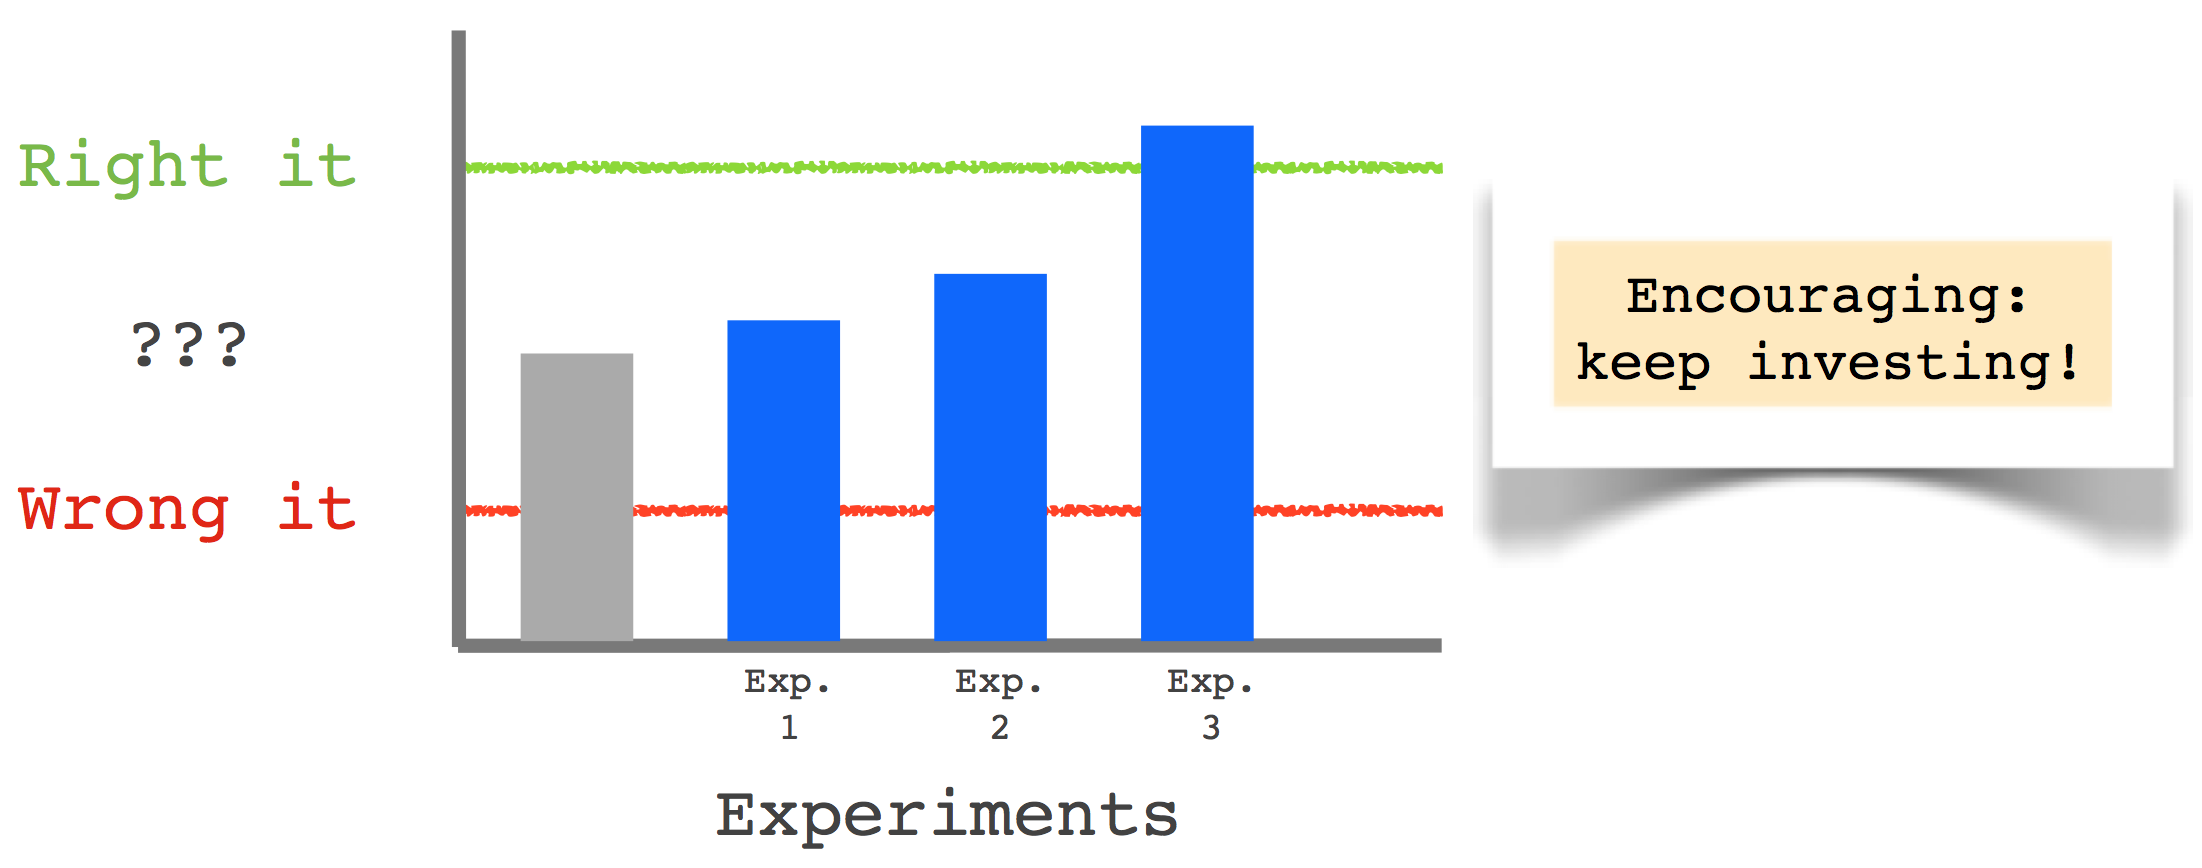
\includegraphics[width=0.9\textwidth]{experimento_1}
\end{center}

\begin{center}
    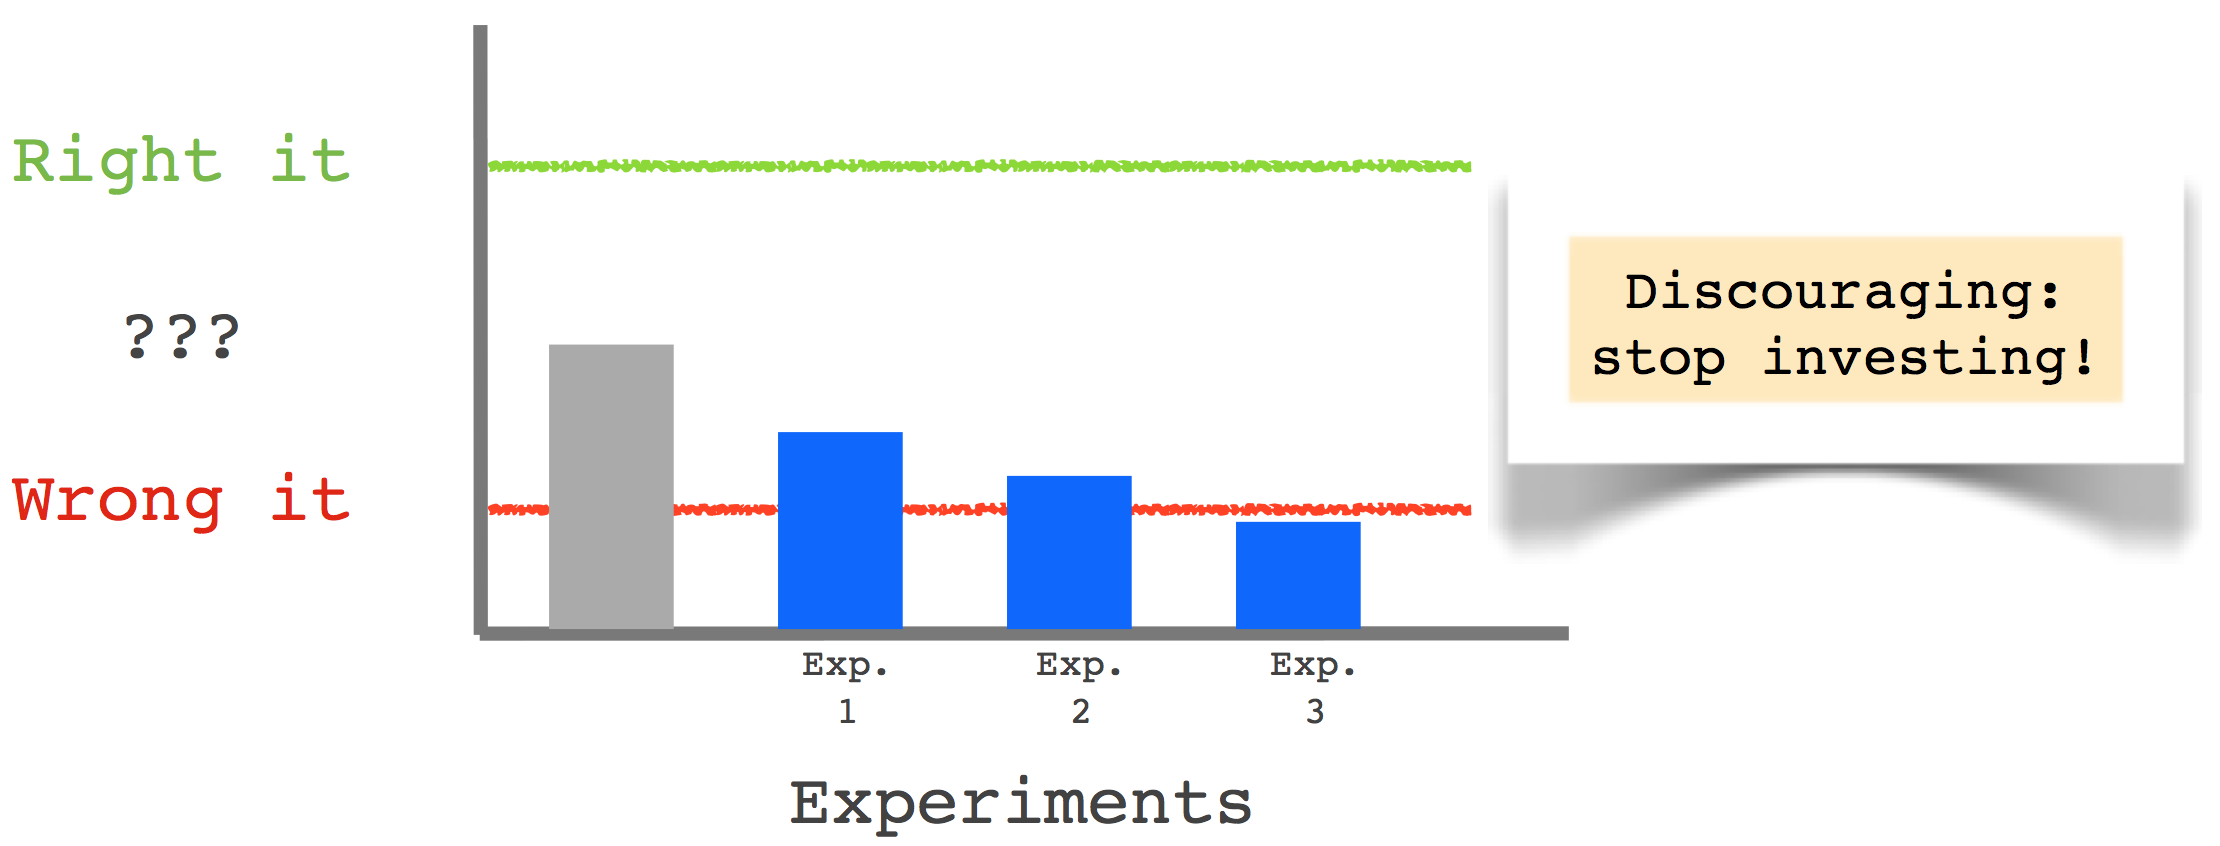
\includegraphics[width=0.9\textwidth]{experimento_2}
\end{center}

\begin{center}
    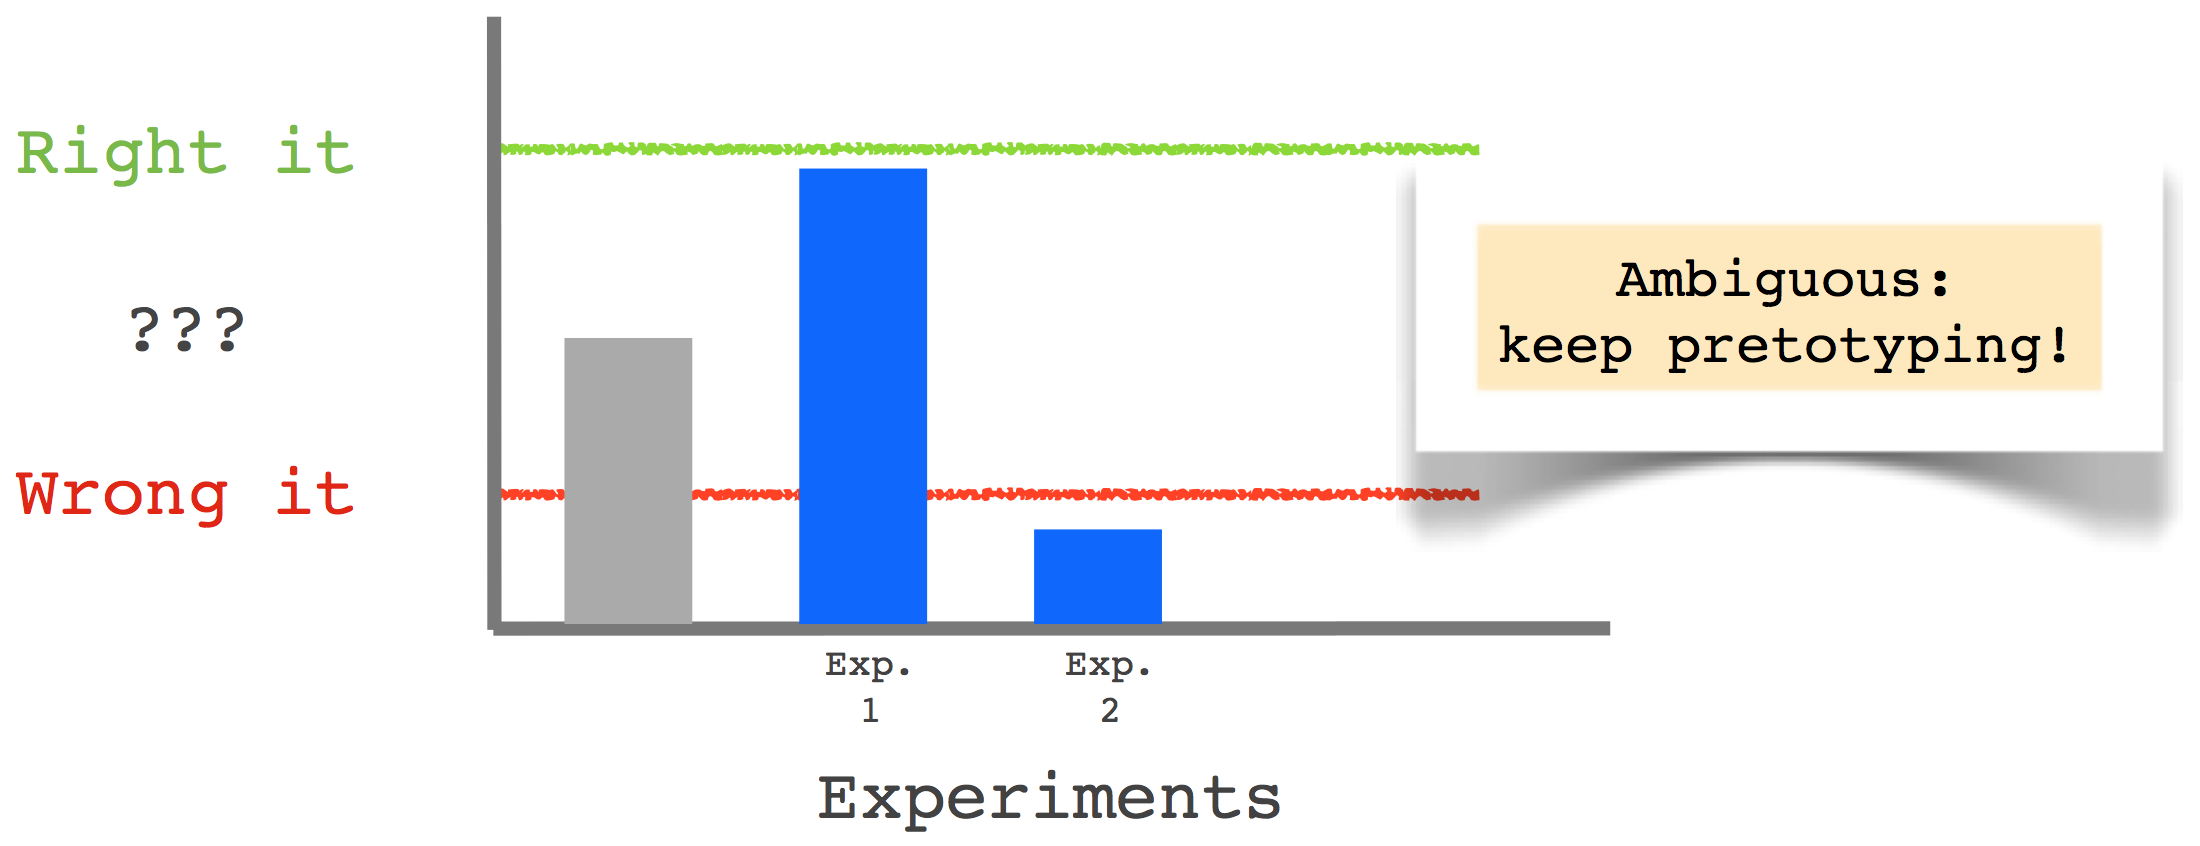
\includegraphics[width=0.9\textwidth]{experimento_3}
\end{center}

La discusi\'on de este tema no estar\'ia completa sin introducir el \textit{dead cat bounce}. Este encantador t\'ermino es utilizado por los inversionistas de Wall Street para denotar un repunte alentador en un mercado que esta yendo a la baja. La referencia es al hecho de que incluso un gato muerto rebotar\'a una vez si se cae o es pateado lo suficientemente fuerte. De hecho, los cient\'ificos han sabido por mucho tiempo que casi cualquier sistema natural puede ser estimulado para producir una respuesta involuntaria (pensar en la prueba de reflejo con un martillo). Un ejemplo cl\'asico de la historia de los negocios es el Efecto Hawthorne, en el que la productividad de una f\'abrica aumenta en respuesta a los cambios tanto positivos como negativos de los niveles de iluminaci\'on administrados por los investigadores.
\\ \\
La relevancia de Pretotyping es que los inversores en una etapa temprana pueden influir en el resultado de los experimentos que financian, por lo que deben estar atentos al riesgo de crear las condiciones para un \textit{dead cat bounce}. Los inversores deben establecer una meta alcanzable para el ``\textbf{\textit{it}} correcto'', proporcionar suficientes recursos - por lo general tiempo - para el equipo Inventor para construir y ejecutar la prueba Pretotype, a continuaci\'on, examinar los datos ILI cuidadosamente antes de tomar la decisi\'on sobre continuar o no. Los inventores siempre querr\'an probar m\'as pruebas, hay que estar firmes e insistir en que "los n\'umeros son los que hablan".
\clearpage

\subsection{Pretotyping para todo}

Hasta ahora hemos discutido una gama de productos y servicios orientados al consumidor y en nuestros casos de estudio proponemos invitar a una muestra bastante amplia de potenciales clientes para probar el Pretotype. Para muchos inversionistas, sin embargo, el panorama es muy diferente a este cl\'asico ("B2C") Modelo Business-to-Consumer, pero yo dir\'ia que el m\'etodo Pretotyping puede adaptarse para apoyar la innovaci\'on dentro de estos contextos tambi\'en.
\\ \\
INNOVACION INTERNA O PROCESOS
\\ \\
Los estudios\footnote{En el Journal of Economic Behavior, Vol. 50 (2003), Stephanie Rosenkranz sugiere que el 60\% del esfuerzo de innovaci\'on fue a la innovaci\'on interna.} indican que para muchas empresas, la mayor parte de sus recursos de innovaci\'on van hacia la innovaci\'on interna, es decir, cambios en los procesos, la introducci\'on de sistemas, iniciativas de calidad. Todas estas innovaciones tienen el potencial de reducir costos o mejorar la experiencia del cliente final, lo que contribuye indirectamente a la preservaci\'on o el aumento de los ingresos y beneficios.
\\ \\
Pretotyping es un m\'etodo muy adecuado para probar la eficacia ``\'exito'') de una innovaci\'on interna (``\textbf{\textit{it}}'') con un determinado grupo de empleados ``clientes''. Con un nuevo producto o servicio, la incertidumbre relacionada bajo estudio es "lo quieren?"; con innovaciones internas, la incertidumbre es una variante de ``Van a cumplir?'' (por ejemplo, usar el nuevo proceso, cambiar al nuevo sistema, aplicar la capacitaci\'on para el nuevo trabajo, etc.) As\'i que la clave para aplicar Pretotyping a las innovaciones internas es aislar la pregunta ``Van a cumplir?'' antes de elegir el m\'etodo Pretotype correcto y ejecutar la prueba.
\\ \\
BUSINESS-TO-BUSINESS (``B2B'')
\\ \\
Las empresas que operan en un ambiente (``B2B'') Business-to-Business, t\'ipicamente venden componentes o subcomponentes a otras empresas que a continuaci\'on, los convierten en productos terminados. Los clientes en este contexto, por lo general son menores en n\'umero pero individualmente mucho m\'as importantes para el \'exito de la empresa. Esto aumenta las expectativas para aplicar pretotyping a nuevos productos y servicios: pocas empresas B2B estar\'an dispuestas a poner en peligro las relaciones con clientes valiosos con una oferta fake door especulativa.
\\ \\
La soluci\'on en este caso es la transparencia y el enfoque. Las empresas B2B deben comenzar por la negociaci\'on de la pr\'actica empresarial de pretotyping con uno o m\'as clientes (preferiblemente el  m\'as progresista). Esto elimina las preferencias ``ciegas'' en comparaci\'on con pretotypes B2C, pero el valor de conservar la  relaci\'on a trav\'es de la transparencia vale la pena el sacrificio. El acuerdo deber\'ia definir los l\'imites de la actividad pretotyping; por ejemplo cu\'antos experimentos se llevar\'an a cabo por a\~no y circunscribir las categor\'ias de productos y procesos de negocio que pueden estar dentro del alcance.
\\ \\
La segunda adaptaci\'on es limitar los modos pretotype a los cuatro m\'as amigables con el cliente: Pinocchio, Mechanical Turk, One Night Stand y el MVP.
Fake door e impersonator son menos pr\'acticos en un contexto B2B.
\\ \\
Otra diferencia clave en el entorno B2B es que muchas innovaciones imponen cambios en el proceso por parte del cliente, y los ``costes de adaptaci\'on'' de esos cambios pueden sesgar la receptividad del cliente respecto a la innovaci\'on. Por esta raz\'on, aplicar pretotyping a nuevos procesos puede evitar a menudo confrontaci\'on entre el proveedor y el cliente, cuando la empresa proveedora intenta forzar la innovaci\'on en el cliente.
\\ \\
NEGOCIOS CON EL GOBIIERNO (``G2B'') O EL CONTRIBUYENTE (``G2T'')
\\ \\
Organismos del sector p\'ublico p tambi\'en pueden utilizar Pretotype para servicios, desde nuevas pol\'iticas fiscales a la prestaci\'on de servicios financiados por los contribuyentes, como la recolecci\'on de basura. Al igual que en el contexto B2B, un grado de transparencia es recomendable. Los ciudadanos han sido en general entusiastas sobre el uso de las redes sociales, plataformas de crowdsourcing y la idea de hacer participar a votantes y contribuyentes en la labor de formulaci\'on de pol\'iticas. Pretotyping nuevas pol\'iticas, leyes o servicios ser\'ia el siguiente paso en la democracia interactiva.
\\ \\

\centerline{--------------------------------------------------------}

ARGUMENTOS FINALES
\\ \\
Las Leyes del fracaso existen para cualquier innovaci\'on, el \'exito es extremadamente raro. Pretotyping aporta pruebas r\'apidas y disciplinadas para testear innovaciones de \'ultima generaci\'on, lo que permite Inventores e inversores:

\begin{itemize}

\item \textbf{Inventar como una Startup:} Las empresas deben experimentar muchas ideas, tanto lass obvias (posibles falsos positivos, como Webvan) y las que suenan a locura (posibles falsos negativos, como Twitter).

\item \textbf{Invierta como un adulto:} Las empresas deben invertir en innovaciones de vanguardia basadas en la evidencia y los datos, no en opiniones o especulaciones. La evidencia se acumula gradualmente y genera confianza, entonces la inversi\'on debe fluir.

\end{itemize}

Pretotyping cambia como Inventores e Inversores hablan entre s\'i, de tal manera que su inter\'es mutuo consiste en reunir datos de manera eficiente, sin dar espacio a especulaciones. Pretotyping no se traduce en un menor n\'umero de fracasos, pero los fracasos llegar\'an mas r\'apido. Esto conserva los recursos de innovaci\'on a fin de que el peque\~no n\'umero de \textbf{\textit{``it correctos''}} pueda ser identificado y acogido r\'apidamente.
\\ \\
Use pretotyping en su negocio si usted quiere fallar (r\'apido)!
\clearpage

\section{ANEXO 1 - HOJAS DE TRABAJO PRETOTYPING}

Hojas de trabajo para dise\~no de experimento PretoStorming
\\ \\
Metricas Pretotyping I - Calculando RPI e ILI
\\ \\
Metricas Pretotyping II - Calculando OLI
\clearpage
 
\begin{center}
    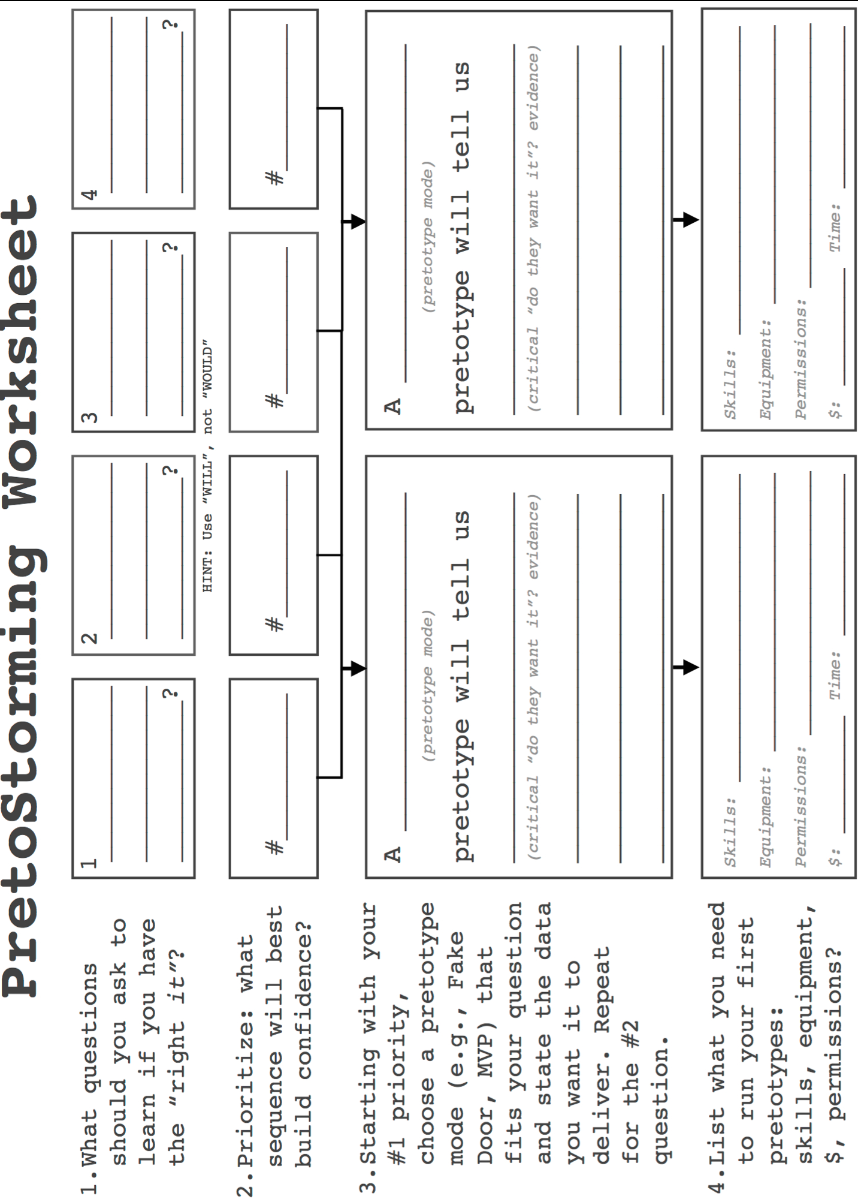
\includegraphics[width=1.1\textwidth]{pretostorming.png}
\end{center}
\clearpage

\begin{center}
    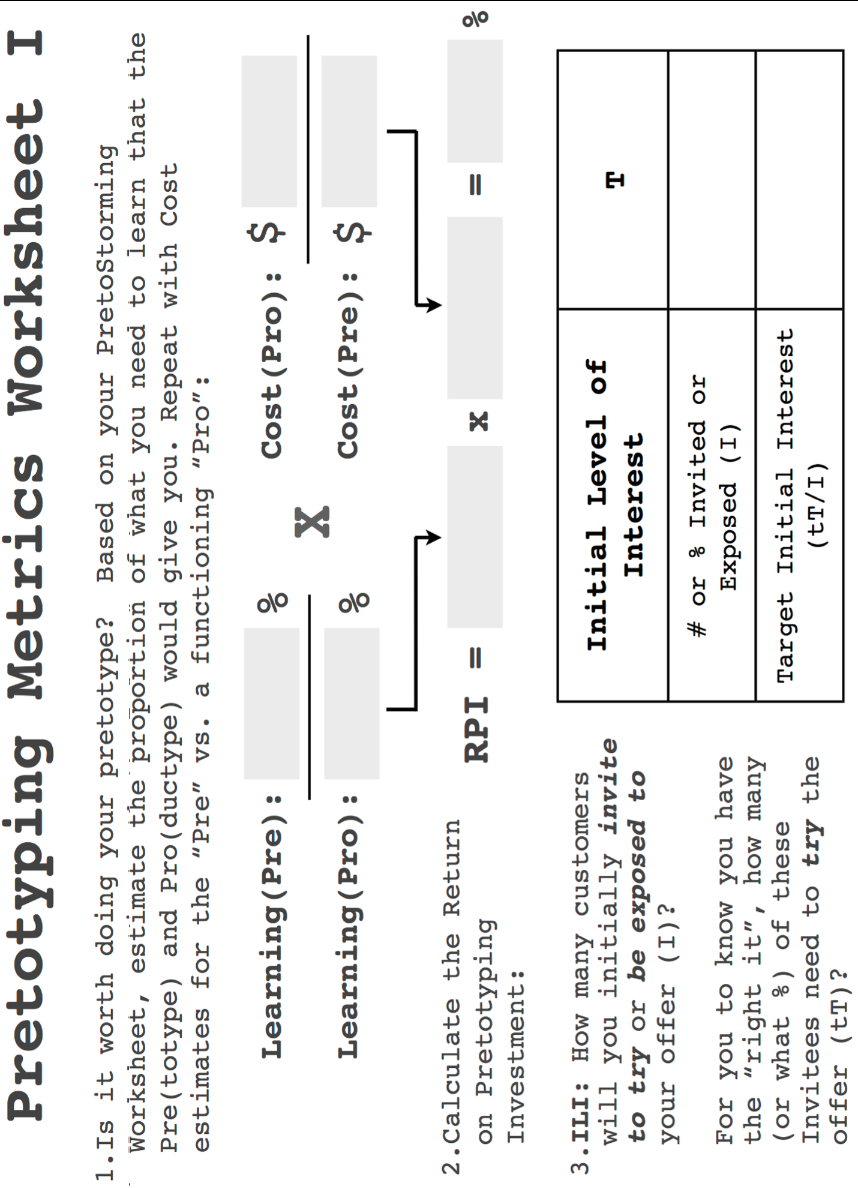
\includegraphics[width=1.1\textwidth]{metrics_1.png}
\end{center}
\clearpage

\begin{center}
    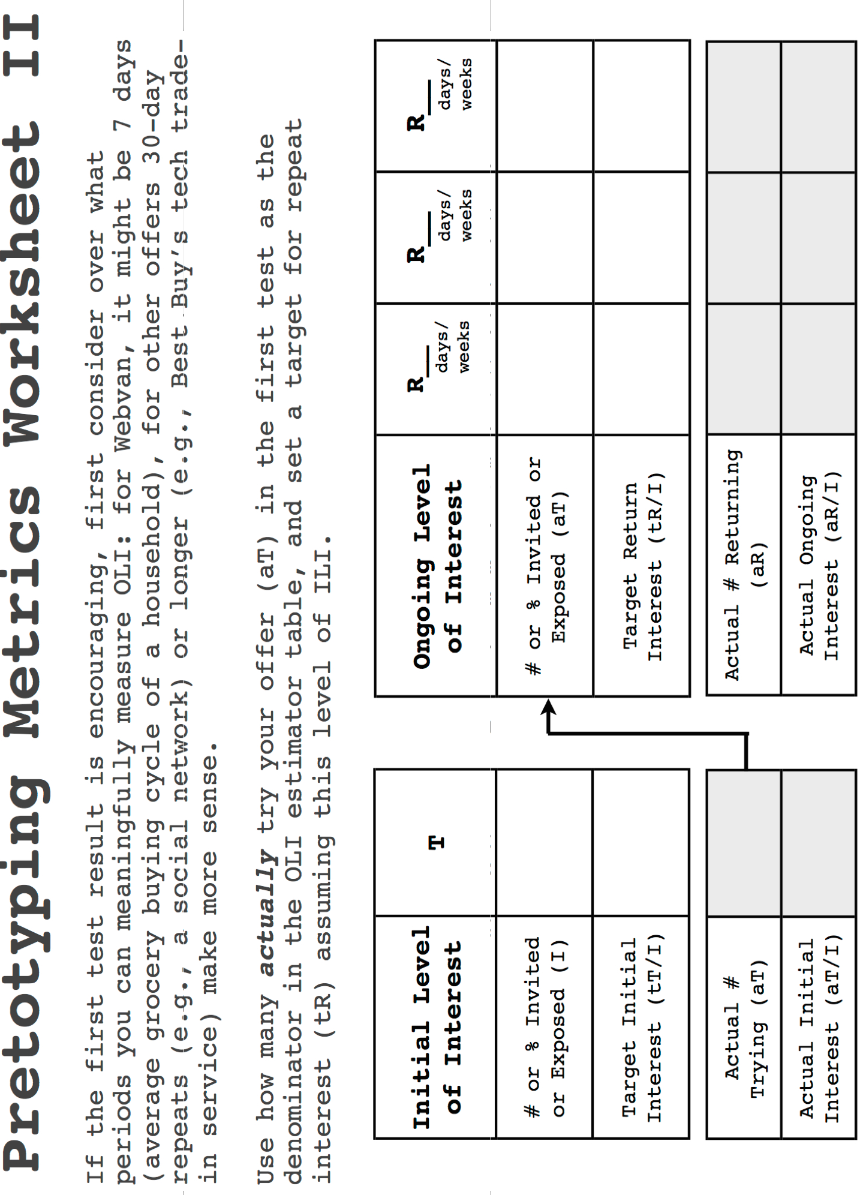
\includegraphics[width=1.1\textwidth]{metrics_2.png}
\end{center}
\clearpage

\section{ANEXO 2 - ACERCA DEL AUTOR}

Jeremy Clark es un estratega en constante crecimiento y experto en innovaci\'on, ayudando a las empresas a dar rienda suelta a la innovaci\'on durante m\'as de 20 a\~nos. Como consultor, ha entrenado a l\'ideres empresariales de multiples sectores a trav\'es de proyectos de innovaci\'on y estrategia de crecimiento, tambi\'en ha ayudado a crear cientos de millones de d\'olares con productos y servicios innovadores. Muchos de \'estos son marcas altamente visibles, otros se desarrollan como innovaciones a procesos internos o B2B, los que presentaron soluciones para los clientes OEM.
\\ \\
Antes de convertirse en un consultor independiente, Jeremy fue director de Strategos, la empresa fundada por el experto en gesti\'on, el profesor Gary Hamel, Jeremy sigue prestando apoyo al \'ultimo proyecto de Hamel, Management Innovation eXchange (o MIX). Jeremy co-fund\'o los Laboratorios Pretotype con Alberto Savoia el 2012 para introducir t\'ecnicas de innovaci\'on agiles para complementar los enfoques m\'as tradicionales para madurar la innovaci\'on en las empresas, tales como laboratorios de I + D y los procesos de DNP estructurados.
\\ \\
Jeremy recibi\'o su MBA en la Universidad de Chicago y es un orador frecuente en la estrategia y la innovaci\'on.
\\ \\
Jeremy es un experto en empresas de riesgo, un enfoque que integra principios de emprendimiento y m\'etodos dentro de las empresas. Cada vez esta mas involucrado en ayudar a las empresas a aprovechar el poder de los medios sociales para involucrar a las comunidades y grupos de clientes en el trabajo de innovaci\'on de las empresas.
\\ \\ \\
Contacto:  jeremy@fxxinc.com o visitar www.pretotypelabs.com
\clearpage

\section{ANEXO 3 - ACERCA DE LA TRADUCCION}

Esta traducci\'on a sido posible gracias al invaluable aporte que Pretotype puede entregar a las organizaciones. Oscar Rubio y Rodrigo Valdes conocieron Pretotype mientras investigaban herramientas para facilitar la innovaci\'on. Fue tanto el potencial que vieron en Pretotype, que se comunicaron con Jeremy para ofrecer la traducci\'on de Pretotyping@Work al idioma Espa\~nol.
\\ \\
Ambos suman mas de 10 a\~nos de experiencia en el \'ambito profesional relacionado con la innovaci\'on y las tecnolog\'ias de la Informaci\'on. Esta experiencia les ha dado una visi\'on global de la industria, esto les ha permitido identificar patrones comunes entre distintas organizaciones en donde hay espacio para la mejora. La propuesta es generar mayor valor e innovaci\'on mediante herramientas y paradigmas modernos de tecnolog\'ias de la Informaci\'on.
\\ \\
Actualmente Oscar y Rodrigo se encuentran levantando \textit{CyberSyn}, su propia empresa para prestar servicios de mejora e innovaci\'on (\textit{DevOps}) a organizaciones de habla hispana.
\\ \\
Ambos recibieron sus t\'itulos de Ingenieros en las ciencias de la Inform\'atica en la Universidad del Bio-Bio y en la Universidad Cat\'olida de la Sant\'isima Concepci\'on, Regi\'on del Bio-Bio, Chile.
\\ \\ \\
Contactos:
oscar.rubio.ma@gmail.com o visitar www.cybersynforce.com
\\ \\
rodrigovaldes@gmail.com o visitar www.cybersynforce.com


\end{document}